\documentclass[xcolor=table,ps]{beamer}
\usepackage{listings}
\usepackage[spanish]{babel}         
\usepackage[utf8x]{inputenc}      
\usepackage{multirow}
\usepackage{colortbl}
\usepackage{ltablex}
\usepackage{courier}
\usepackage{subfigure}
\usepackage{wrapfig}
\usepackage{ragged2e}
\usepackage{setspace}
\usepackage{caption}
\usepackage{adjustbox}
\usepackage[justification=centering, labelformat=empty]{caption}
\captionsetup[figure]{font={stretch=0.5}}
\usepackage{cancel}
% \usepackage{subfig}
%%%%%%%%%%%%%%%%%%%%%%%%%%%%%%%%%%%%%%%%%%%%%%%

%\usetheme{Boadilla}
\usetheme{Madrid}
\setbeamertemplate{navigation symbols}{}
\setbeamertemplate{footline}[frame number]

\setbeamercolor*{bibliography entry note}{fg=black}
\setbeamertemplate{bibliography item}{\insertbiblabel}

\definecolor{gray_c}{rgb}{0.0,0.0,0.5}
\definecolor{gray0}{gray}{0.6}
\definecolor{gray1}{gray}{0.8}
\definecolor{gray2}{gray}{0.85}
\definecolor{gray3}{gray}{0.7}

\definecolor{col0}{rgb}{0.88,1,1}

\newcolumntype{g}{>{\columncolor{gray1}}c}
\newcolumntype{t}{>{\columncolor{gray0}}c}
\usecolortheme[named=gray_c]{structure}
\definecolor{apceleste}{rgb}{0.0,0.0,0.99}

%%%%%%%%%%%%%%%%%%%%%%%%%%%%%%%%%%%%%%%%%%%%%%%%%%%%%%%%%%%%%%%%%%%
%% Personal Information
%%%%%%%%%%%%%%%%%%%%%%%%%%%%%%%%%%%%%%%%%%%%%%%%%%%%%%%%%%%%%%%%%%%
\title[Probabilistic shaping] %optional
      {\textbf{Probabilistic shaping}}

\subtitle{\textbf{Práctica Profesional Supervisada}}

\author[] {\small Dipre Ivan\\ \small Viglianco Kevin H.\\ \vspace{0.2cm} \small Supervisior: Dr. Ariel L. Pola}
\date{\today} % (optional)

\titlegraphic{\vspace{.4cm}
\includegraphics[width=0.3\paperwidth]{./logo_ff.eps}}

\makeatletter
\@addtoreset{subfigure}{framenumber}% subfigure counter resets every frame
\makeatother

%%%%% Para código fuente y reportes
\usepackage{listings}

\definecolor{mygreen}{rgb}{0,0.6,0}
\definecolor{mygray}{rgb}{0.5,0.5,0.5}
\definecolor{mymauve}{rgb}{0.58,0,0.82}
\definecolor{mygrayV}{rgb}{0.8,0.8,0.8}

\lstset{
  backgroundcolor=\color{mygrayV},
  basicstyle=\tiny,%\scriptsize,%\footnotesize, 
  breakatwhitespace=false,
  breaklines=true,
  captionpos=b,
  commentstyle=\color{mygreen},
  deletekeywords={...},
  escapeinside={\%*}{*)},
  extendedchars=true,
  frame=single,
  keepspaces=true,
  keywordstyle=\color{blue},
  language=Verilog,
  morekeywords={*,...},
  numbers=left,
  numbersep=3pt,
  numberstyle=\tiny\color{mygray},
  rulecolor=\color{black},
  showspaces=false,
  showstringspaces=false,
  showtabs=false,
  stepnumber=1,
  stringstyle=\color{mymauve},
  tabsize=2,
  %title=\lstname
  framerule=0pt,
  aboveskip=0pt,
  framextopmargin=0pt,
  framexbottommargin=0pt,
  %framexleftmargin=3pt,
  framesep=0.1pt,
  rulesep=.4pt,
  rulesepcolor=\color{blue},
  numberfirstline = true,
}

\begin{document}

%%%%%%%%%%%%%%%%%%%%%%%%%%%%%%%%%%%%%%%%%%%%%%%%%%%%%%%%%%%%%%%%%%%
%% Title Frame
%%%%%%%%%%%%%%%%%%%%%%%%%%%%%%%%%%%%%%%%%%%%%%%%%%%%%%%%%%%%%%%%%%%
\begin{frame}
%  \vspace{1.cm}
  \titlepage
\end{frame}

%%%%%%%%%%%%%%%%%%%%%%%%%%%%%%%%%%%%%%%%%%%%%%%%%%%%%%%%%%%%%%%%%%%
%% Logo Lower-Left
%%%%%%%%%%%%%%%%%%%%%%%%%%%%%%%%%%%%%%%%%%%%%%%%%%%%%%%%%%%%%%%%%%%

\usebackgroundtemplate{
\setlength{\unitlength}{1mm}
\begin{picture}(1,1)
 \linethickness{0.5mm}
  \put(0,-94){
\includegraphics[height=0.4cm]{./logo_ff.eps}}
\end{picture}
}

\begin{frame} 
  \frametitle{\textbf{Tabla de Contenidos}}
  \tableofcontents
  % \mframetitle{Outline}
\end{frame}

%%%%%%%%%%%%%%%%%%%%%%%%%%%%%%%%%%%%%%%%%%%%%%%%%%%%%%%%%%%%%%%%%%%
%% Frames
%%%%%%%%%%%%%%%%%%%%%%%%%%%%%%%%%%%%%%%%%%%%%%%%%%%%%%%%%%%%%%%%%%%

%%%%%%%%%%%%%%%%%%%%%%%%%%%%%%%%%%%%%%%%%%%%%%%%%%%%%%%%%%%%%%%%%%% 
%% Introduccion y desarrollo del algoritmo
%%%%%%%%%%%%%%%%%%%%%%%%%%%%%%%%%%%%%%%%%%%%%%%%%%%%%%%%%%%%%%%%%%%


\section{Introducci\'on}
\begin{frame}
  \frametitle{\textbf{Tabla de Contenidos}}
  \begin{center}
    {\vspace{-1.5cm}\Large \textbf{Sección \thesection}\vspace{0.5cm}}
    \begin{beamercolorbox}[
      sep=8pt,center]{part title}
      \usebeamerfont{part title}
      \textbf{\insertsection}
    \end{beamercolorbox}
  \end{center}
\end{frame}


\begin{frame}
  \frametitle{\textbf{Introducción}}
   \begin{block}{\centering \textbf{Objetivos y alcances}}
    \begin{itemize} %\justifying\footnotesize
        \item Se desea modificar la probabilidad de ocurrencia de cada símbolo en una   transmisión digital, cambiando así la forma de su constelación. Esto se conoce como `Probabilistic Shaping'. 
        \item Para esto se utilizará el método `Distribution Matching', el cual permite transformar una secuencia de entrada, con distribución uniforme, a una secuencia de salida con una distribución diferente. 
        \item Se simulará e implementará el algoritmo en una FPGA y se analizarán los resultados obtenidos.
    \end{itemize}
    \end{block}
    \vspace{-0.2cm}
    \begin{figure}[!t] \centering
    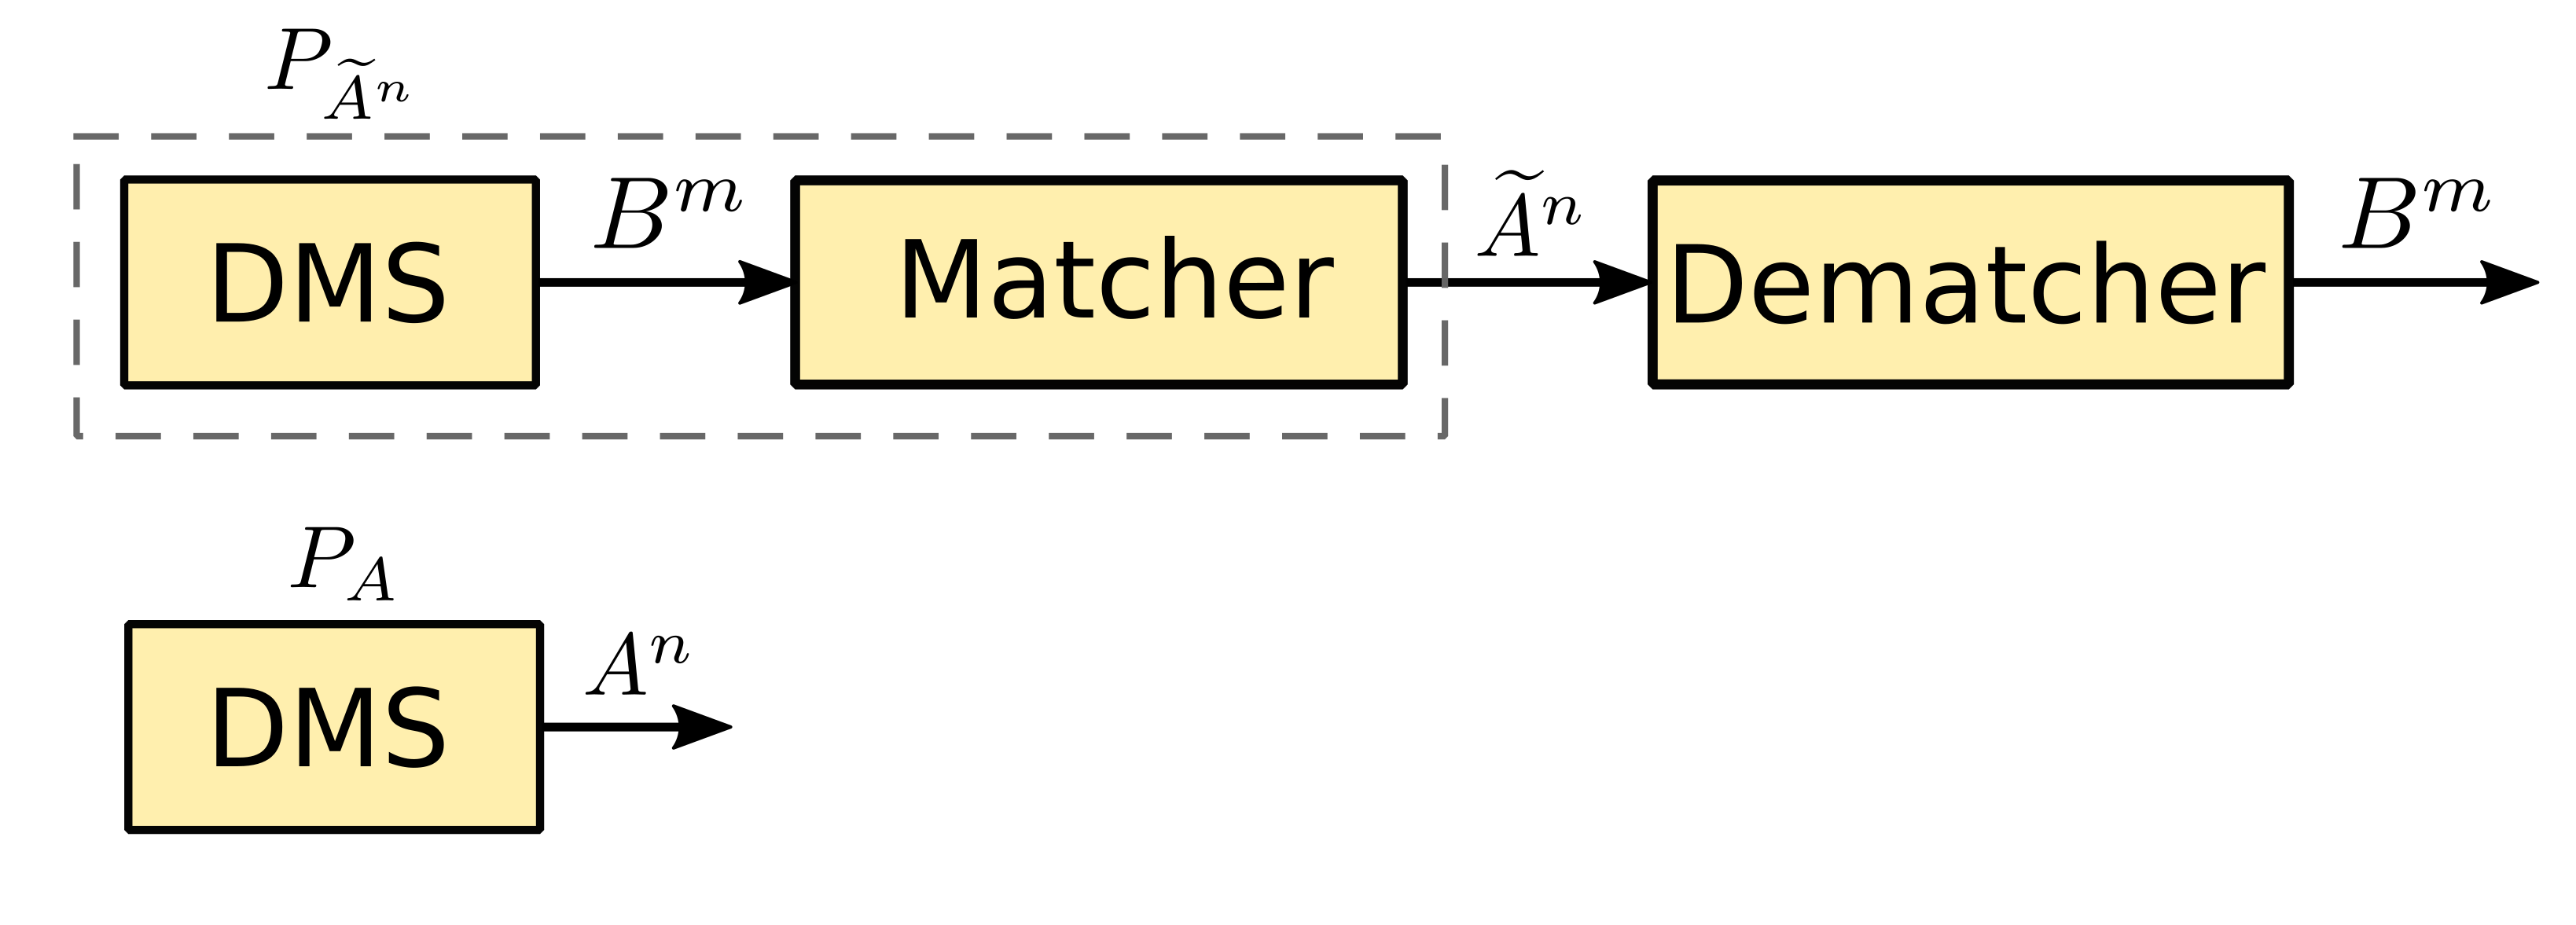
\includegraphics[width=0.70\paperwidth]{Diagramas/matcher.png}
    \end{figure}
\end{frame}


\section{Desarrollo}
\subsection{Investigación}

\begin{frame}
  \frametitle{\textbf{Tabla de Contenidos}}
  \begin{center}
    {\vspace{-1.5cm}\Large \textbf{Sección \thesection: \secname }\vspace{0.5cm}}
    \begin{beamercolorbox}[
      sep=8pt,center]{part title}
      \usebeamerfont{part title}
      \textbf{\subsecname}
    \end{beamercolorbox}
  \end{center}
\end{frame}


\begin{frame}
  \frametitle{\textbf{Flujo de trabajo}}
      \framesubtitle{\secname : \subsecname}

  \vspace{-0.3cm}
  \begin{figure}[!t] \centering
  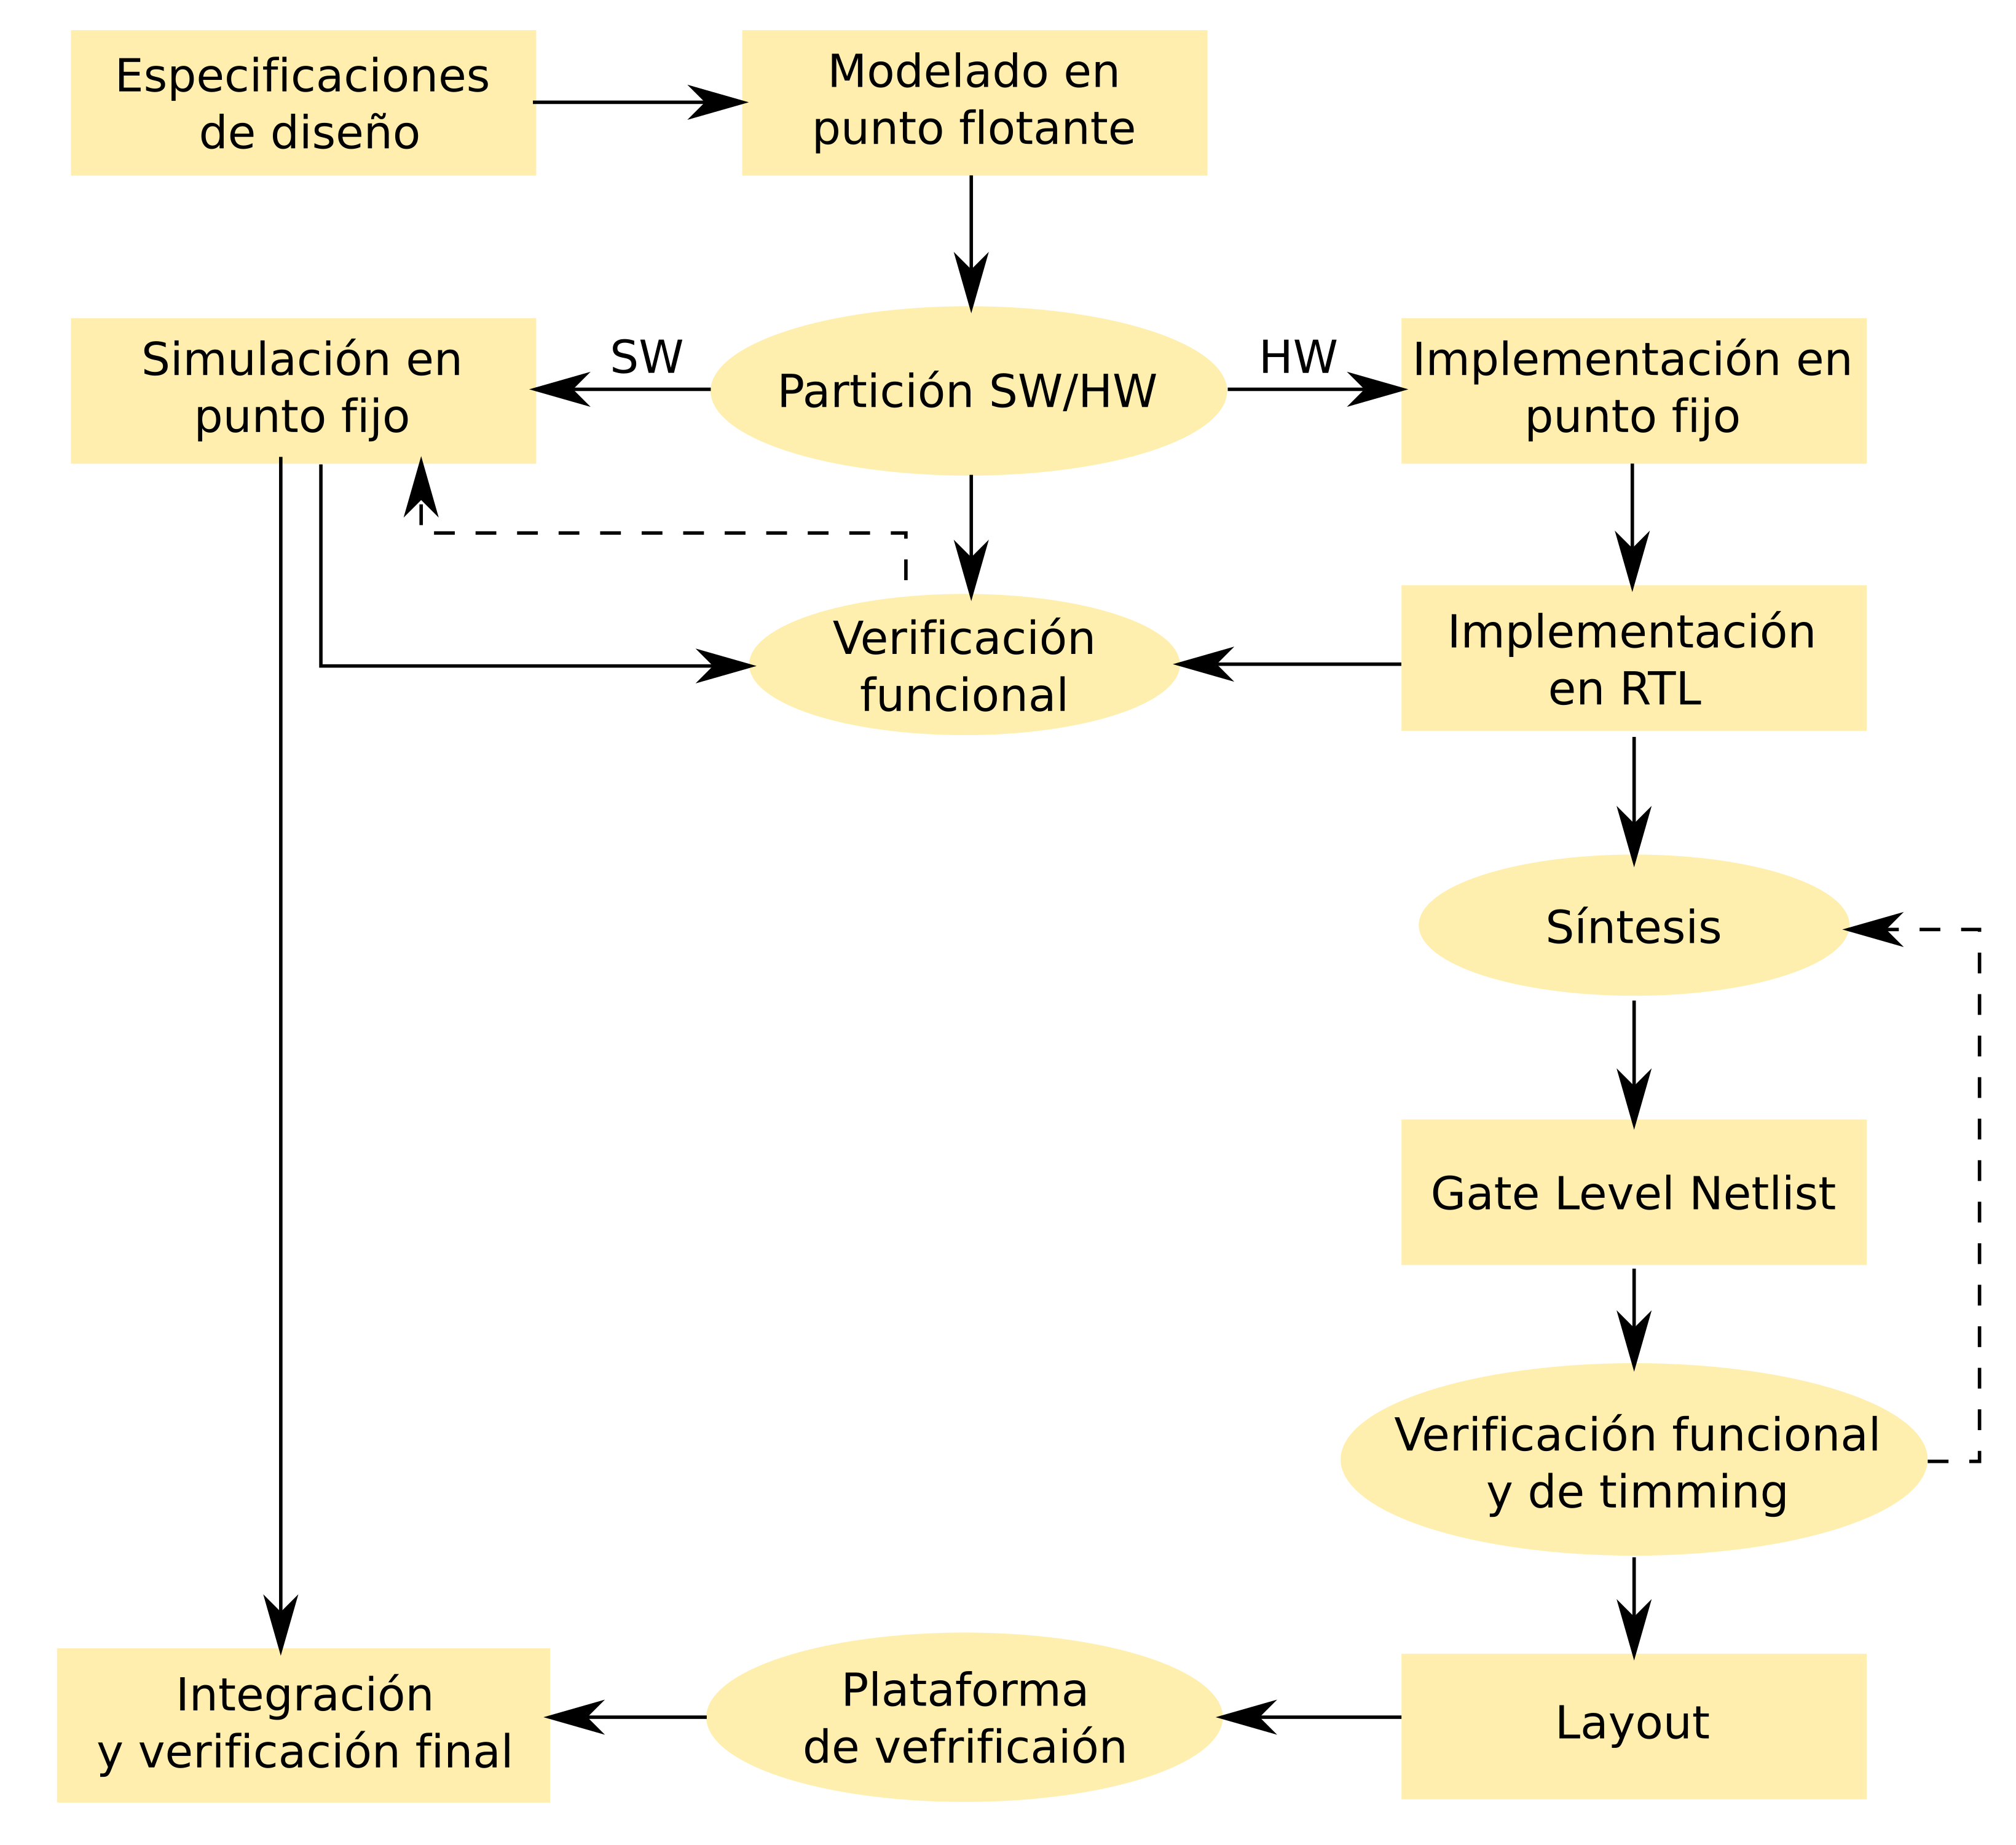
\includegraphics[width=0.65\paperwidth]{Diagramas/diag_flujo.png}
  \end{figure}
\end{frame}



\begin{frame}
  \frametitle{\textbf{Especificaciones y tipos de algoritmos}}
\framesubtitle{\secname : \subsecname}

\begin{block}{\centering \textbf{Especificaciones de diseño}}
    \begin{itemize}\Small
        \item A partir de un DMS con distribución $ P_{(x=0)}= P_{(x=1)}=0.5$ obtener una distribución con una probabilidad de ceros de $P_{(x=0)}= 0.75$.
        \item La secuencia de entrada al codificador deberá ser de 4 bits.
        \item Implementar el mismo con una modulación QAM-16.
    \end{itemize}
\end{block}
\vspace{-0.2cm}
 \begin{block}{\centering \textbf{Tipos de algoritmos}}
     \begin{itemize}\Small
         \item  Según la longitud de la secuencia de datos:
                \begin{itemize}
                     \item Longitud variable a longitud variable (v2v).
                     \item Longitud variable a longitud fija, o viceversa (v2f o f2v).
                     \item Longitud fija a longitud fija (f2f).
                \end{itemize}
        \item   Según el modo de calculo:
                \begin{itemize}
                    \item Online, es decir, en tiempo real.
                    \item Offline, es decir, de forma precalculada.
                \end{itemize}
     \end{itemize}
     
\end{block}

\end{frame}

\begin{frame}
  \frametitle{\textbf{Selección del algoritmo a utilizar}}
     \framesubtitle{\secname : \subsecname}
   
    \begin{block}{\centering \textbf{Algoritmo a utilizar}}
        \begin{itemize}\small
        \item Se utilizará el algoritmo `Constant Composition Distribution Matching' propuesto en \cite{schulte}.
        \item El mismo trabaja con longitudes fijas (f2f) y el calculo es de tipo `online'. 
        % \item Es una técnica de complejidad relativamente baja
        \end{itemize}
    \end{block}
    \vspace{-0.2cm}

    \begin{block}{\centering \textbf{Características del algoritmo}}
        \begin{itemize}\small
            \item Utiliza 'Arithmetic Coding'.
            \item Asocia un intervalo a cada una de las posibles entradas y salidas en base a su probabilidad
            \item Realiza un mapeo de cada intervalo de entrada a un único intervalo de salida
            \item Todas las secuencias de salida tienen una composición constante de `0' y `1'.
        % Insertar imagen intervalos
        \end{itemize}
    \end{block}
\end{frame}


\begin{frame}
  \frametitle{\textbf{Análisis de la longitud de palabra de salida}}
    \framesubtitle{\secname : \subsecname}
   \begin{block}{\centering \textbf{Longitud de palabra de salida}}
        \begin{itemize}\footnotesize
            \item  Cantidad de bits de entrada
            \item La probabilidad $P_{(x=1)}$ deseada
        \end{itemize}
    \end{block}
    \vspace{-0.2cm}

    \begin{block}{\centering \textbf{Condiciones necesarias}}
        \begin{itemize}\footnotesize
            \item Se debe cumplir que:
            \begin{equation*}
            {X \choose Y} \geq 2^{k}    
            \end{equation*}
        \item Donde:
            \begin{itemize}\footnotesize
                \item [$X$:] Longitud de secuencia de salida.
                \item [$Y$:] Cantidad de bits de salida en `1'.
                \item [$k$:] Longitud de secuencia entrada. 
            \end{itemize}
        \item Además se debe mantener la relación:
            \begin{equation*}
            \frac{X}{Y} =  \frac{1}{P_{(x=1)}}  
            \end{equation*}
        \end{itemize}
    \end{block}

\end{frame}

\begin{frame}
  \frametitle{\textbf{Análisis de la longitud de palabra de salida}}
    %  \framesubtitle{\secname : \subsecname}
    \begin{block}{\centering \textbf{Longitud de salida las para especificaciones de diseño}}
    \begin{itemize}\Small
        \item Para $k=4$ y $P_{(x=1)} = 0.25$ tendremos:
            \begin{equation*}
            \frac{X}{Y} = \frac{1}{P_{(x=1)}} = 4 \implies X = 4*Y
            \end{equation*}
        \item A su vez:
            \begin{equation*} 
            {X \choose Y} \geq 16 \implies X=8 \implies \frac{X-k}{k} = 100\% 
            \end{equation*}
    \end{itemize}
    \end{block}
        \begin{block}{\centering \textbf{Ejemplos para otras especificaciones}}
        \begin{itemize}
        \item $k=16$ y $P_{(x=1)} = 0.25 \implies {24 \choose 6} \geq 2^{16} \implies \frac{X-k}{k} = 50\%$ 
        \item  $k=4$ y $P_{(x=1)} = 0.285 \implies {7 \choose 2} \geq 2^{4} \implies \frac{X-k}{k} = 75\%$
    \end{itemize}
    \end{block}
\end{frame}



\begin{frame}
  \frametitle{\textbf{Calculo de intervalo de entrada del  codificador}}
\framesubtitle{\secname : \subsecname}
   \begin{block}{Ejemplo}
   \begin{itemize}
    \item $Xi_{cod} = 1010$ y $P_{(x=0)}=0.75$: 
  \end{itemize}
  \end{block}
      \vspace{-0.3cm}
  \begin{figure}[!t] \centering
  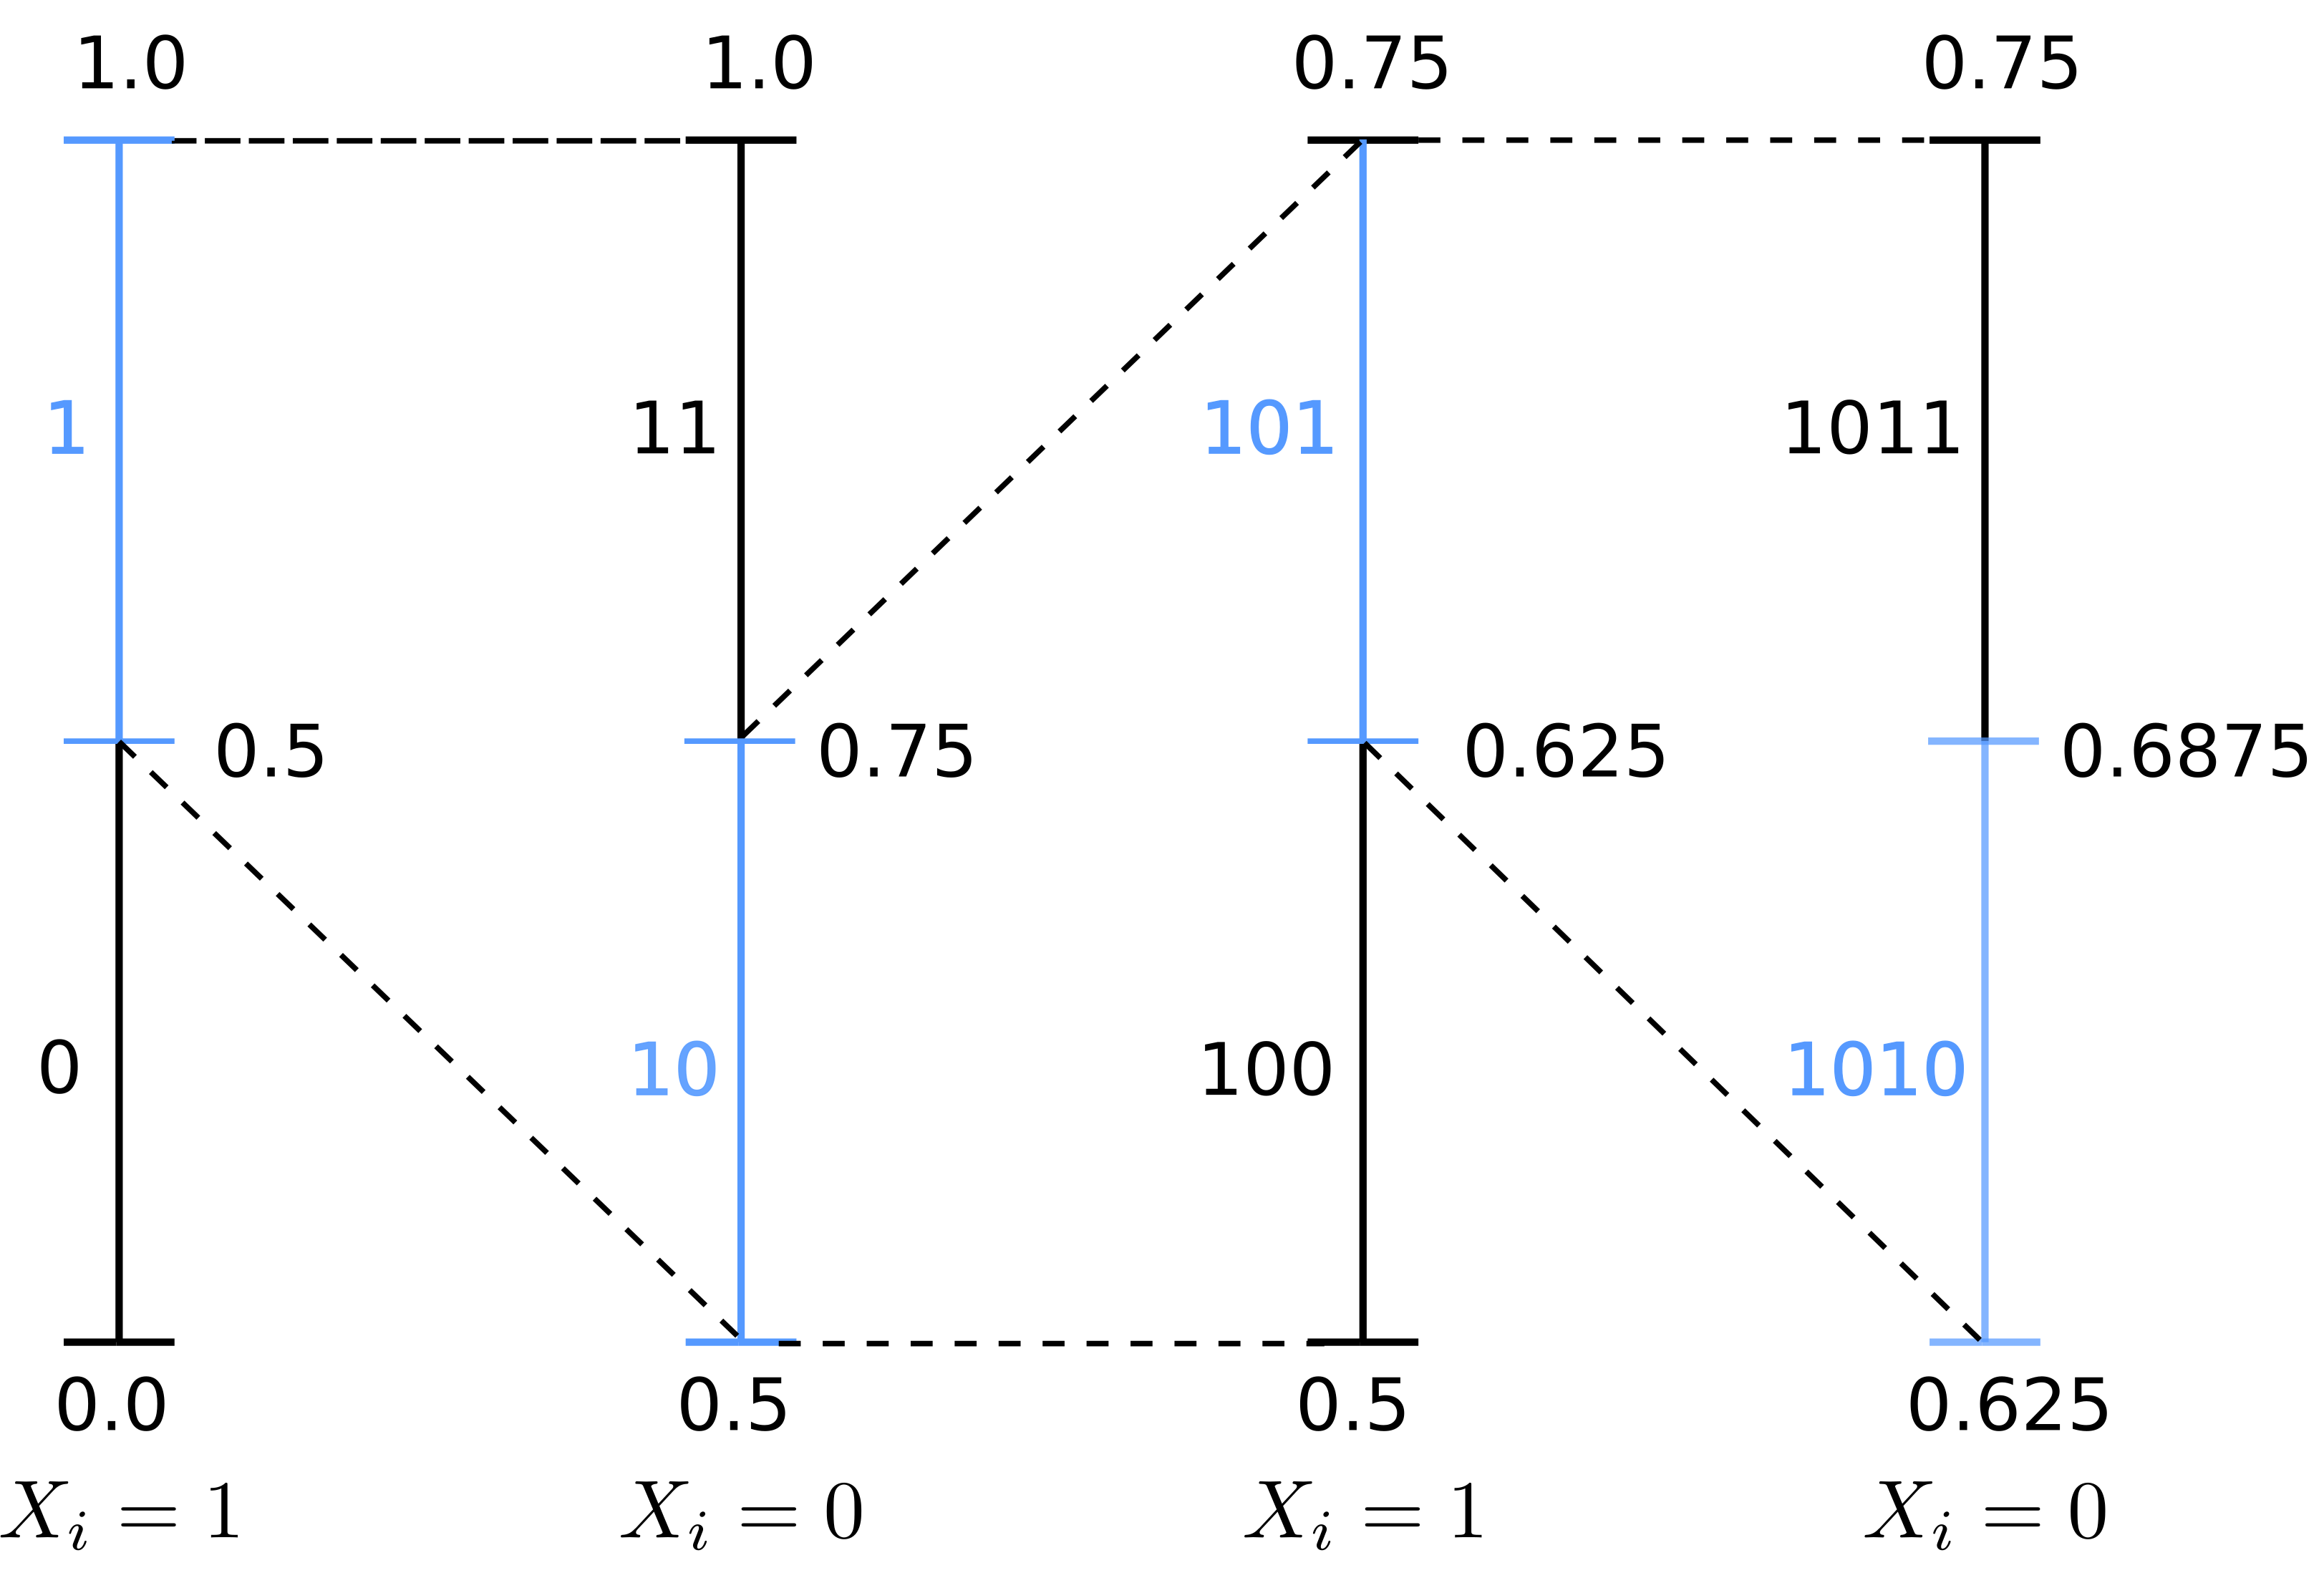
\includegraphics[width=0.80\paperheight]{Diagramas/int_ent_cod.png}%
  \end{figure}
\end{frame}

\begin{frame}
  \frametitle{\textbf{Intervalo de salida del bloque codificador}}
\framesubtitle{\secname : \subsecname}
   \begin{block}{\centering \textbf{Concepto de `Bolsa de bits'}}
   \begin{itemize}
    \item Propuesto en \cite[Sec.\ 4]{schulte}.
    \item En cada iteración se elimina un bit, obteniendo una nueva probabilidad. $P_{(x=0)}$ 
    \end{itemize}
  \end{block}
      \vspace{-0.3cm}
  \begin{figure}[!t] \centering
  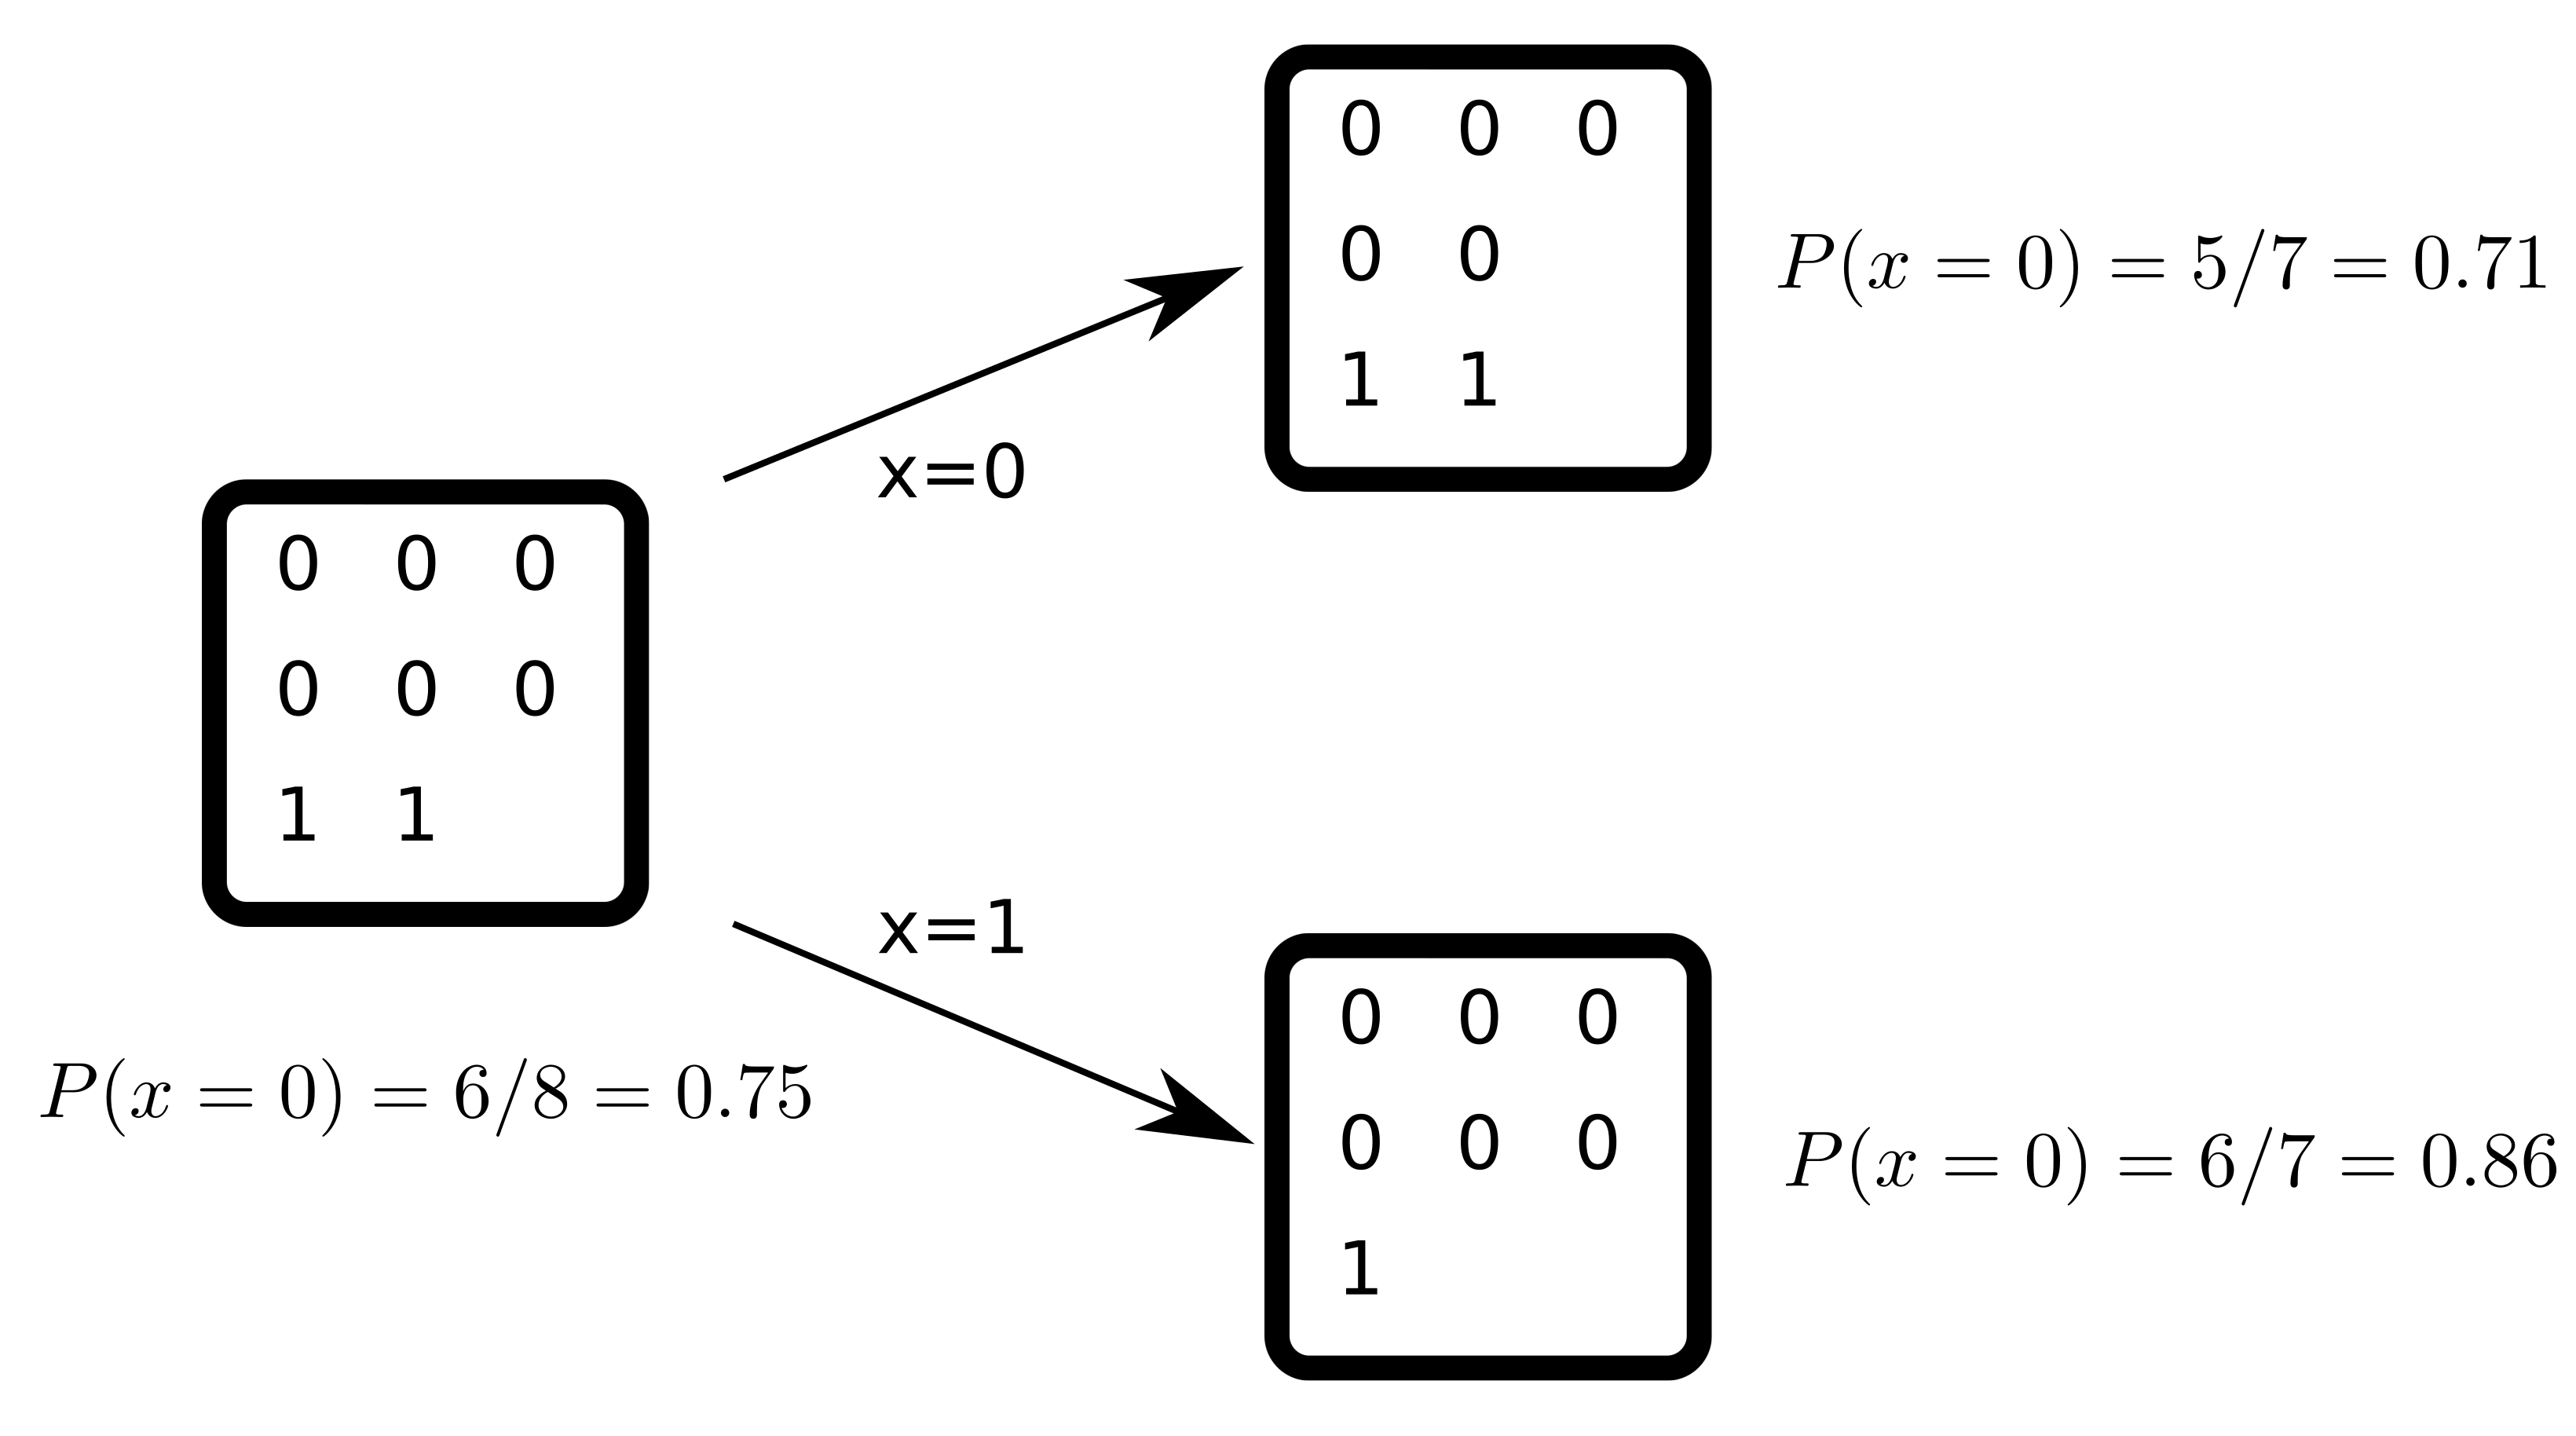
\includegraphics[width=0.70\paperwidth]{Diagramas/bag.png}%
  \end{figure}
\end{frame}

\begin{frame}
  \frametitle{\textbf{Calculo de Intervalo de salida del  codificador}}
\framesubtitle{\secname : \subsecname}
   \begin{block}{\centering \textbf{Concepto de `Escalado'}}
       \begin{itemize}\Small
            \item Propuesto en \cite[Sec.\ 4]{schulte}.
            \item Permite aumentar los límites de los subintervalos cuando estos cumplen con las siguientes condiciones:
            \begin{itemize}\footnotesize
                \item Si $u_s \leq 0.5$:
                    \begin{itemize}
                        \item $u_s' = 2  u_s$
                        \item $l_s' = 2 l_s$
                        \item $l_i' = 2  l_i$
                    \end{itemize}
                \item Si $l_s > 0.5$: 
                    \begin{itemize}
                        \item $u_s' = 2  (u_s - 0.5)$
                        \item $l_s' = 2  (l_s - 0.5)$
                        \item $l_i' = 2  (l_i - 0.5)$
                    \end{itemize}
            \end{itemize}
            \item Esto permitirá optimizar la cantidad de bits en la implementación.
        \end{itemize}
  \end{block}
\end{frame}


\begin{frame}
  \frametitle{\textbf{Calculo de intervalo de salida del bloque codificador}}
\framesubtitle{\secname : \subsecname}
   \begin{block}{Ejemplo}
   \begin{itemize}
    \item $Xi_{cod} = 1010$ y $P_{(x=0)}=0.75$: 
  \end{itemize}
  \end{block}
      \vspace{-0.3cm}
  \begin{figure}[!t] \centering
  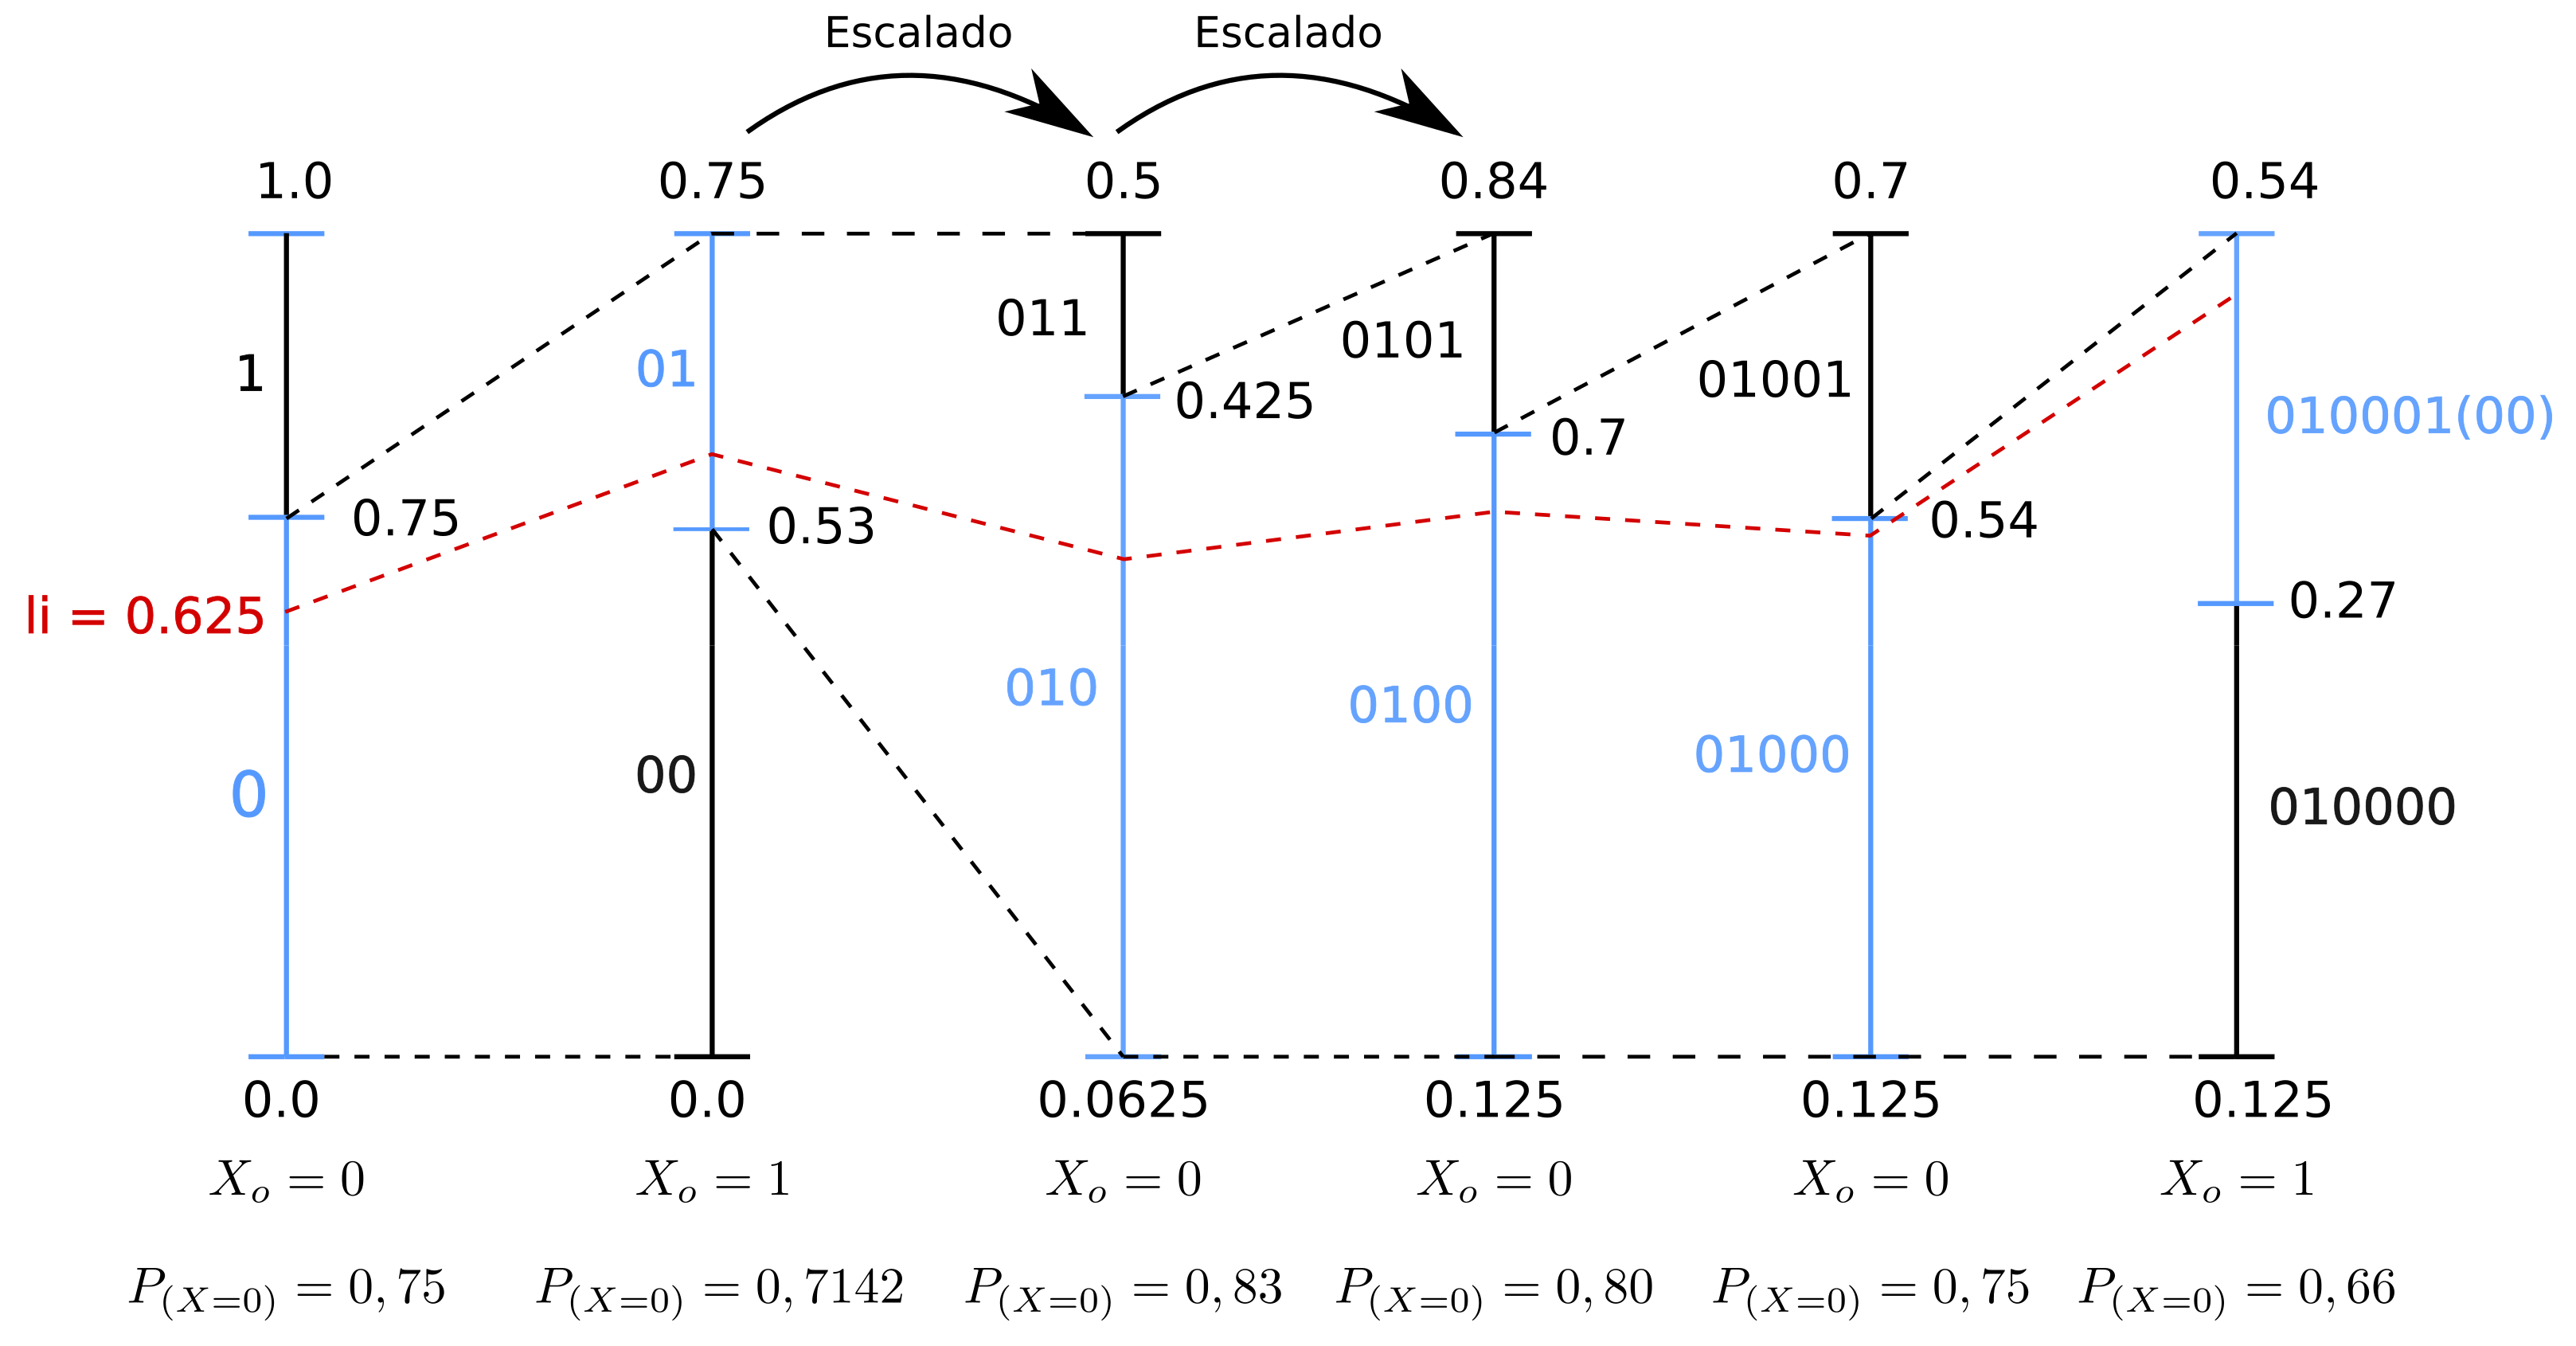
\includegraphics[width=0.85\paperwidth]{Diagramas/int_sal_cod.png}%
  \end{figure}
\end{frame}


\begin{frame}
  \frametitle{\textbf{Calculo de intervalo de entrada del  decodificador}}
\framesubtitle{\secname : \subsecname}
   \begin{block}{Ejemplo}
   \begin{itemize}
    \item $Xi_{cod} = 01000100$ y  $P_{(x=0)}=0.75$:
  \end{itemize}
  \end{block}
      \vspace{-0.3cm}
  \begin{figure}[!t] \centering
  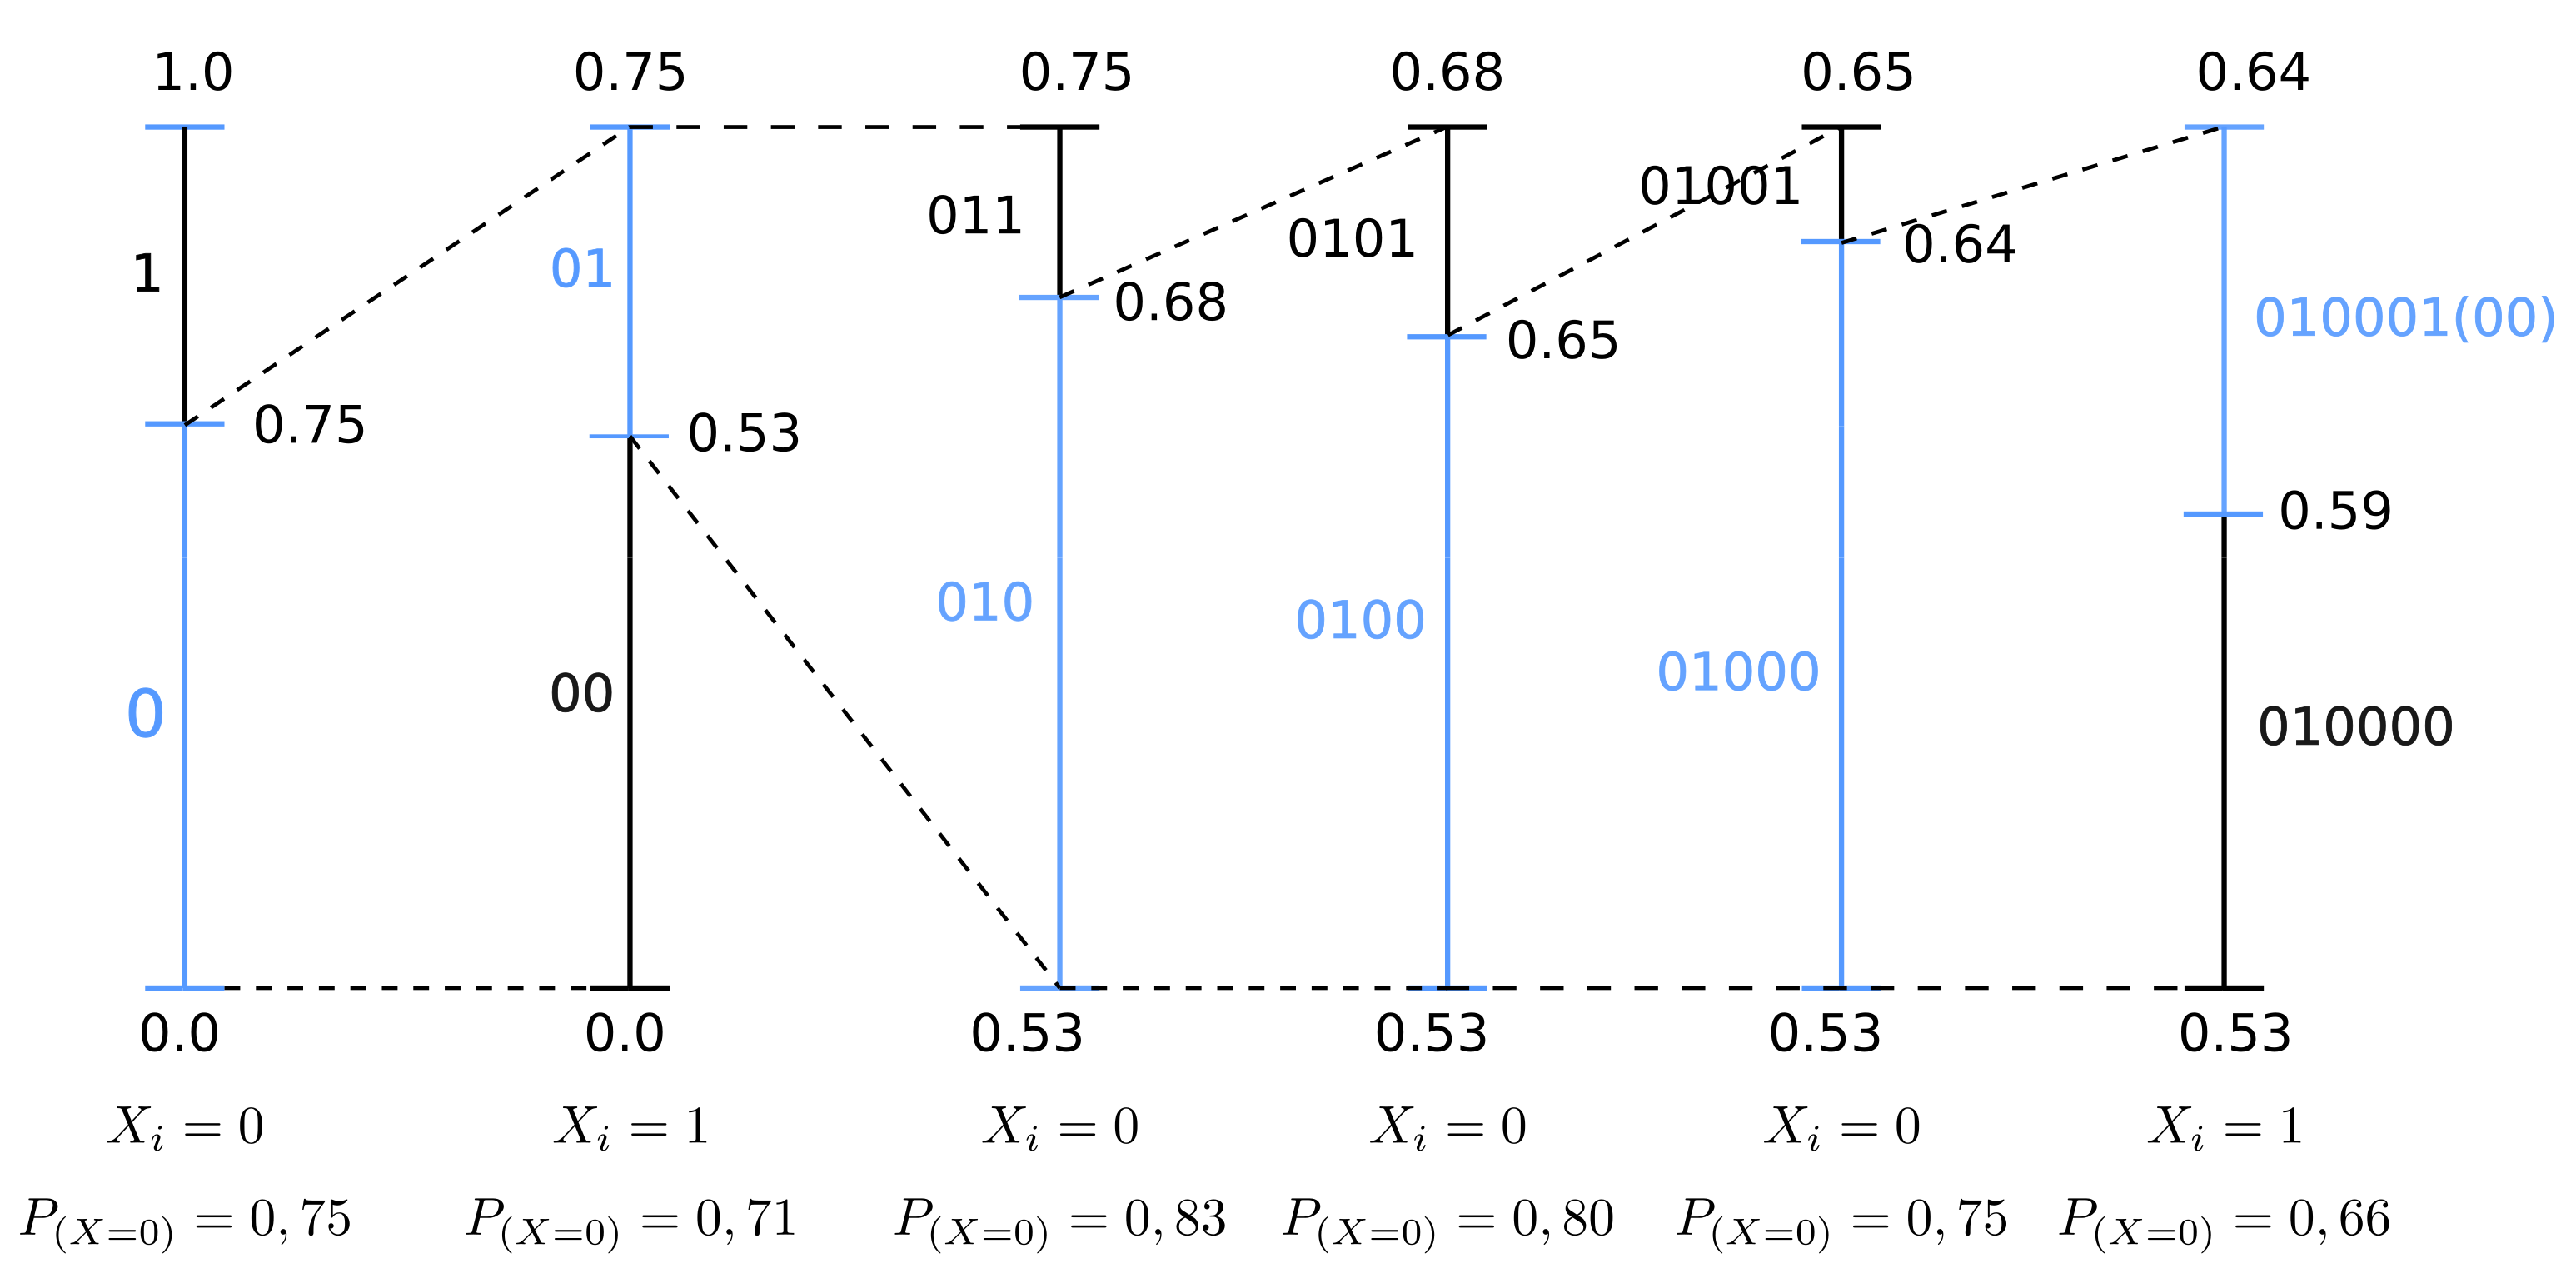
\includegraphics[width=0.85\paperwidth]{Diagramas/int_ent_dec.png}%
  \end{figure}
\end{frame}

\begin{frame}
  \frametitle{\textbf{Calculo de intervalo de salida del  decodificador}}
\framesubtitle{\secname : \subsecname}
   \begin{block}{Ejemplo}
   \begin{itemize}
    \item $Xi_{cod} = 01000100$ y  $P_{(x=0)}=0.75$:
  \end{itemize}
  \end{block}
      \vspace{-0.3cm}
  \begin{figure}[!t] \centering
  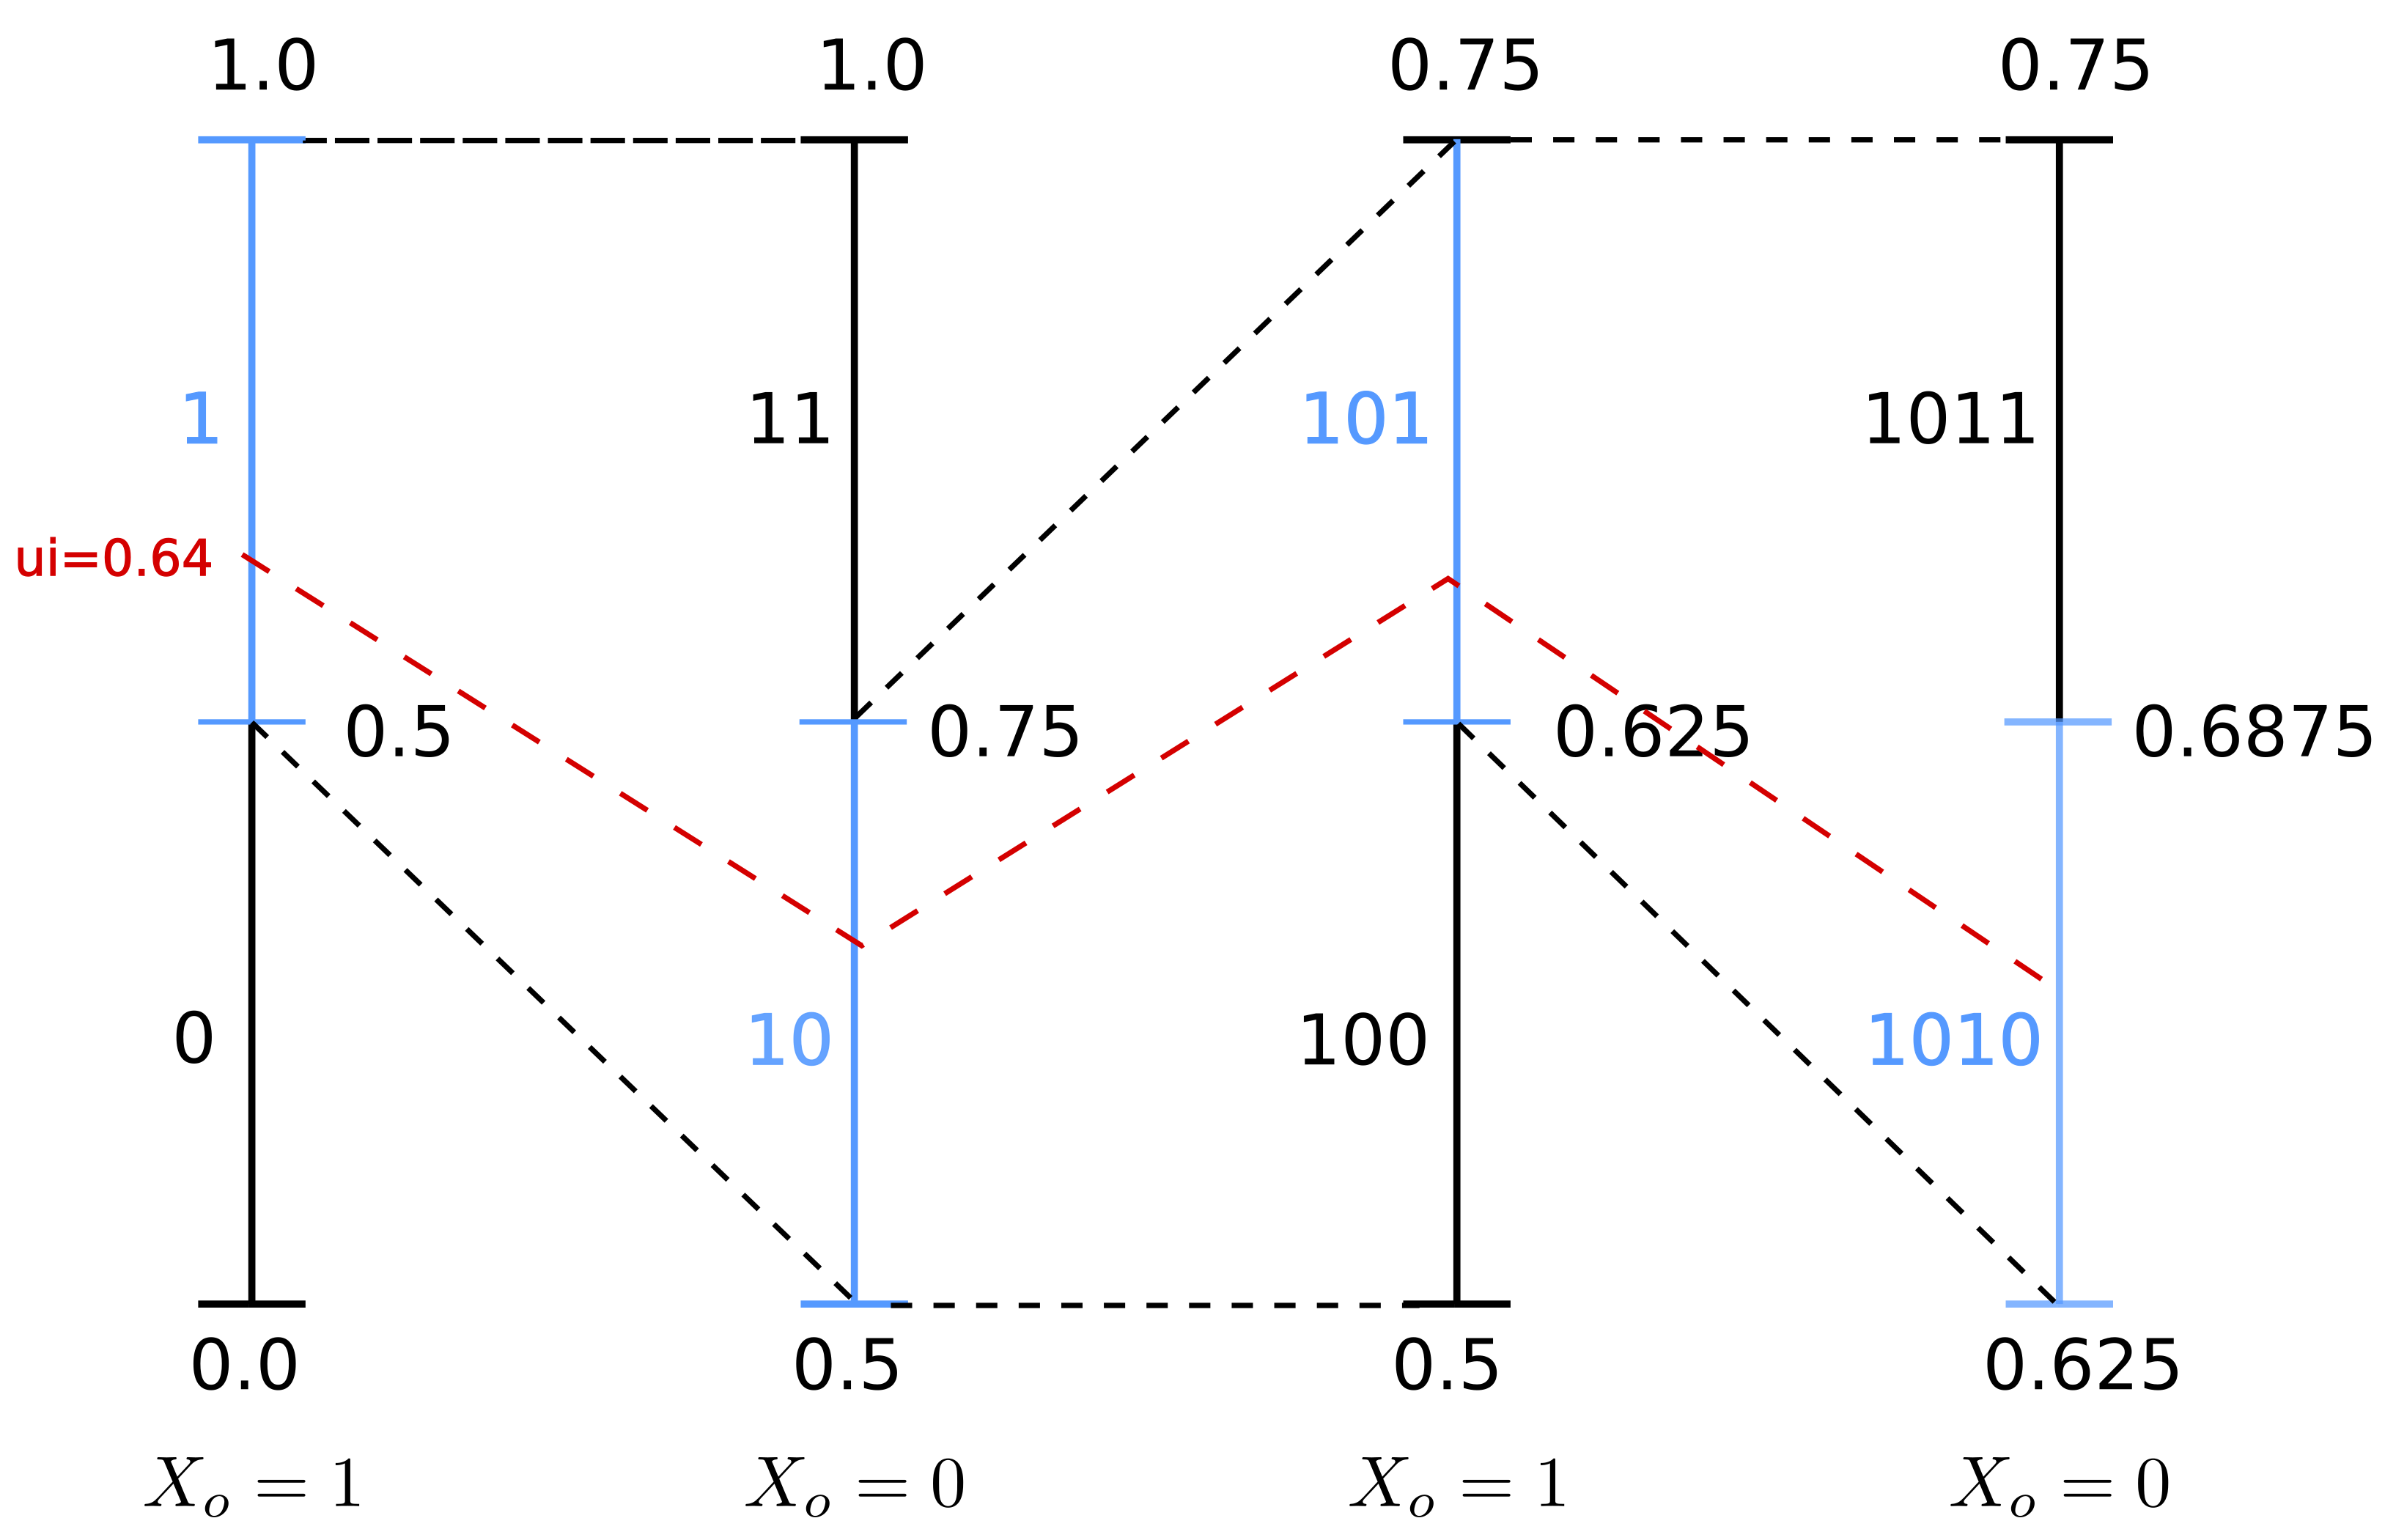
\includegraphics[width=0.70\paperwidth]{Diagramas/int_sal_dec.png}%
  \end{figure}
\end{frame}



   % Introducción y desarrollo del algoritmo
%%%%%%%%%%%%%%%%%%%%%%%%%%%%%%%%%%%%%%%%%%%%%%%%%%%%%%%%%%%%%%%%%%% 
%% Desarrollo -  Modelado en punto flotante
%%%%%%%%%%%%%%%%%%%%%%%%%%%%%%%%%%%%%%%%%%%%%%%%%%%%%%%%%%%%%%%%%%%
\subsection{Modelo en punto flotante}
\begin{frame}
  \frametitle{\textbf{Tabla de Contenidos}}
  \begin{center}
    {\vspace{-1.5cm}\Large \textbf{Sección \thesection: \secname }\vspace{0.5cm}}
    \begin{beamercolorbox}[
      sep=8pt,center]{part title}
      \usebeamerfont{part title}
      \textbf{\subsecname}
    \end{beamercolorbox}
  \end{center}
\end{frame}

\begin{frame}
  \frametitle{\textbf{Esquema de simulación}}
\framesubtitle{\secname : \subsecname}
    % \vspace{-0.3cm}

  \begin{figure}[!t] \centering
    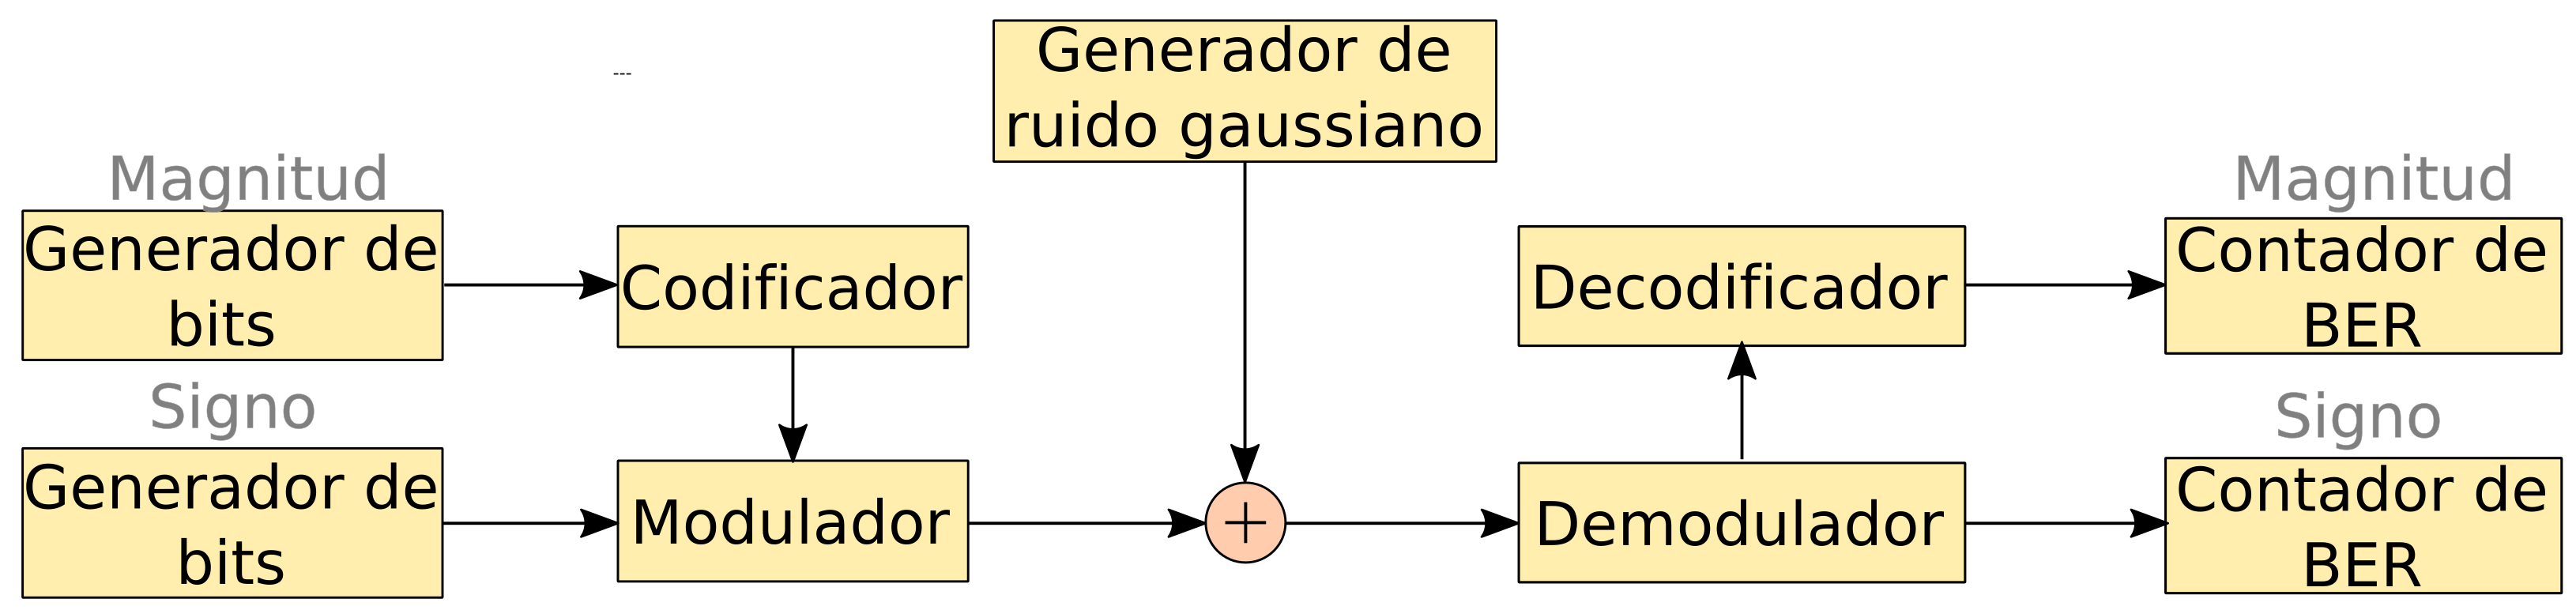
\includegraphics[width=0.85\paperwidth]{Diagramas/proyect_alto_nivel.png}%
  \end{figure}
  
  \vspace{-0.5cm}
  \noindent\rule{8cm}{0.4pt}\centering
  \vspace{-0.3cm}

  \begin{columns}
    \begin{column}{0.48\linewidth}  
        \begin{figure}
        \centering
        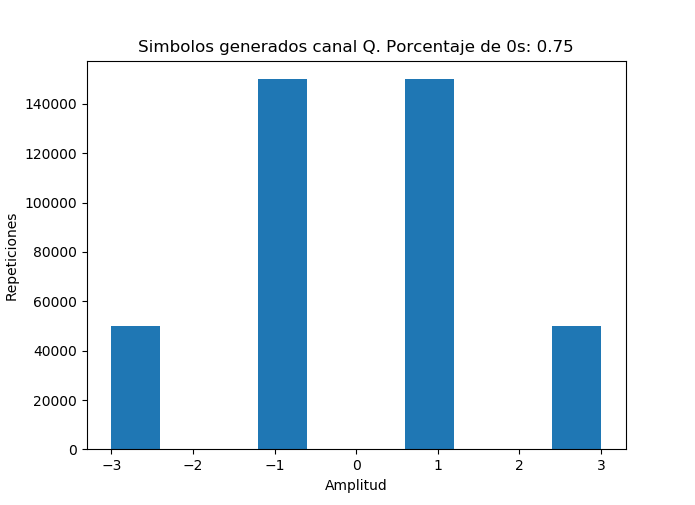
\includegraphics[width=\textwidth]{Graficos/coded_symbols_6.png}
        \end{figure}
    \end{column}
    \begin{column}{0.408\linewidth}
        \vspace{0.15cm}
        \begin{figure}
            \centering
            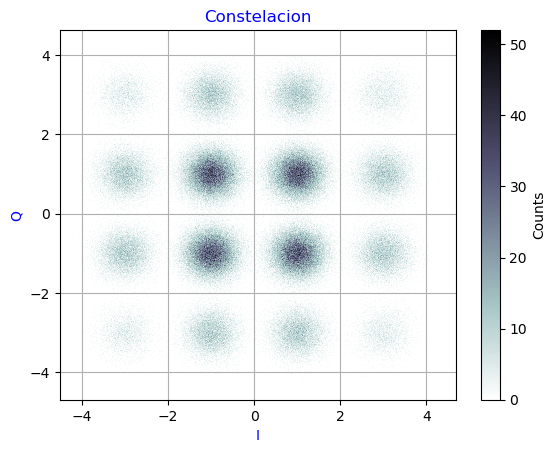
\includegraphics[width=\textwidth]{Graficos/Constellation_025.png}
        \end{figure}
    \end{column}
\end{columns}
  
\end{frame}

% \begin{frame}
%   \frametitle{\textbf{Resultados obtenidos}}
\framesubtitle{\secname : \subsecname}
% \begin{columns}
%     \begin{column}{0.48\paperwidth}  
%     \begin{figure}
%         \centering
%         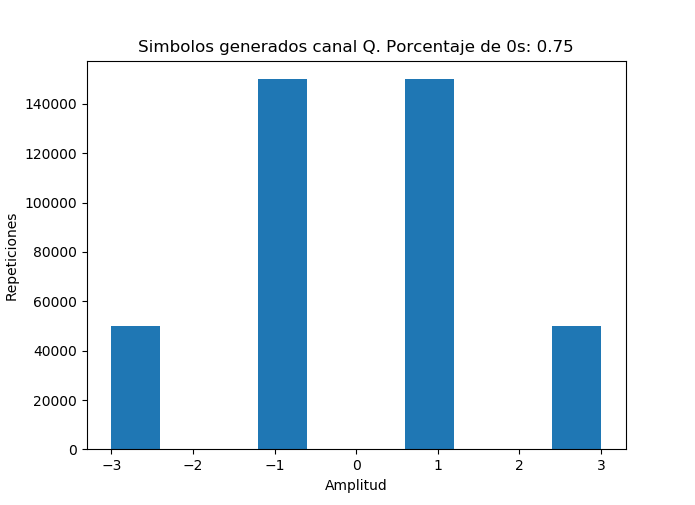
\includegraphics[width=\textwidth]{Graficos/coded_symbols_6.png}
%         \caption{Símbolos codificados, $P_{(x=0)}=0.75$}
%         %\label{fig:my_label}
%     \end{figure}
%     \end{column}

%     \begin{column}{0.48\paperwidth}
%     \begin{figure}
%         \centering
%         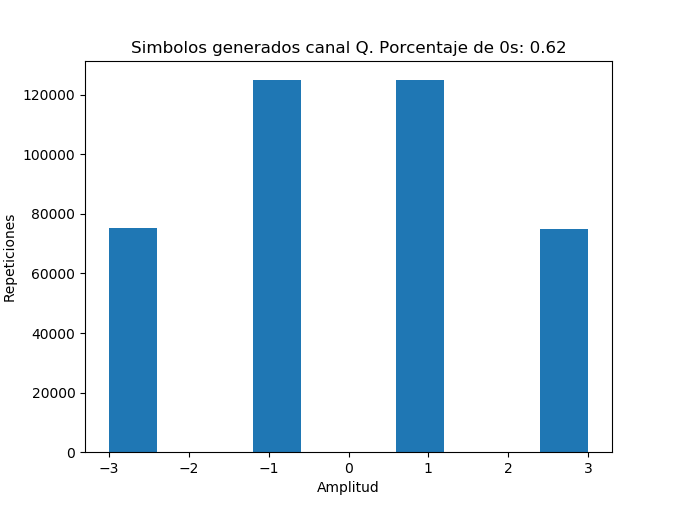
\includegraphics[width=\textwidth]{Graficos/coded_symbols_5.png}
%         \caption{Símbolos codificados, $P_{(x=0)}=0.62$}
%         % \label{fig:my_label}
%     \end{figure}
%     \end{column}
            
% \end{columns}
% \end{frame}

% \begin{frame}
%   \frametitle{\textbf{Resultados obtenidos}}
% \framesubtitle{\secname : \subsecname}
% %   Símbolos codificados, $P_{(x=0)}=0.75$
% %     \vspace{-0.3cm}

% \begin{columns}
%     \begin{column}{0.48\linewidth}  
%     \begin{figure}
%         \centering
%  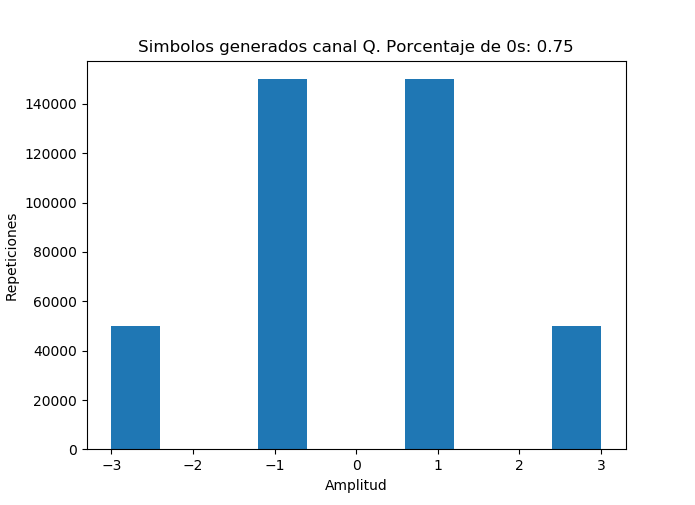
\includegraphics[width=\textwidth]{Graficos/coded_symbols_6.png}
%     \end{figure}
%     \end{column}

%     \begin{column}{0.43\linewidth}
%     \begin{figure}
%         \centering
%         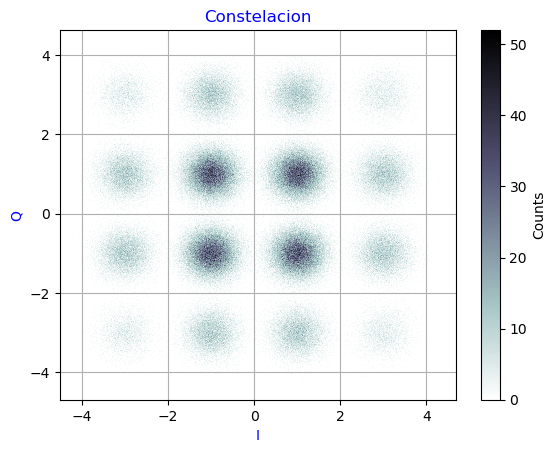
\includegraphics[width=\textwidth]{Graficos/Constellation_025.png}
%     \end{figure}
%     \end{column}
% \end{columns}
% \end{frame}


% \begin{frame}
%   \frametitle{\textbf{Resultados obtenidos}}
%\framesubtitle{\secname : \subsecname}
%   Sin realizar codificación:
% \begin{columns}
%     \begin{column}{0.48\paperwidth}  
%     \begin{figure}
%         \centering
%         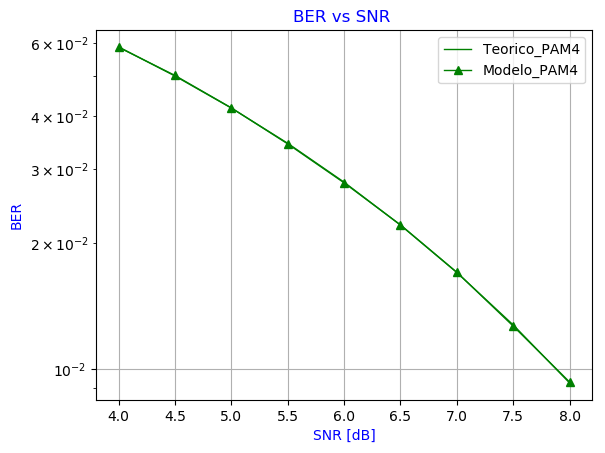
\includegraphics[width=\textwidth]{Graficos/BER_vs_SNR_1.png}%
%     \end{figure}
%     \end{column}

%     \begin{column}{0.48\paperwidth}
%     \begin{figure}
%         \centering
%         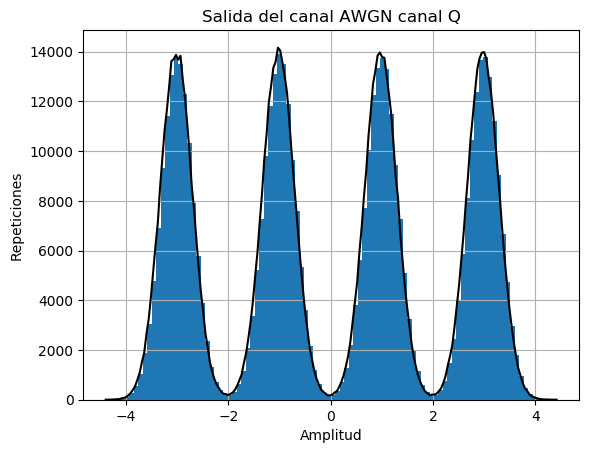
\includegraphics[width=\textwidth]{Graficos/AWGN_symbols.png}
%     \end{figure}
%     \end{column}
% \end{columns}
% \end{frame}

\begin{frame}
  \frametitle{\textbf{Penalidad por redundancia}}
\framesubtitle{\secname : \subsecname}
   \begin{block}{}
    \begin{itemize}
    \item De los 16 bits transmitidos solo 12 son de información.
    \item Se produce un desplazamiento en la curva dado por la ecuación $ 10.log(16/12)\approx1,25\, dB$
    \item Esto se conoce como `Overhead' (OH).
    \end{itemize}
    \end{block}
       \vspace{-0.3cm}
    \begin{figure}
      \centering
      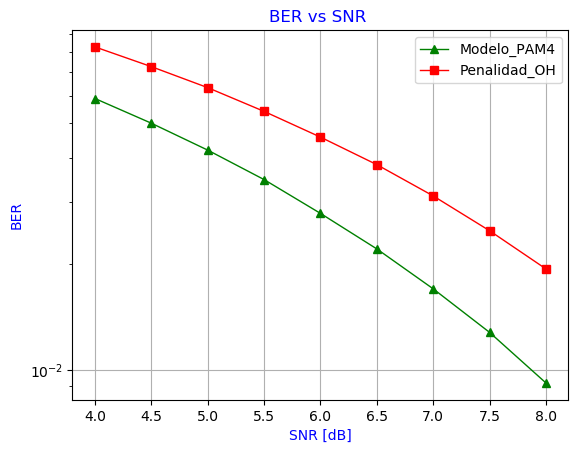
\includegraphics[width=0.50\paperwidth]{Graficos/BER_vs_SNR_2.png}%
    \end{figure}
\end{frame}

\begin{frame}
  \frametitle{\textbf{Ganancia por potencia}}
\framesubtitle{\secname : \subsecname}
   \begin{block}{}
    \begin{itemize}
    \item La potencia transmitida está dada por:
        \begin{equation*}
            P_{tx} = P_{(s = 1)}  (1)^{2} + P_{(s = 3)}  (3)^{2}
        \end{equation*}
    \item Para $ P_{(s = 3)}=0.25$ se obtiene una reducción de potencia del 40\% respecto a $ P_{(s = 3)}=0.50$.
    % \item SNR constante. 
    \end{itemize}
    \end{block}
     \vspace{-0.3cm}

   \begin{figure}
  \centering
  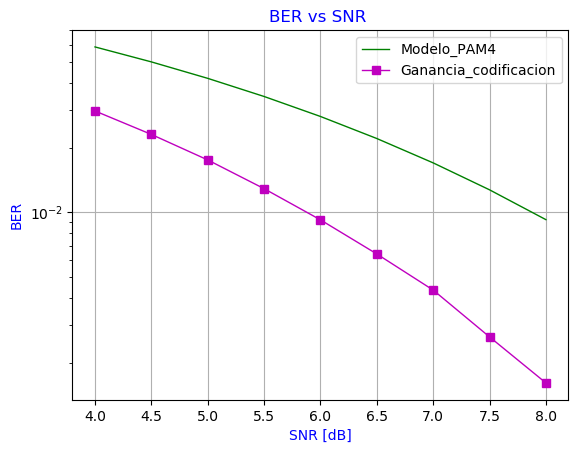
\includegraphics[width=0.45\paperwidth]{Graficos/BER_vs_SNR_3.png}%
\end{figure}
\end{frame}


\begin{frame}
  \frametitle{\textbf{Multiplicación de errores}}
\framesubtitle{\secname : \subsecname}
      \begin{block}{}

   \begin{itemize}\small
    \item Un error de un bit transmitido puede verse reflejado en hasta 4 bits a la salida
 del decodificador.
 \item Considerando este efecto, el sistema presenta un mejor desempeño que una modulación PAM-4 para una SNR mayor a 7dB.
 \end{itemize}
 \end{block}
     \vspace{-0.3cm}

\begin{columns}
    \begin{column}{0.65\paperwidth}
    \begin{figure}
        \centering
        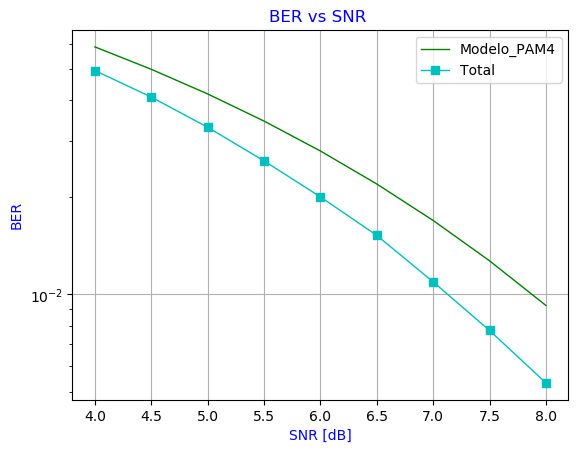
\includegraphics[width=0.45\textwidth]{Graficos/BER_vs_SNR_4.png}%
        \label{fig:my_label}
    \end{figure}

    \end{column}
    \begin{column}{0.65\paperwidth}  
    
    \begin{figure}
        \centering
        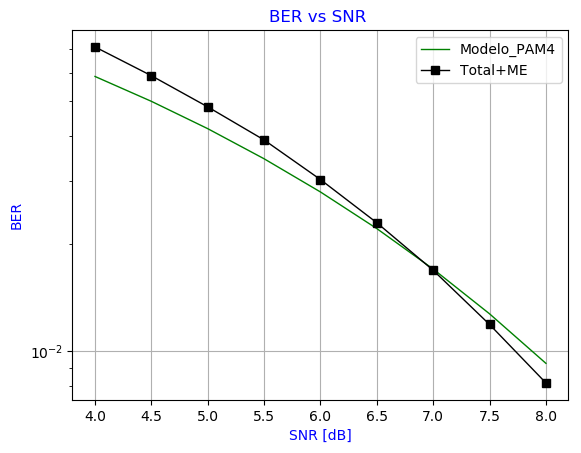
\includegraphics[width=0.45\textwidth]{Graficos/BER_vs_SNR_5.png}
        \label{fig:my_label}
    \end{figure}
    
    \end{column}
\end{columns}
\end{frame}

\begin{frame}
  \frametitle{\textbf{Modelo final}}
\framesubtitle{\secname : \subsecname}
      \begin{block}{}
        % \begin{itemize}
        %     \item Disminución de potencia
        %     \item Penalidad por redundancia 
        %  \end{itemize}
        \begin{itemize}
            \item Comparación con QAM8. 
            \item Secuencia de entrada de 100 bits.
            \item Probabilidad de $P_{(s=3)} = 0.12$.
     \end{itemize}  
     \end{block}
    \vspace{-0.3cm}

\begin{columns}
    % \begin{column}{0.48\paperwidth}
    % \begin{figure}
    %     \centering
    %     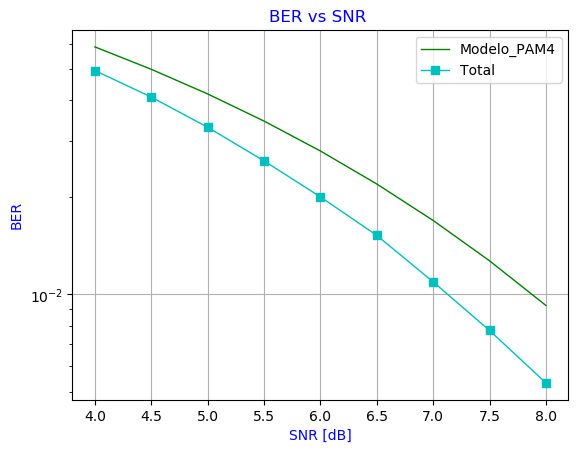
\includegraphics[width=\textwidth]{Graficos/BER_vs_SNR_4.png}%
    %     \label{fig:my_label}
    % \end{figure}
    % \end{column}
    
    \begin{column}{0.48\paperwidth}  
    \begin{figure}
        \centering
        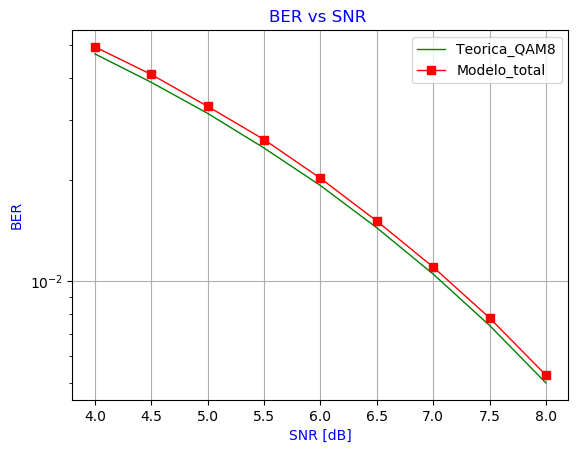
\includegraphics[width=\textwidth]{Graficos/BER_vs_SNR_6.png}
        \label{fig:my_label}
    \end{figure}
    \end{column}
    
    \begin{column}{0.48\paperwidth} 
        \begin{figure}
          \centering
          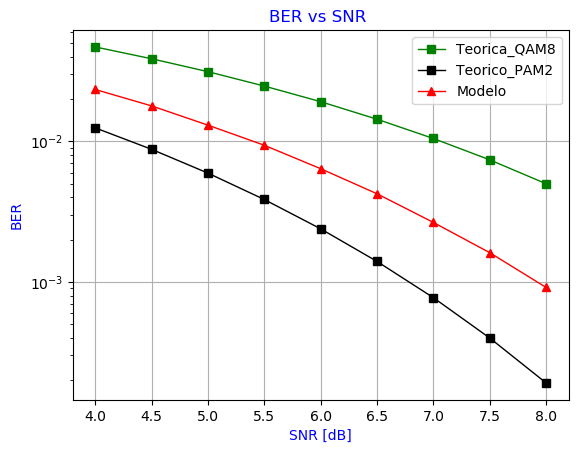
\includegraphics[width=\textwidth]{Graficos/BER_vs_SNR_8.png}%
        \end{figure}
        \end{column}
    \end{columns}

\end{frame}

% \begin{frame}
%   \frametitle{\textbf{Modelo final}}
%      \framesubtitle{\secname : \subsecname}
%   \begin{block}{\centering \textbf{Si se considera:}}
  
%     \end{block}
%     \vspace{-0.3cm}
 
% \end{frame}


\begin{frame}
  \frametitle{\textbf{Umbral de decisión}}
\framesubtitle{\secname : \subsecname}
      \begin{block}{\centering \textbf{Umbral de decisión}}
  \begin{itemize}
    \item Mejora en el desempeño.
    \item La diferencia se reduce a medida que la SNR aumenta.  
 \end{itemize}
    \end{block}
\vspace{-0.3cm}
\begin{columns}
    \begin{column}{0.48\paperwidth}
     \begin{figure}
      \centering
      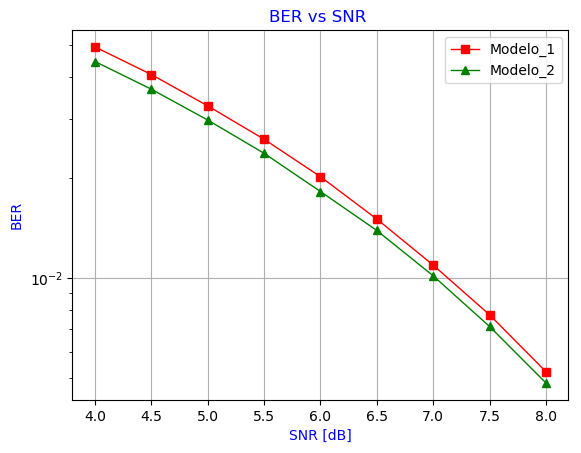
\includegraphics[width=\textwidth]{Graficos/BER_vs_SNR_9.png}%
    \end{figure}
    
    \end{column}
    \begin{column}{0.48\paperwidth}  
    \begin{figure}
        \centering
         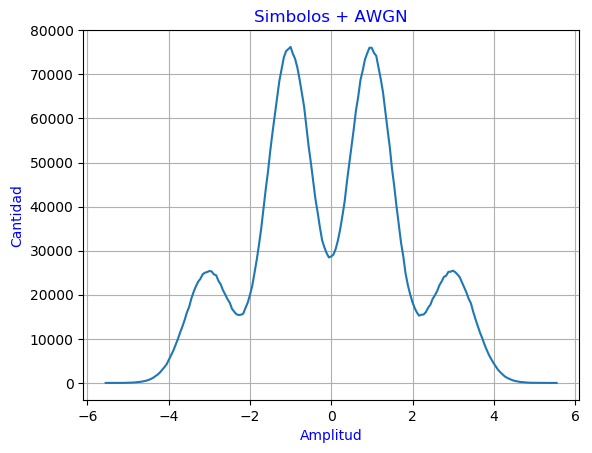
\includegraphics[width=\textwidth]{Graficos/Slicer_025.png}
    \end{figure}
   
    \end{column}
\end{columns}
\end{frame}


\begin{frame}
  \frametitle{\textbf{Umbral de decisión}}
\framesubtitle{\secname : \subsecname}
     \begin{block}{\centering \textbf{Umbral de decisión}}
     \begin{itemize}
        \item Está dado por: 
             \begin{equation*}
            P_{(s=1)}* exp{(\frac{-(\tau-1)}{2{\sigma}^{2}})} =  P_{(s=3)}* exp{(\frac{-(\tau-3)}{2{\sigma}^{2}})}
            \end{equation*}
    \item Donde:
    \begin{description}\footnotesize
    \item [$\tau:$] Umbral de decisión.
    \item [$\sigma^2:$] Varianza del ruido.
    \end{description}
    \item  Para $P_{(s=1)}=0.75$ :
        \begin{equation*}
            \tau = 2 + 0.55  *{\sigma}^{2}
        \end{equation*}
    \end{itemize}
    \end{block}
\end{frame}   % Modelado en punto flotante
%%%%%%%%%%%%%%%%%%%%%%%%%%%%%%%%%%%%%%%%%%%%%%%%%%%%%%%%%%%%%%%%%%% 
%% Desarrollo -  Modelado en punto fijo
%%%%%%%%%%%%%%%%%%%%%%%%%%%%%%%%%%%%%%%%%%%%%%%%%%%%%%%%%%%%%%%%%%%

\subsection{Modelo en punto fijo}
\begin{frame}
  \frametitle{\textbf{Tabla de Contenidos}}
  \begin{center}
    {\vspace{-1.5cm}\Large \textbf{Sección \thesection: \secname }\vspace{0.5cm}}
    \begin{beamercolorbox}[
      sep=8pt,center]{part title}
      \usebeamerfont{part title}
      \textbf{\subsecname}
    \end{beamercolorbox}
  \end{center}
\end{frame}

\begin{frame}
  \frametitle{\textbf{Consideraciones}}
   \framesubtitle{\secname : \subsecname}

    \begin{block}{\centering \textbf{Calculo de intervalos}}
    \begin{itemize}\small
    \item El calculo del intervalo de entrada se realiza a la mitad de frecuencia que el de salida en el bloque codificador, de forma inversa en el decodificador.
     \item El cálculo del intervalo de entrada y salida del codificador se realiza de manera recursiva y secuencial respectivamente.
    \item El cálculo del intervalo de entrada y salida del decodificador se realiza de forma recursiva.
    \end{itemize}
    \end{block}
    \vspace{-0.2cm}

    \begin{block}{\centering \textbf{Cuantizacion de variables}}
    Se consideran tres grupos de variables:
    \begin{itemize}\small
    \item Intervalos del codificador.
    \item Probabilidades.
    \item Intervalos del decodificador.
    \end{itemize}
    \end{block}
\end{frame}

\begin{frame}
  \frametitle{\textbf{Resoluciones de intervalos del codificador}}
      \framesubtitle{\secname : \subsecname}

    \begin{block}{}
    \begin{itemize}
    \item Se cuantizan únicamente los limites de los intervalos del codificador.
    \item La resolución elegida para este grupo de variables será U(7,6).
    \end{itemize}
    \end{block}
    \vspace{-0.3cm}
    \begin{columns}
    \begin{column}{0.48\paperwidth}
     \begin{figure}
     \centering
    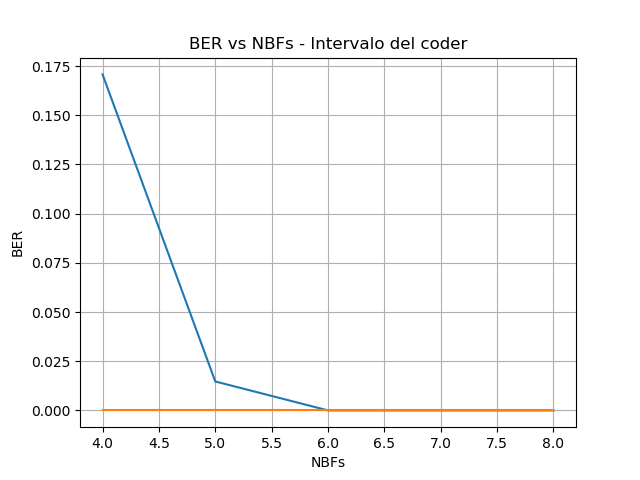
\includegraphics[width=\textwidth]{Graficos/cuantization.png}%
    \caption{Con escalado}
    \end{figure}
    \end{column}
    \begin{column}{0.48\paperwidth}  
    \begin{figure}
    \centering
    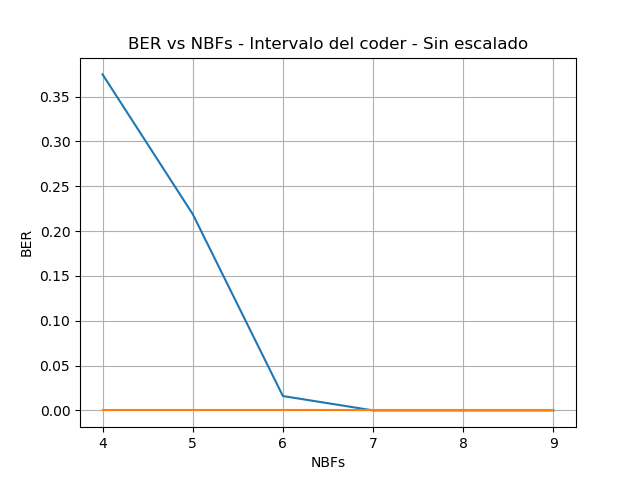
\includegraphics[width=\textwidth]{Graficos/cuantization4.png}%
    \caption{Sin escalado}
    \end{figure}
    \end{column}
\end{columns}
    \end{frame}

\begin{frame}
  \frametitle{\textbf{Resolución de probabilidades}}
\framesubtitle{\secname : \subsecname}
    \begin{block}{}
    \begin{itemize}
    \item  La resolución de los intervalos del codificador se mantiene constante.
    \item  La resolución elegida para este grupo de variables será U(5,4).
    \end{itemize}
    \end{block}
       \vspace{-0.3cm}
    \begin{columns}
    \begin{column}{0.48\paperwidth}
     \begin{figure}
     \centering
    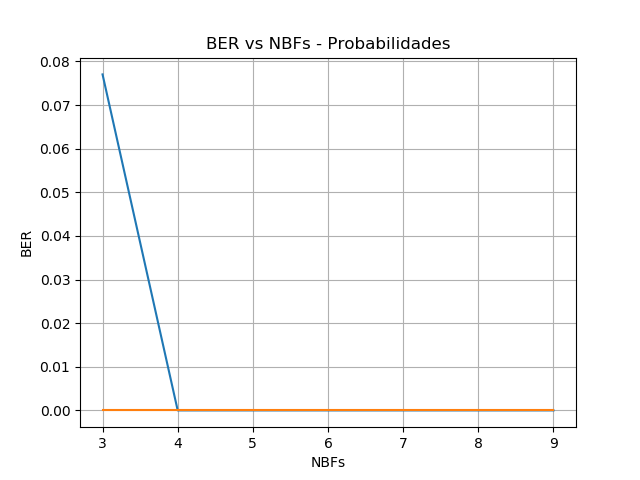
\includegraphics[width=\textwidth]{Graficos/cuantization2.png}%
    \caption{Con escalado}
    \end{figure}
    \end{column}
    \begin{column}{0.48\paperwidth}  
    \begin{figure}
    \centering
    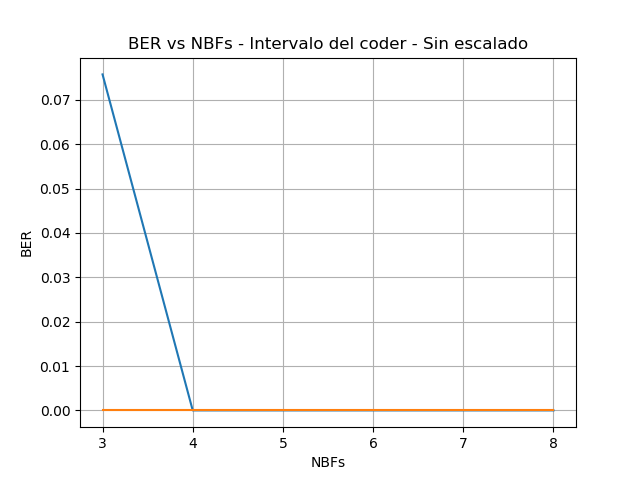
\includegraphics[width=\textwidth]{Graficos/cuantization5.png}%
    \caption{Sin escalado}
    \end{figure}
    \end{column}
\end{columns}
   \end{frame}

\begin{frame}
  \frametitle{\textbf{Resolución de intervalos del decodificador}}
\framesubtitle{\secname : \subsecname}

    \begin{block}{}
    \begin{itemize}
    \item Se mantiene constante la resolución de los intervalos del codificador y las variables de probabilidad.
    \item La resolución elegida para este grupo es U(10,9).
    \end{itemize}
    \end{block}
    \vspace{-0.3cm}
    \begin{columns}
    \begin{column}{0.48\paperwidth}
     \begin{figure}
     \centering
    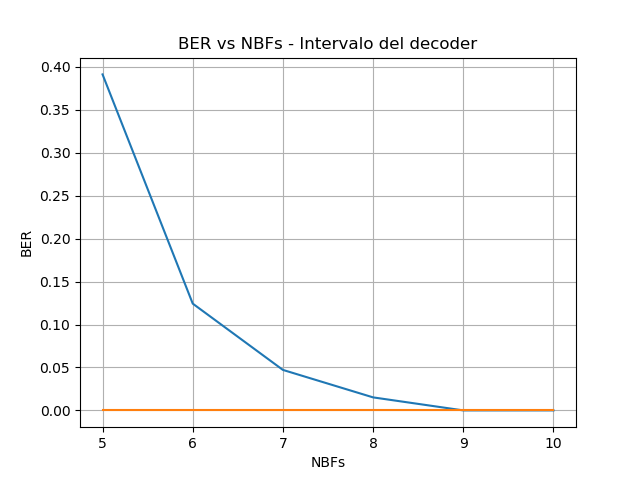
\includegraphics[width=\textwidth]{Graficos/cuantization3.png}%
    \caption{Con escalado}
    \end{figure}
    \end{column}
    \begin{column}{0.48\paperwidth}  
    \begin{figure}
    \centering
    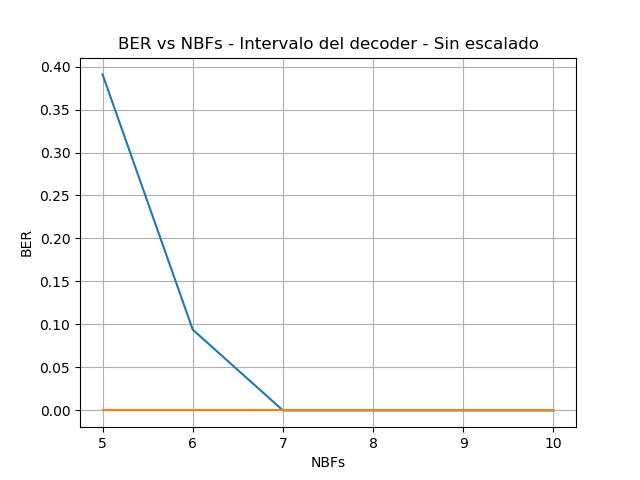
\includegraphics[width=\textwidth]{Graficos/cuantization6.png}%
    \caption{Sin escalado}
    \end{figure}
    \end{column}
\end{columns}
\end{frame}

\begin{frame}
  \frametitle{\textbf{Consideraciones finales}}
    \framesubtitle{\secname : \subsecname}

    \begin{block}{\centering \textbf{Retardos en la salida del codificador}}
     \begin{itemize}
     \item Se deben incluir de tal forma que no afecte el sincronismo de datos.
      \item Se agregó una cantidad de retardos en el canal de comunicación para que esto no sea un problema.
      \end{itemize}
     \end{block}
    \begin{block}{\centering \textbf{Ejemplo}}
    La secuencia [1,0,0,0] se codifica a [0,1,0,0,0,0,1,0], si el canal presenta un retardo, la secuencia será [1,0,0,0,1,0,0,0] y decodificacion resultara erronea. 
    \end{block}
\end{frame}



   % Modelado en punto fijo
%%%%%%%%%%%%%%%%%%%%%%%%%%%%%%%%%%%%%%%%%%%%%%%%%%%%%%%%%%%%%%%%%%% 
%% Desarrollo -  Implementación
%%%%%%%%%%%%%%%%%%%%%%%%%%%%%%%%%%%%%%%%%%%%%%%%%%%%%%%%%%%%%%%%%%%

\subsection{Implementación}
\begin{frame}
  \frametitle{\textbf{Tabla de Contenidos}}
  \begin{center}
    {\vspace{-1.5cm}\Large \textbf{Sección \thesection: \secname }\vspace{0.5cm}}
    \begin{beamercolorbox}[
      sep=8pt,center]{part title}
      \usebeamerfont{part title}
      \textbf{\subsecname}
    \end{beamercolorbox}
  \end{center}
\end{frame}


\begin{frame}
  \frametitle{\textbf{\textbf{Bloque PAM-4}}}
       \framesubtitle{\secname : \subsecname}
    \vspace{-0.3cm}
  \begin{figure}[!t] \centering
  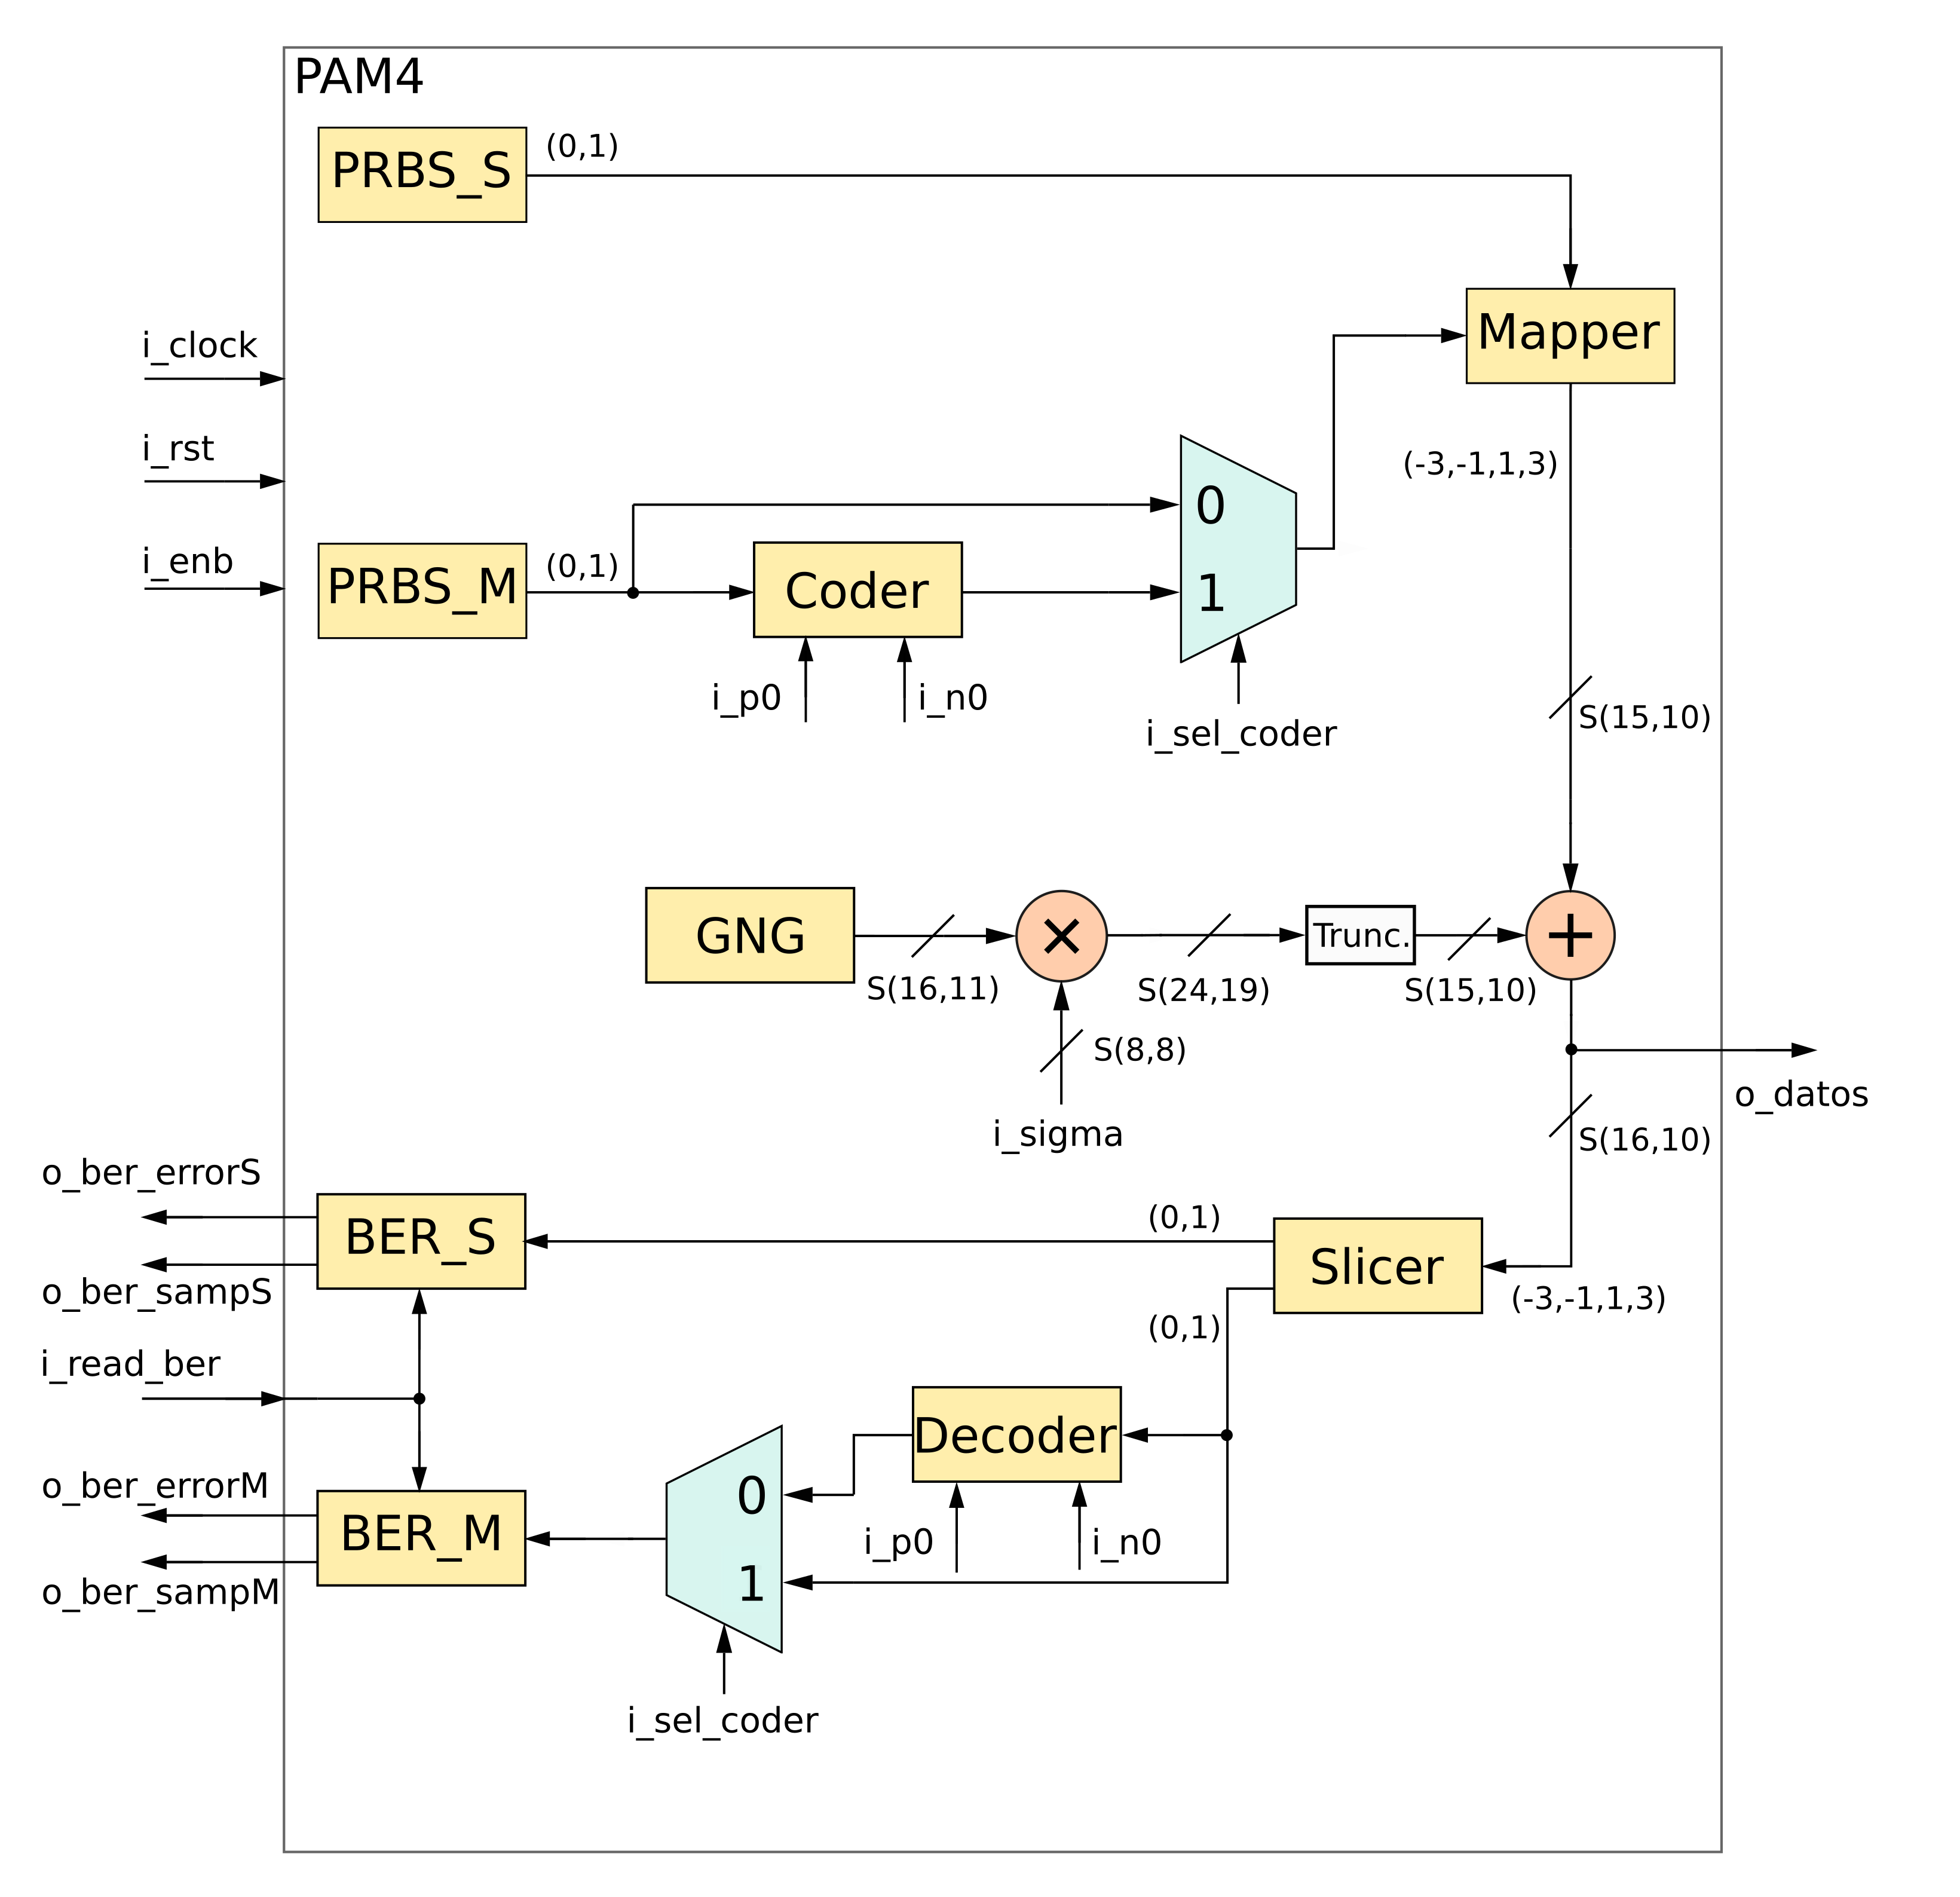
\includegraphics[ height=0.85\paperheight]{Diagramas/top_project.png}%
  \end{figure}
\end{frame}

\begin{frame}
  \frametitle{\textbf{\textbf{Bloque codificador y decodificador}}}
      \framesubtitle{\secname : \subsecname}
    \begin{block}{\centering \textbf{Estructura interna}}
    El bloque CISC se ejecuta de forma secuencial, mientras que los bloques CIEC, CIED y CISD se ejecutan de forma recursiva.
    \end{block}
    \begin{columns}
        \begin{column}{0.5\linewidth}  
        \begin{figure}
            \centering
        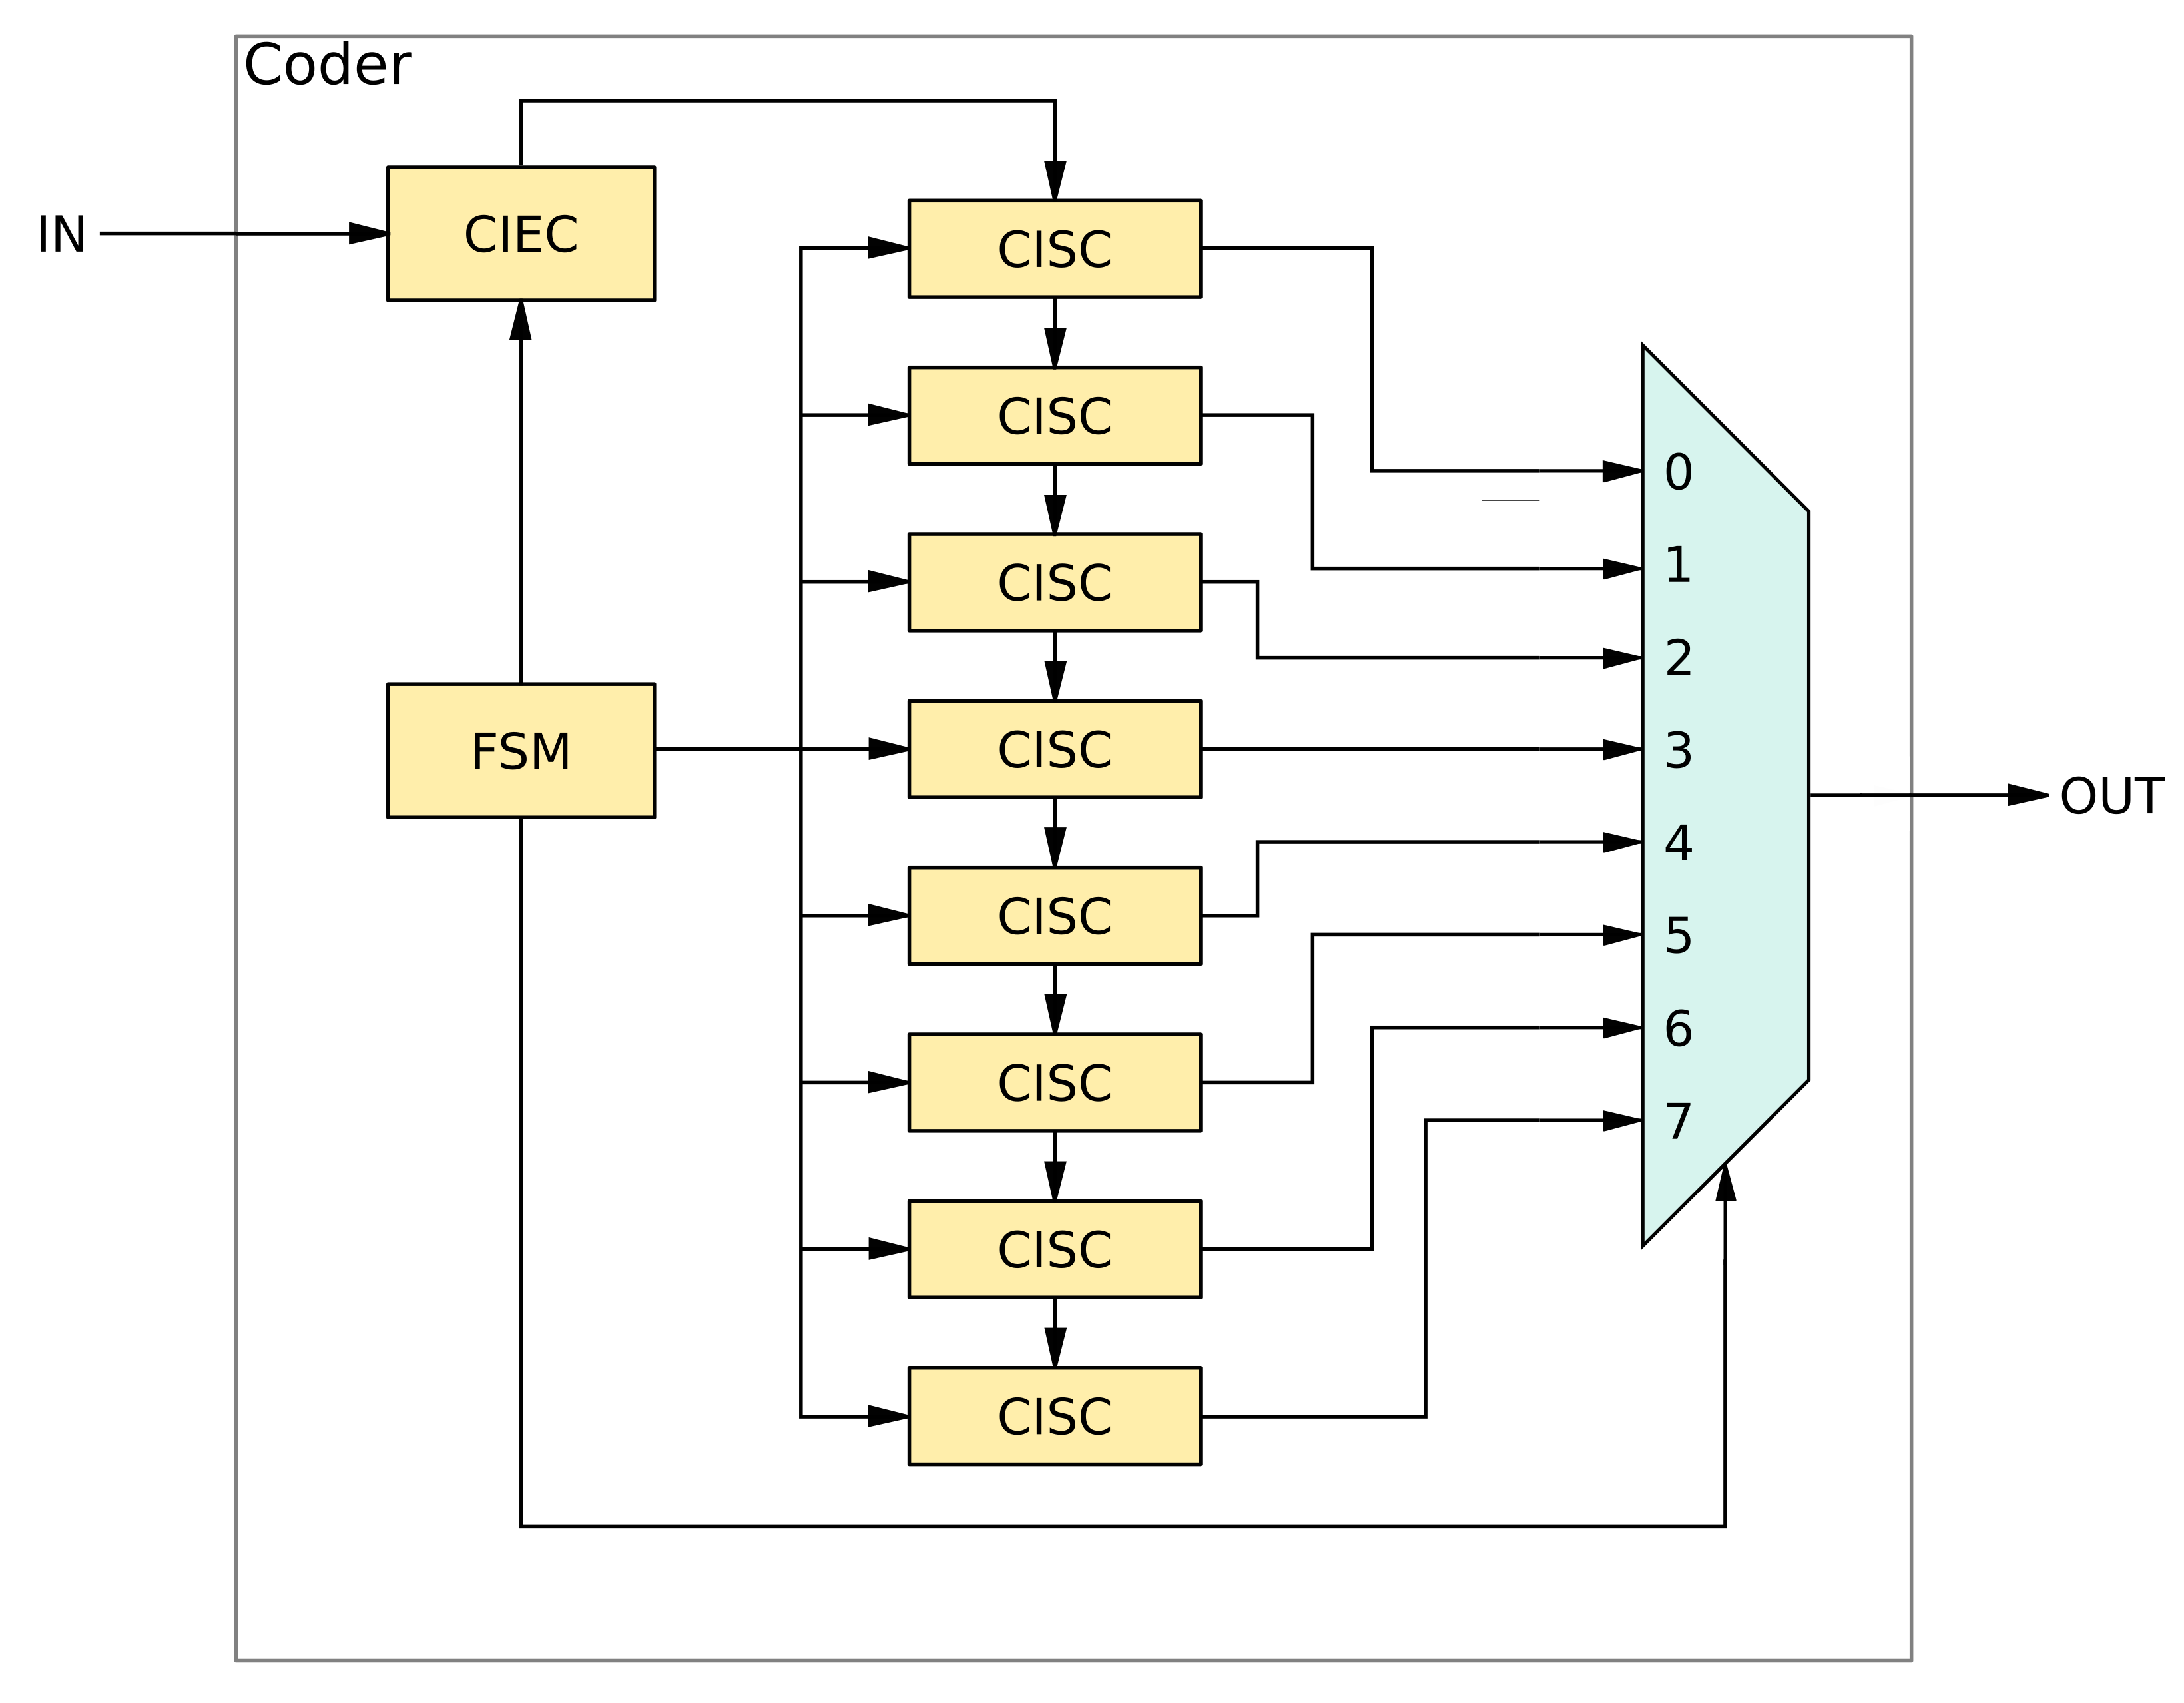
\includegraphics[width=\textwidth]{Diagramas/internal_coder.png}%
        \end{figure}
        \end{column}
        \begin{column}{0.5\linewidth}
        \begin{figure}
            \centering
        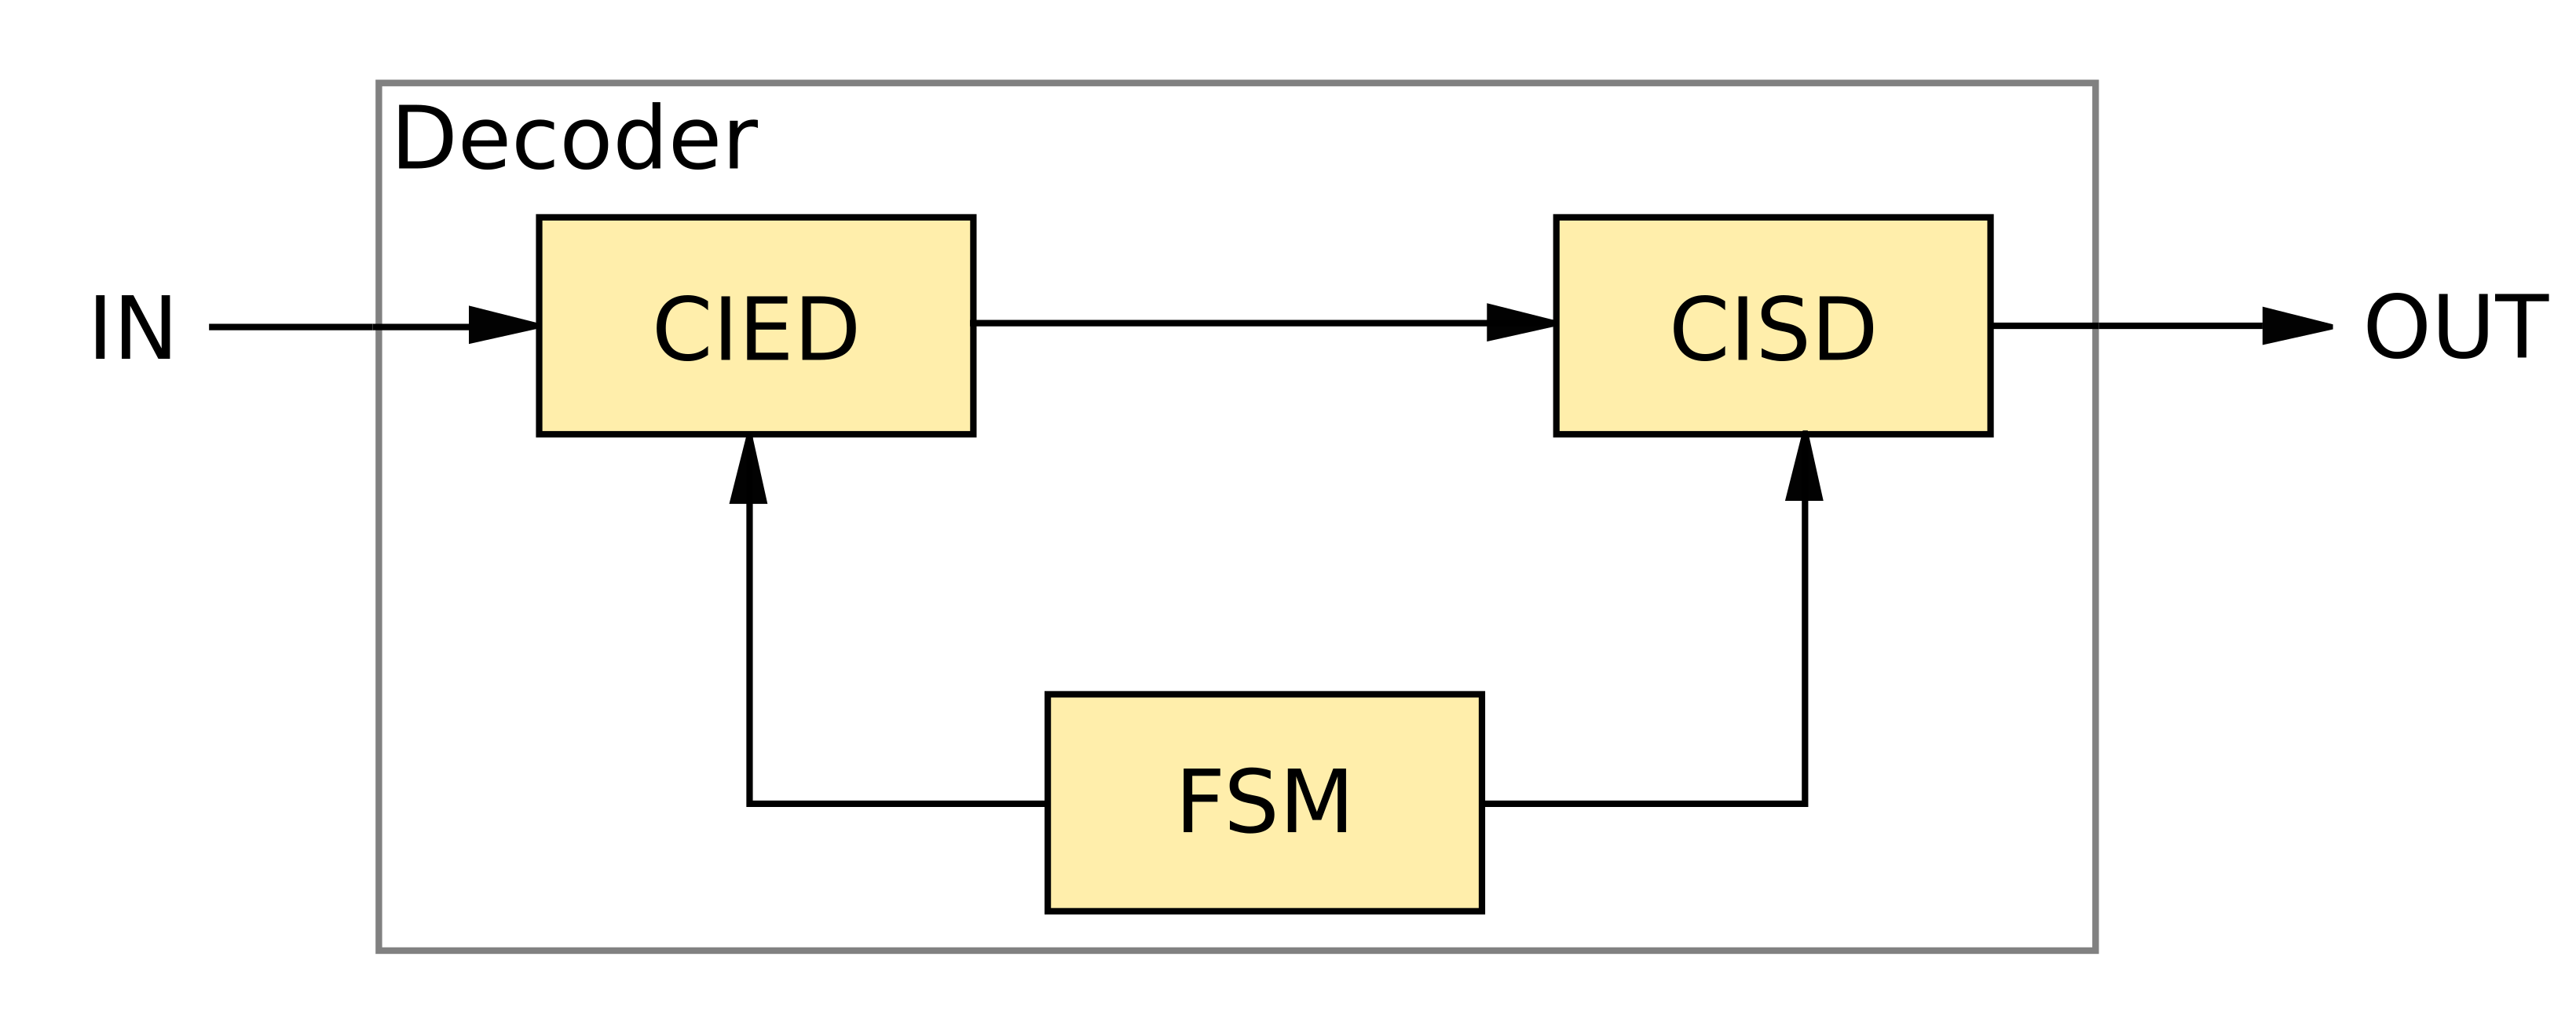
\includegraphics[width=\textwidth]{Diagramas/internal_decoder.png}
        \end{figure}
        \end{column}
    \end{columns}
\end{frame}

\begin{frame}
  \frametitle{\textbf{\textbf{Estructura interna del CIEC}}}
      \framesubtitle{\secname : \subsecname}
        \begin{figure}
                \centering
            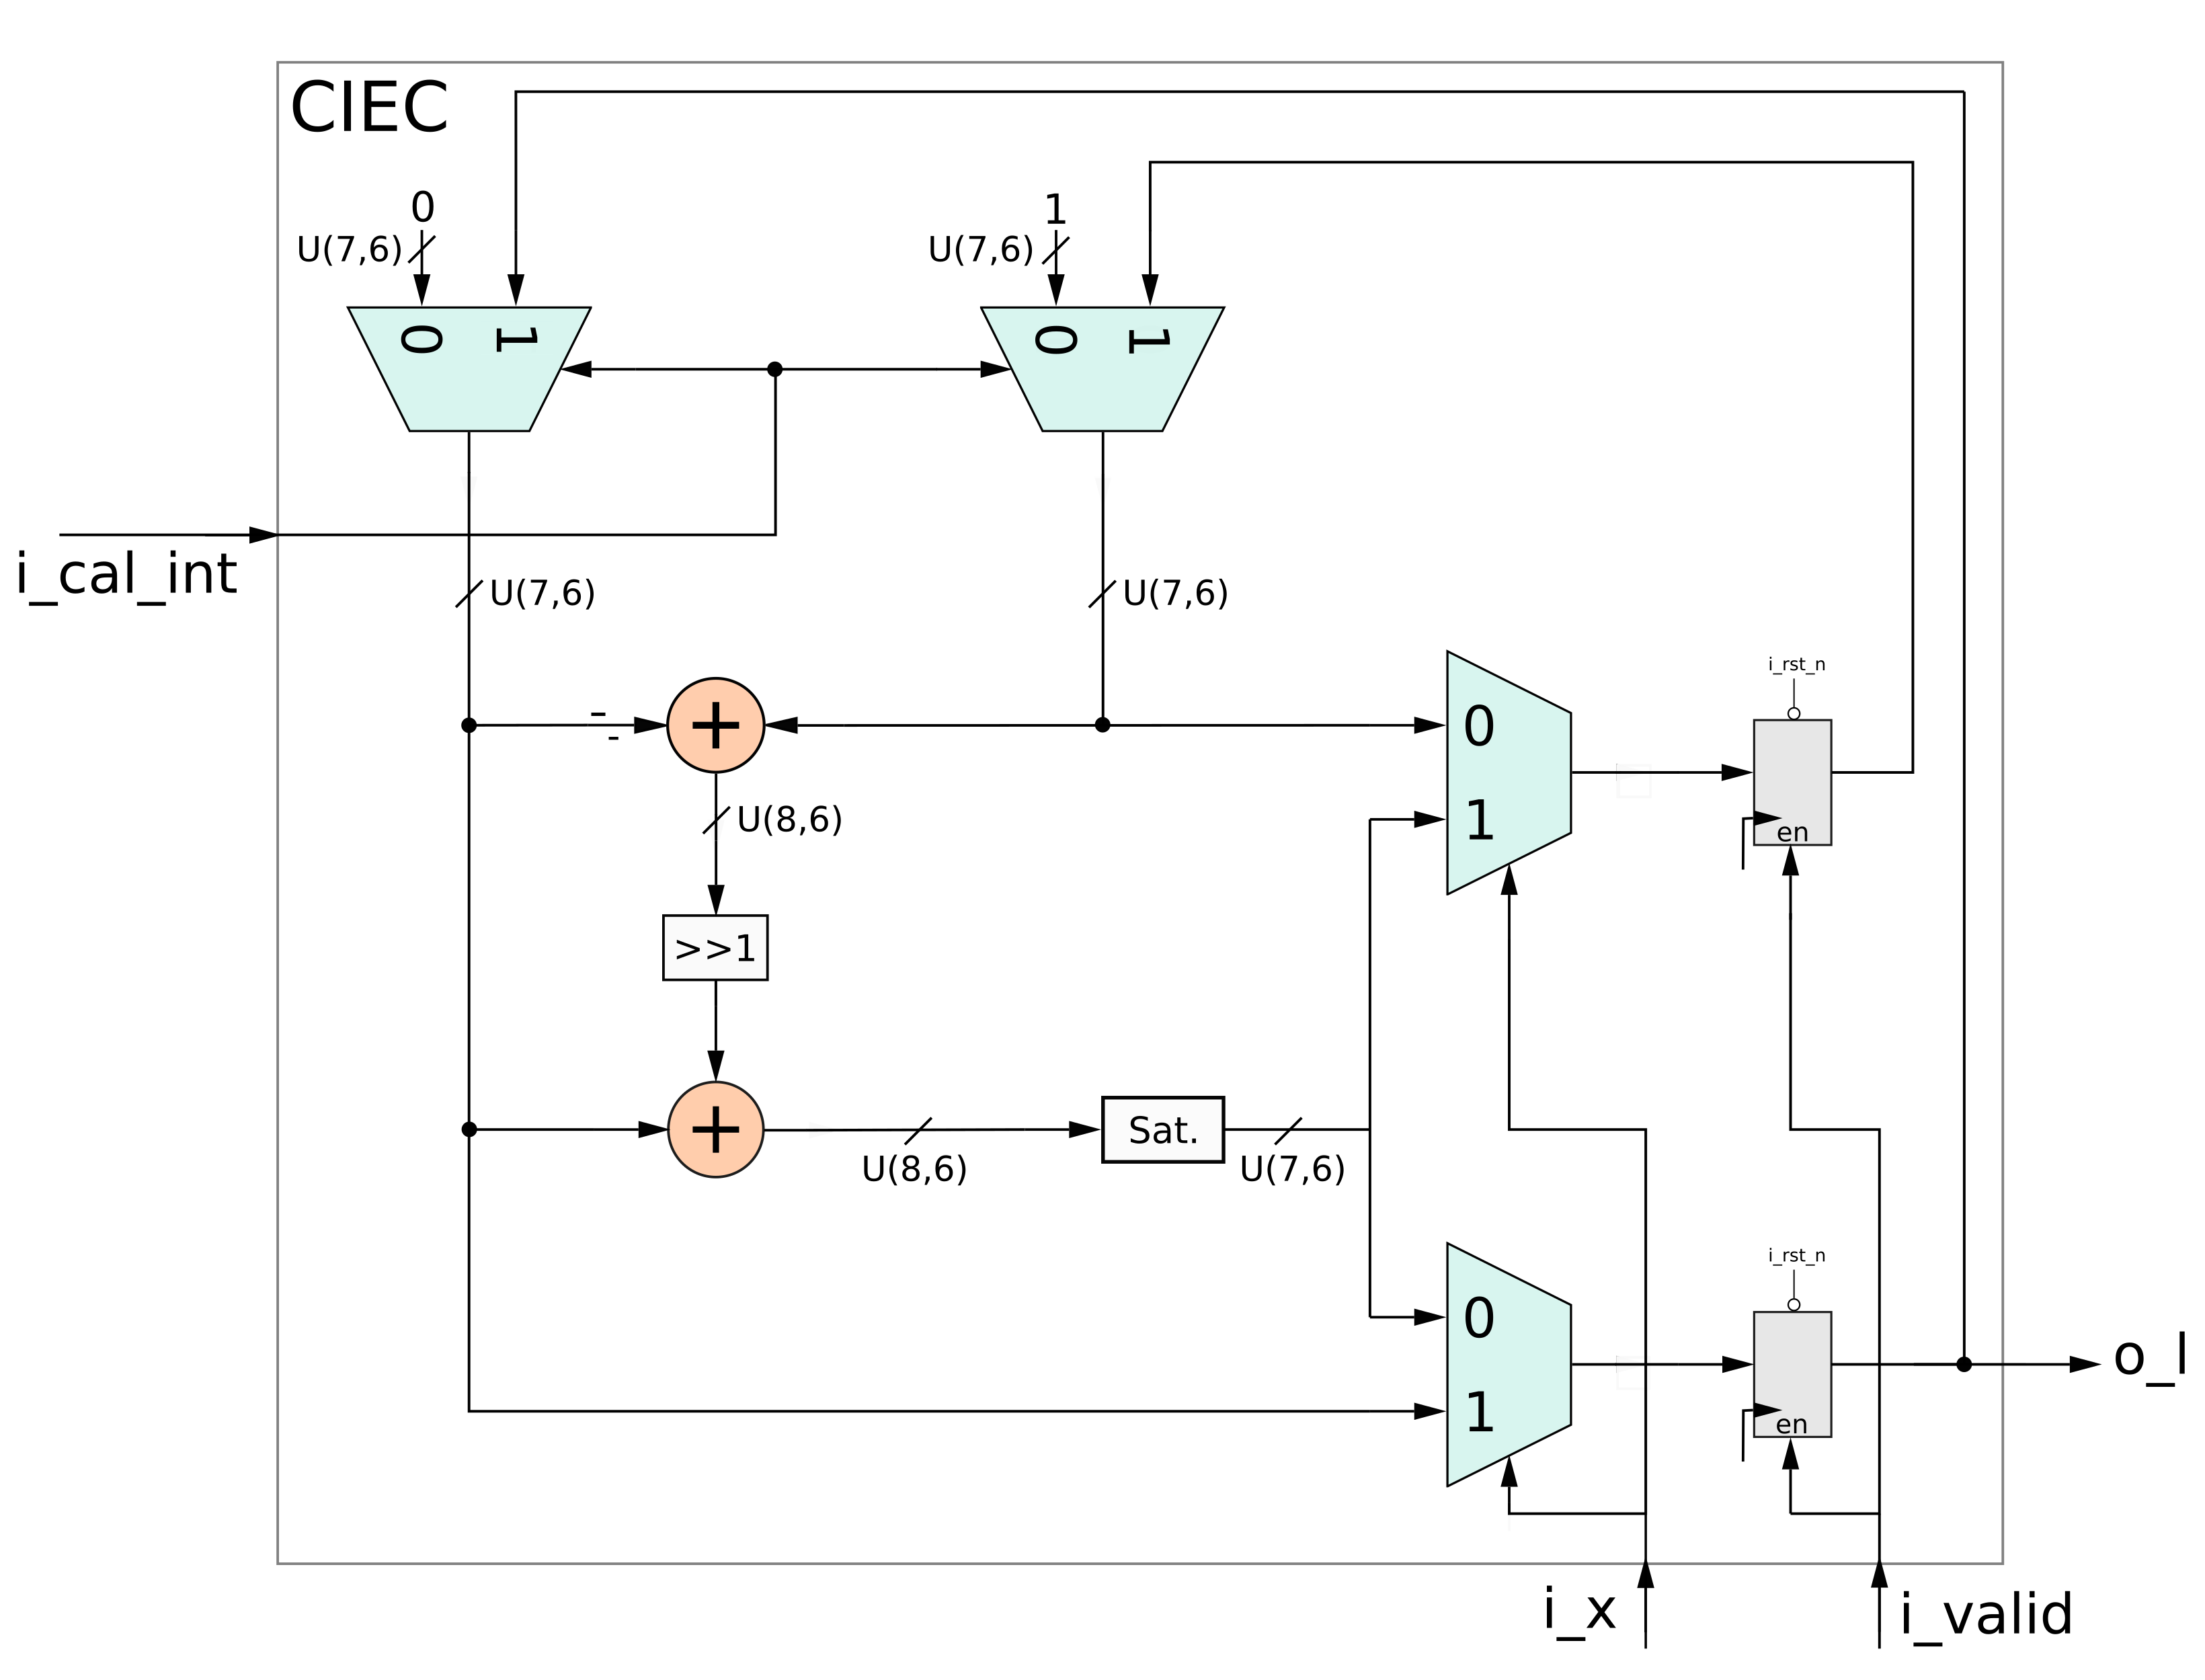
\includegraphics[width=0.8\linewidth]{Diagramas/internal_ciec.png}%
            \end{figure}
\end{frame}

\begin{frame}
  \frametitle{\textbf{\textbf{Estructura interna del CISC}}}
      \framesubtitle{\secname : \subsecname}
        \begin{figure}
                \centering
            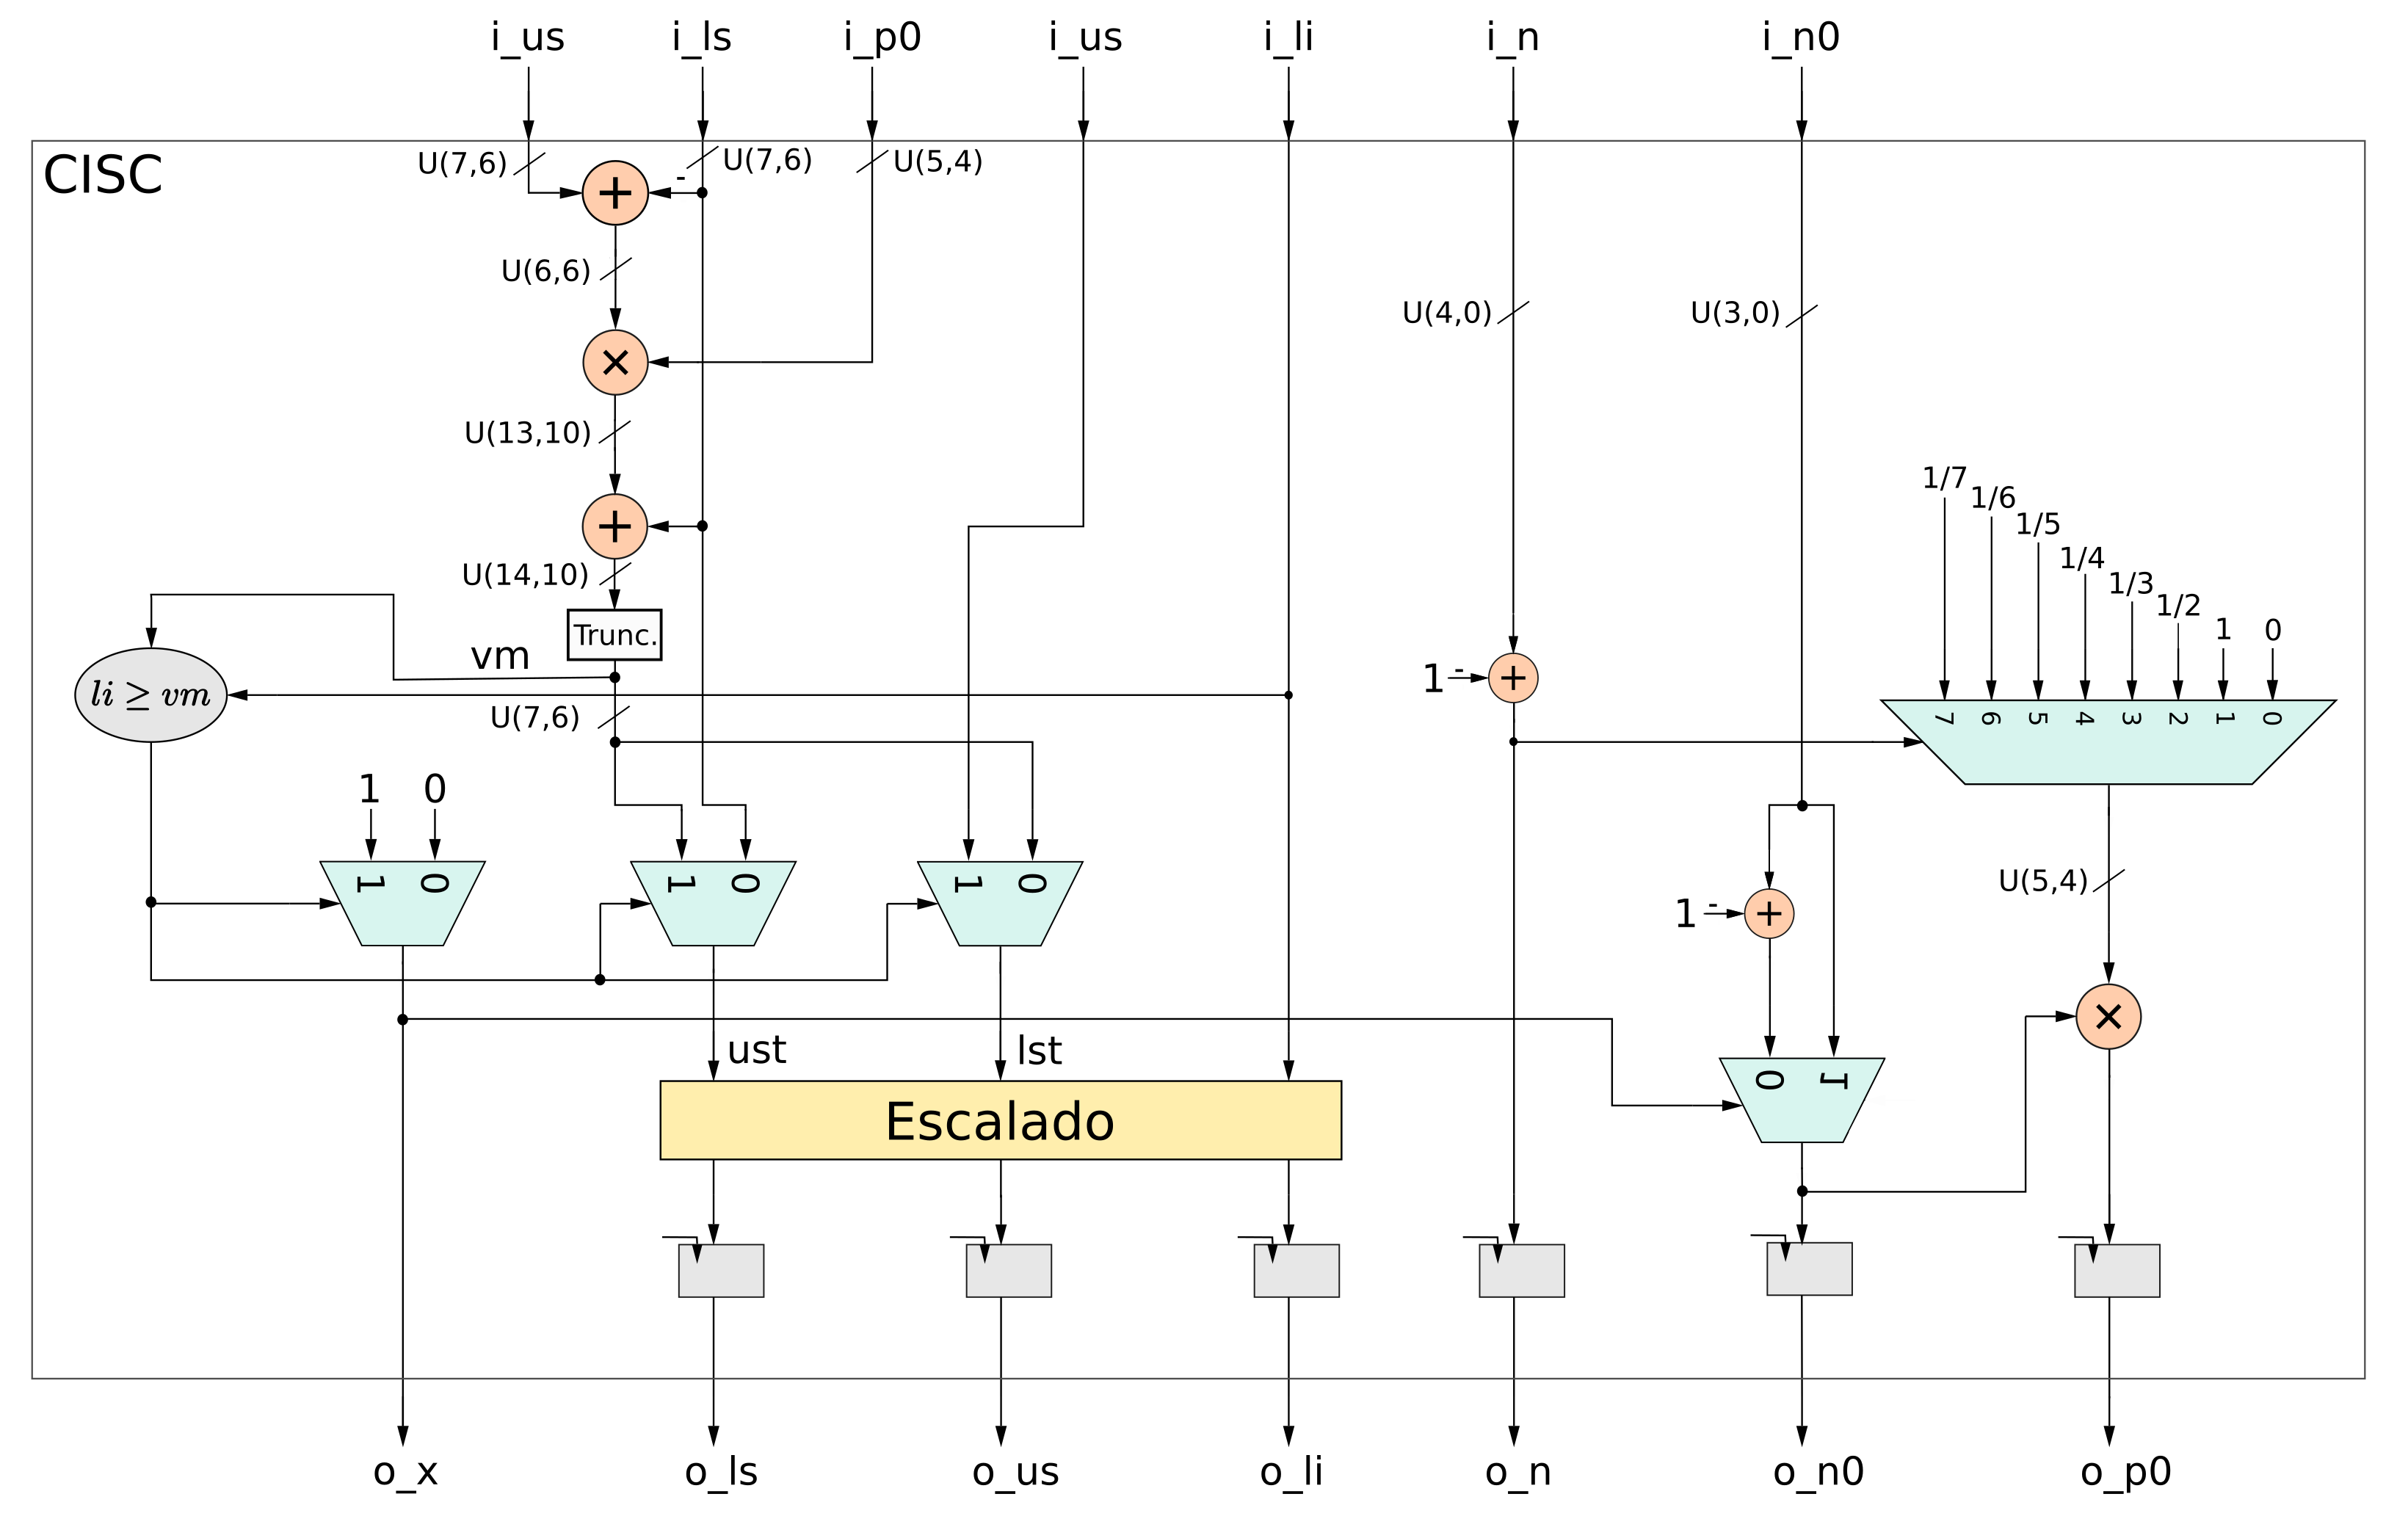
\includegraphics[width=0.8\linewidth]{Diagramas/internal_cisc.png}%
            \end{figure}
\end{frame}


\begin{frame}
  \frametitle{\textbf{\textbf{Bloque codificador y decodificador}}}
          \framesubtitle{\secname : \subsecname}
    \begin{block}{\centering \textbf{Flujo de datos}}
     \begin{itemize}
        \item Los bloques CIEC requiere de 4 u.t. pero es habilitado la mitad de los ciclos, por lo que requieren 8 u.t.
        \item El bloque CISC se ejecuta cada ciclo, por lo que se requieren 8 u.t.
        \item Esto implica que se generan 8 bits de salida cada 16 unidades de tiempo.
    \end{itemize}
    \end{block}
    \vspace{-0.3cm}
  \begin{figure}[!t] \centering
  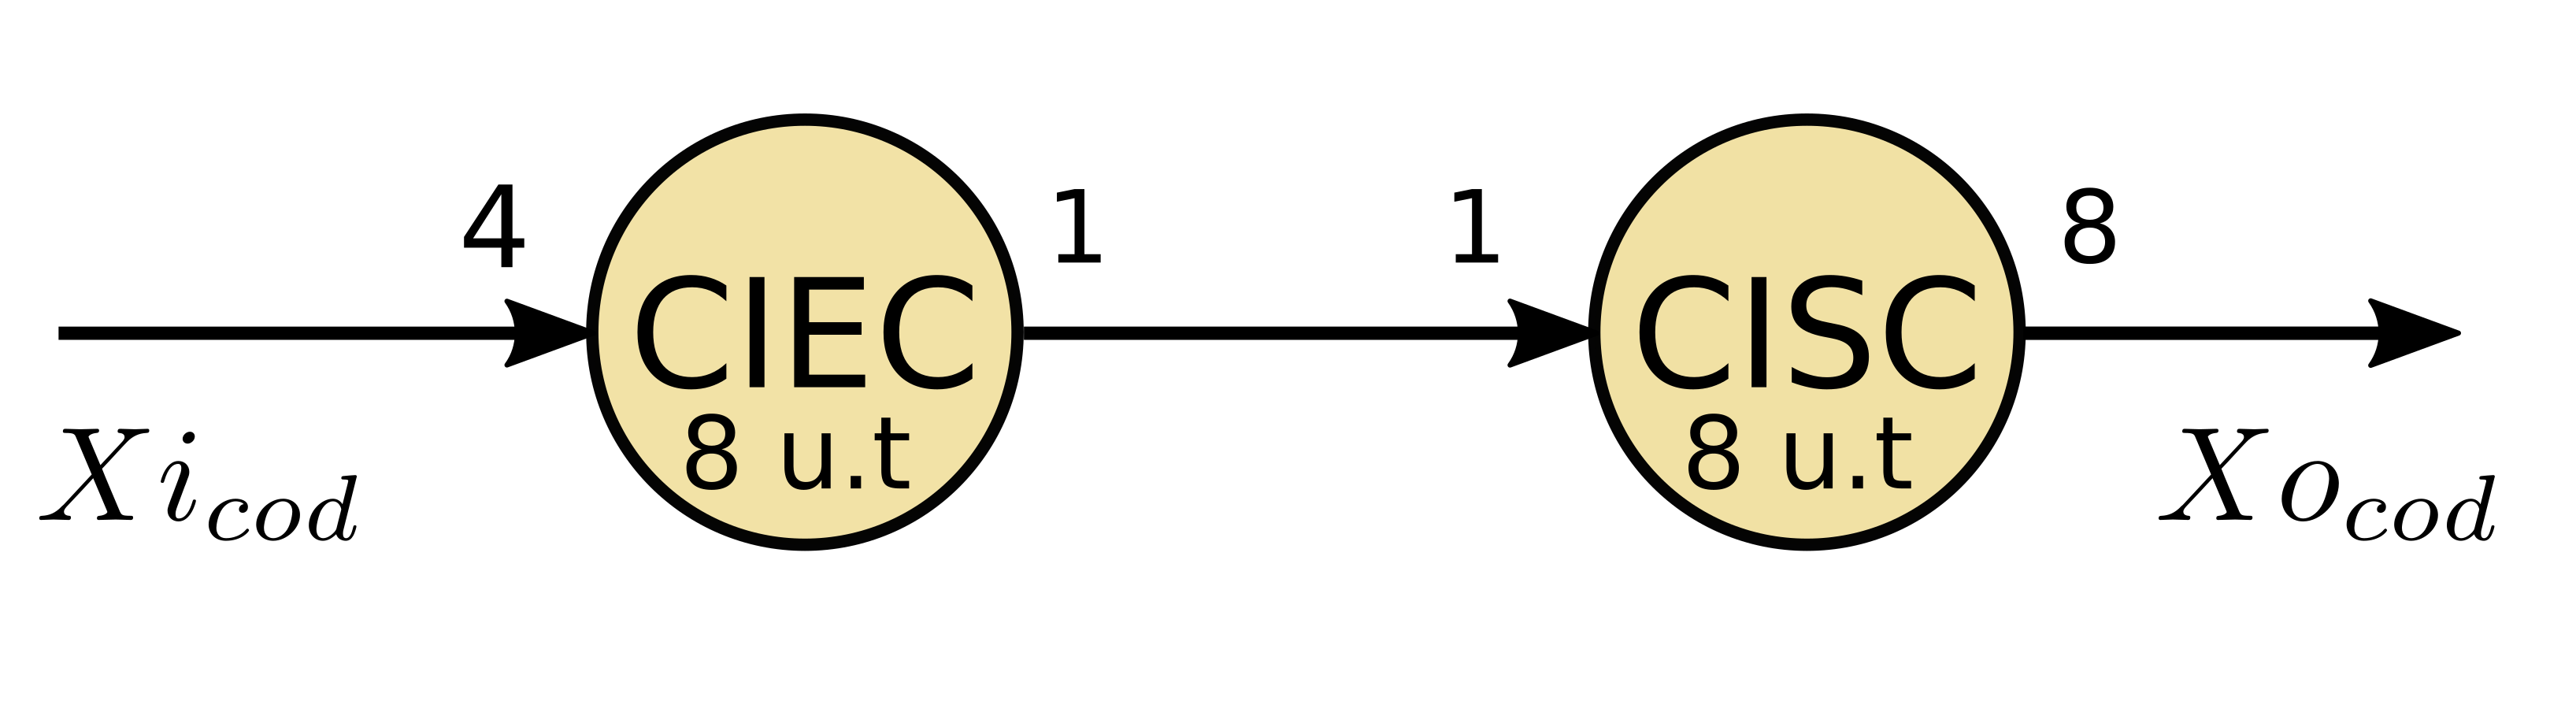
\includegraphics[width=0.70\paperwidth]{Diagramas/grafo_cod.png}%
  \end{figure}
\end{frame}


\begin{frame}
  \frametitle{\textbf{\textbf{Bloque codificador y decodificador}}}
         \framesubtitle{\secname : \subsecname}
    \begin{block}{\centerin \textbf{Ejecución en paralelo}}
        \begin{itemize}
        \item Para evitar un tiempo de procesamiento total de 16 u.t. se corren ambos procesos en paralelo.
        \item Esto implica que se generan 8 bits de salida cada 8 u.t.
    \end{itemize}
    \end{block}
    \vspace{-0.3cm}
  \begin{figure}[!t] \centering
  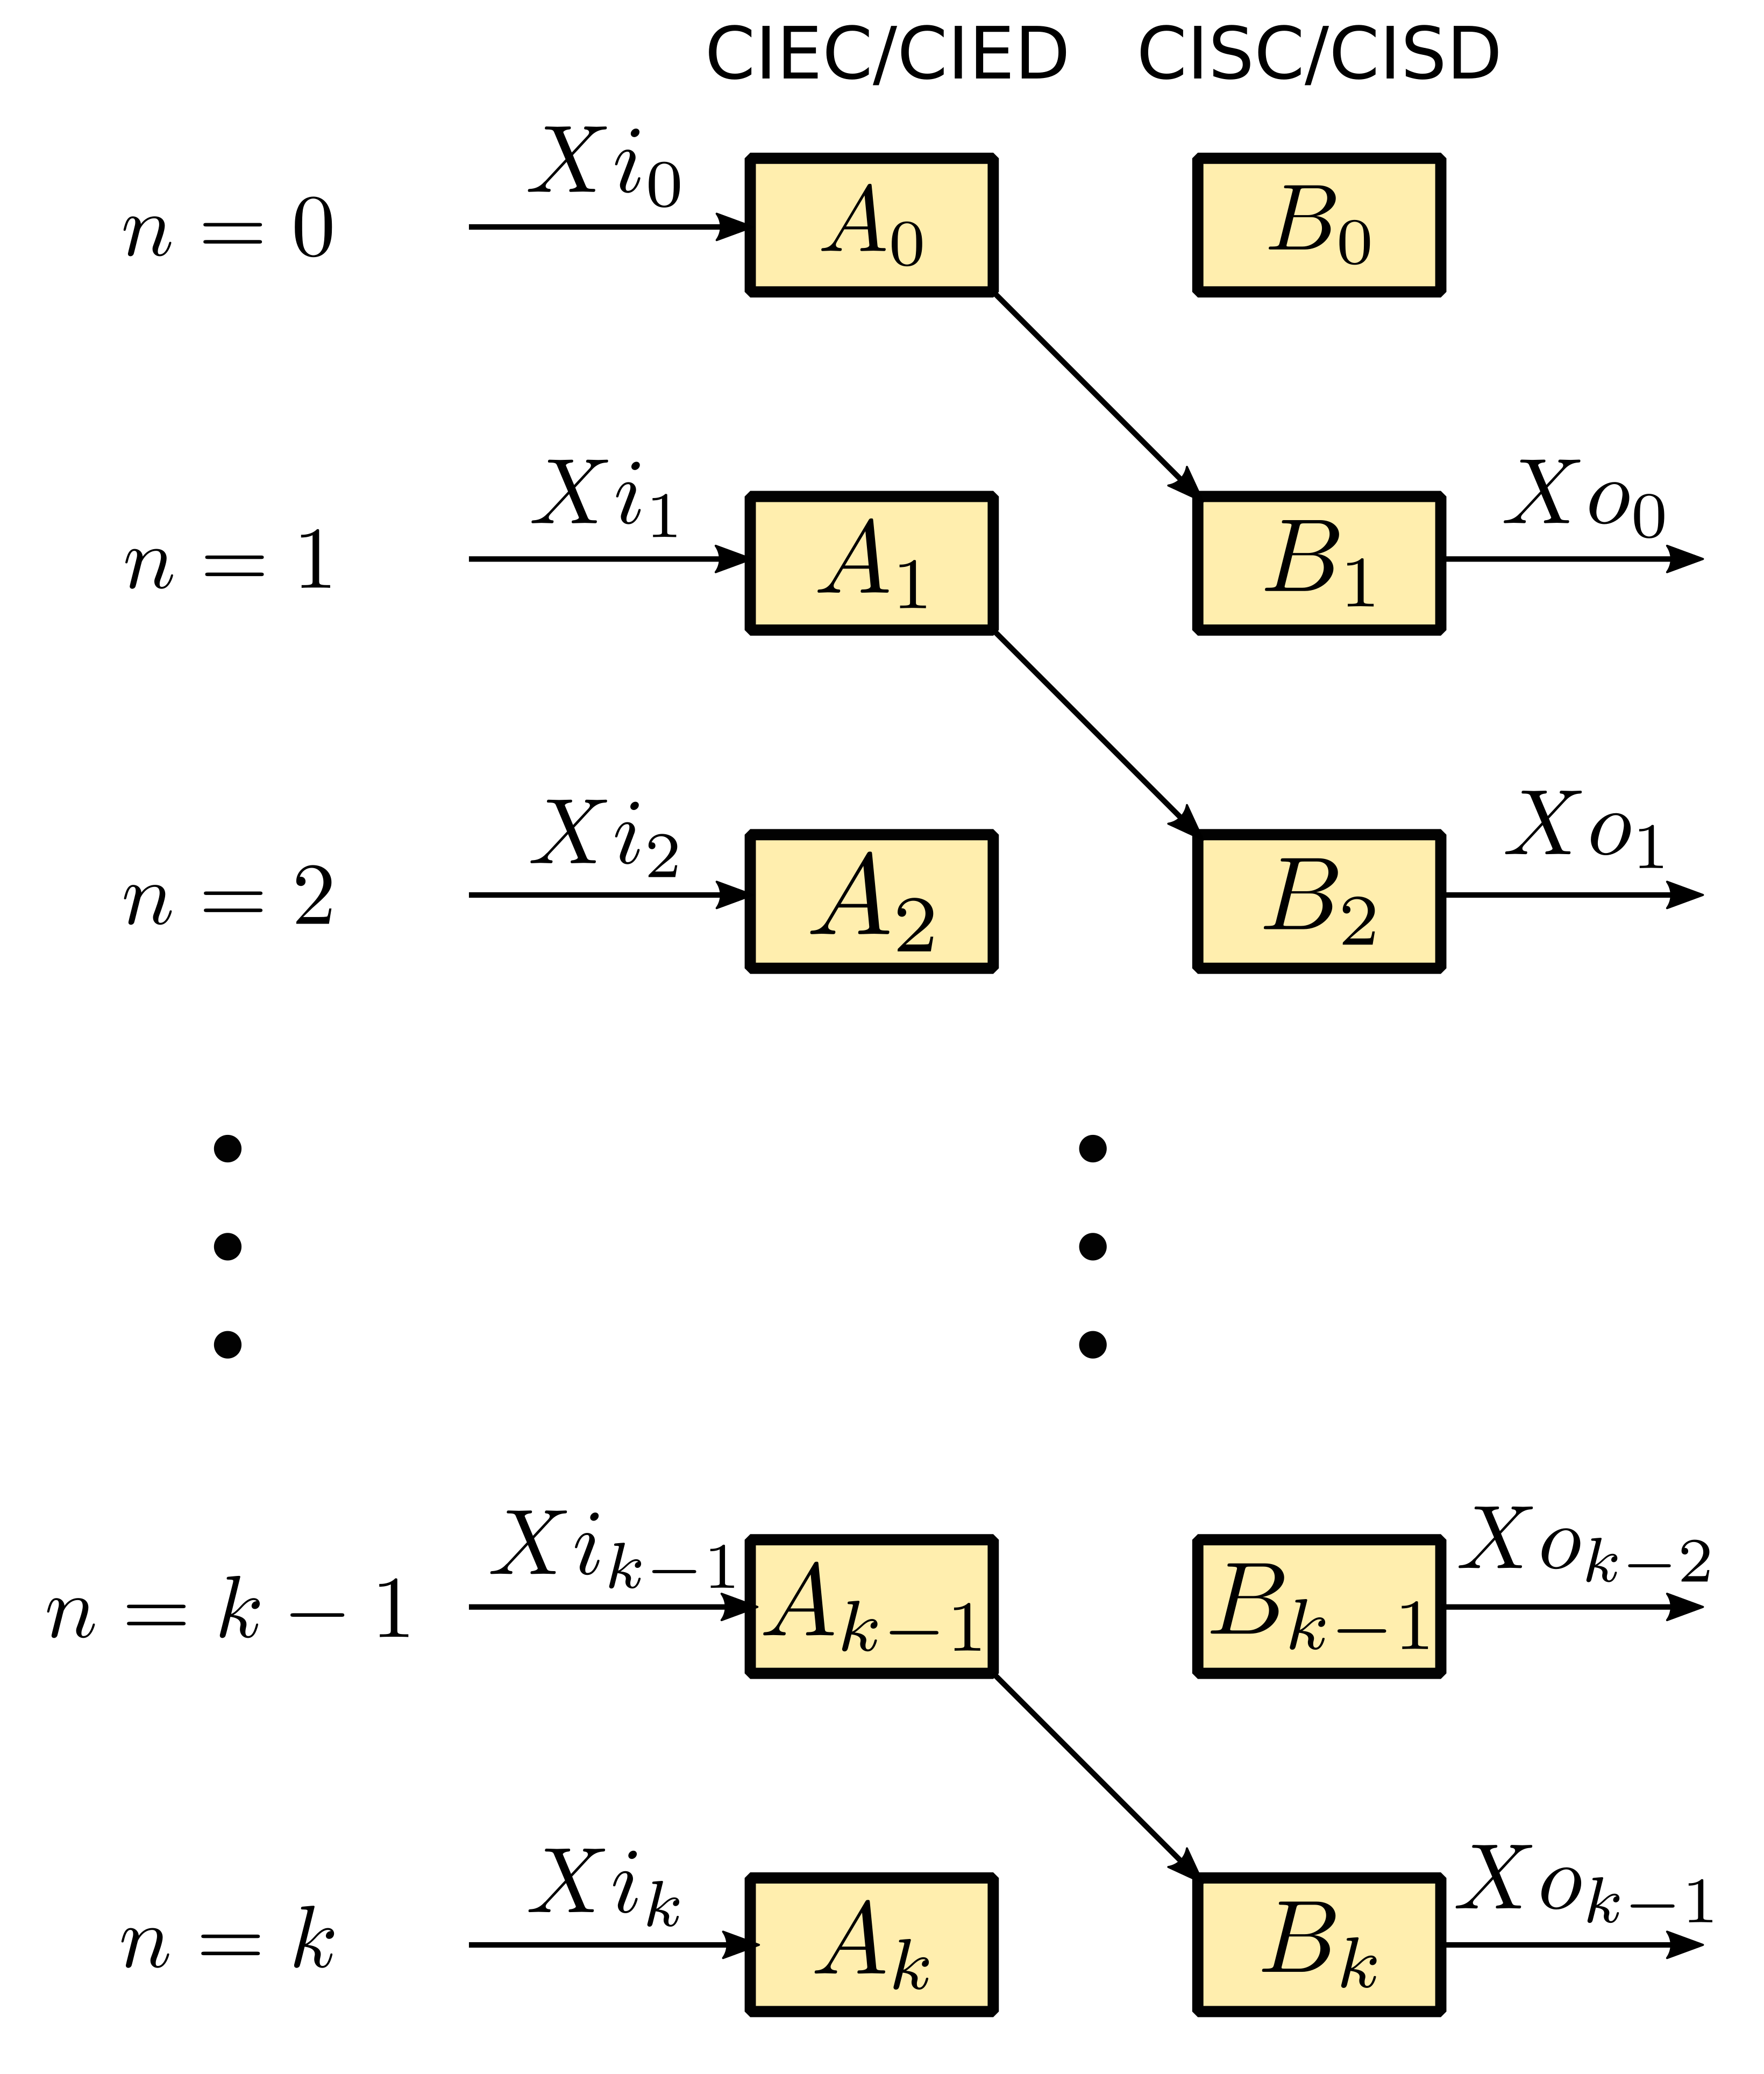
\includegraphics[ height=0.50\paperheight]{Diagramas/dep_graph.png}%
  \end{figure}
\end{frame}



  % Implementación 
%%%%%%%%%%%%%%%%%%%%%%%%%%%%%%%%%%%%%%%%%%%%%%%%%%%%%%%%%%%%%%%%%%% 
%% Desarrollo -  Verificación
%%%%%%%%%%%%%%%%%%%%%%%%%%%%%%%%%%%%%%%%%%%%%%%%%%%%%%%%%%%%%%%%%%%

\subsection{Verificación}
\begin{frame}
  \frametitle{\textbf{Tabla de Contenidos}}
  \begin{center}
    {\vspace{-1.5cm}\Large \textbf{Sección \thesection: \secname }\vspace{0.5cm}}
    \begin{beamercolorbox}[
      sep=8pt,center]{part title}
      \usebeamerfont{part title}
      \textbf{\subsecname}
    \end{beamercolorbox}
  \end{center}
\end{frame}


\begin{frame}
  \frametitle{\textbf{\textbf{Plataforma de verificación}}}
     \framesubtitle{\secname : \subsecname}
    \vspace{-0.3cm}
  \begin{figure}[!t] \centering
  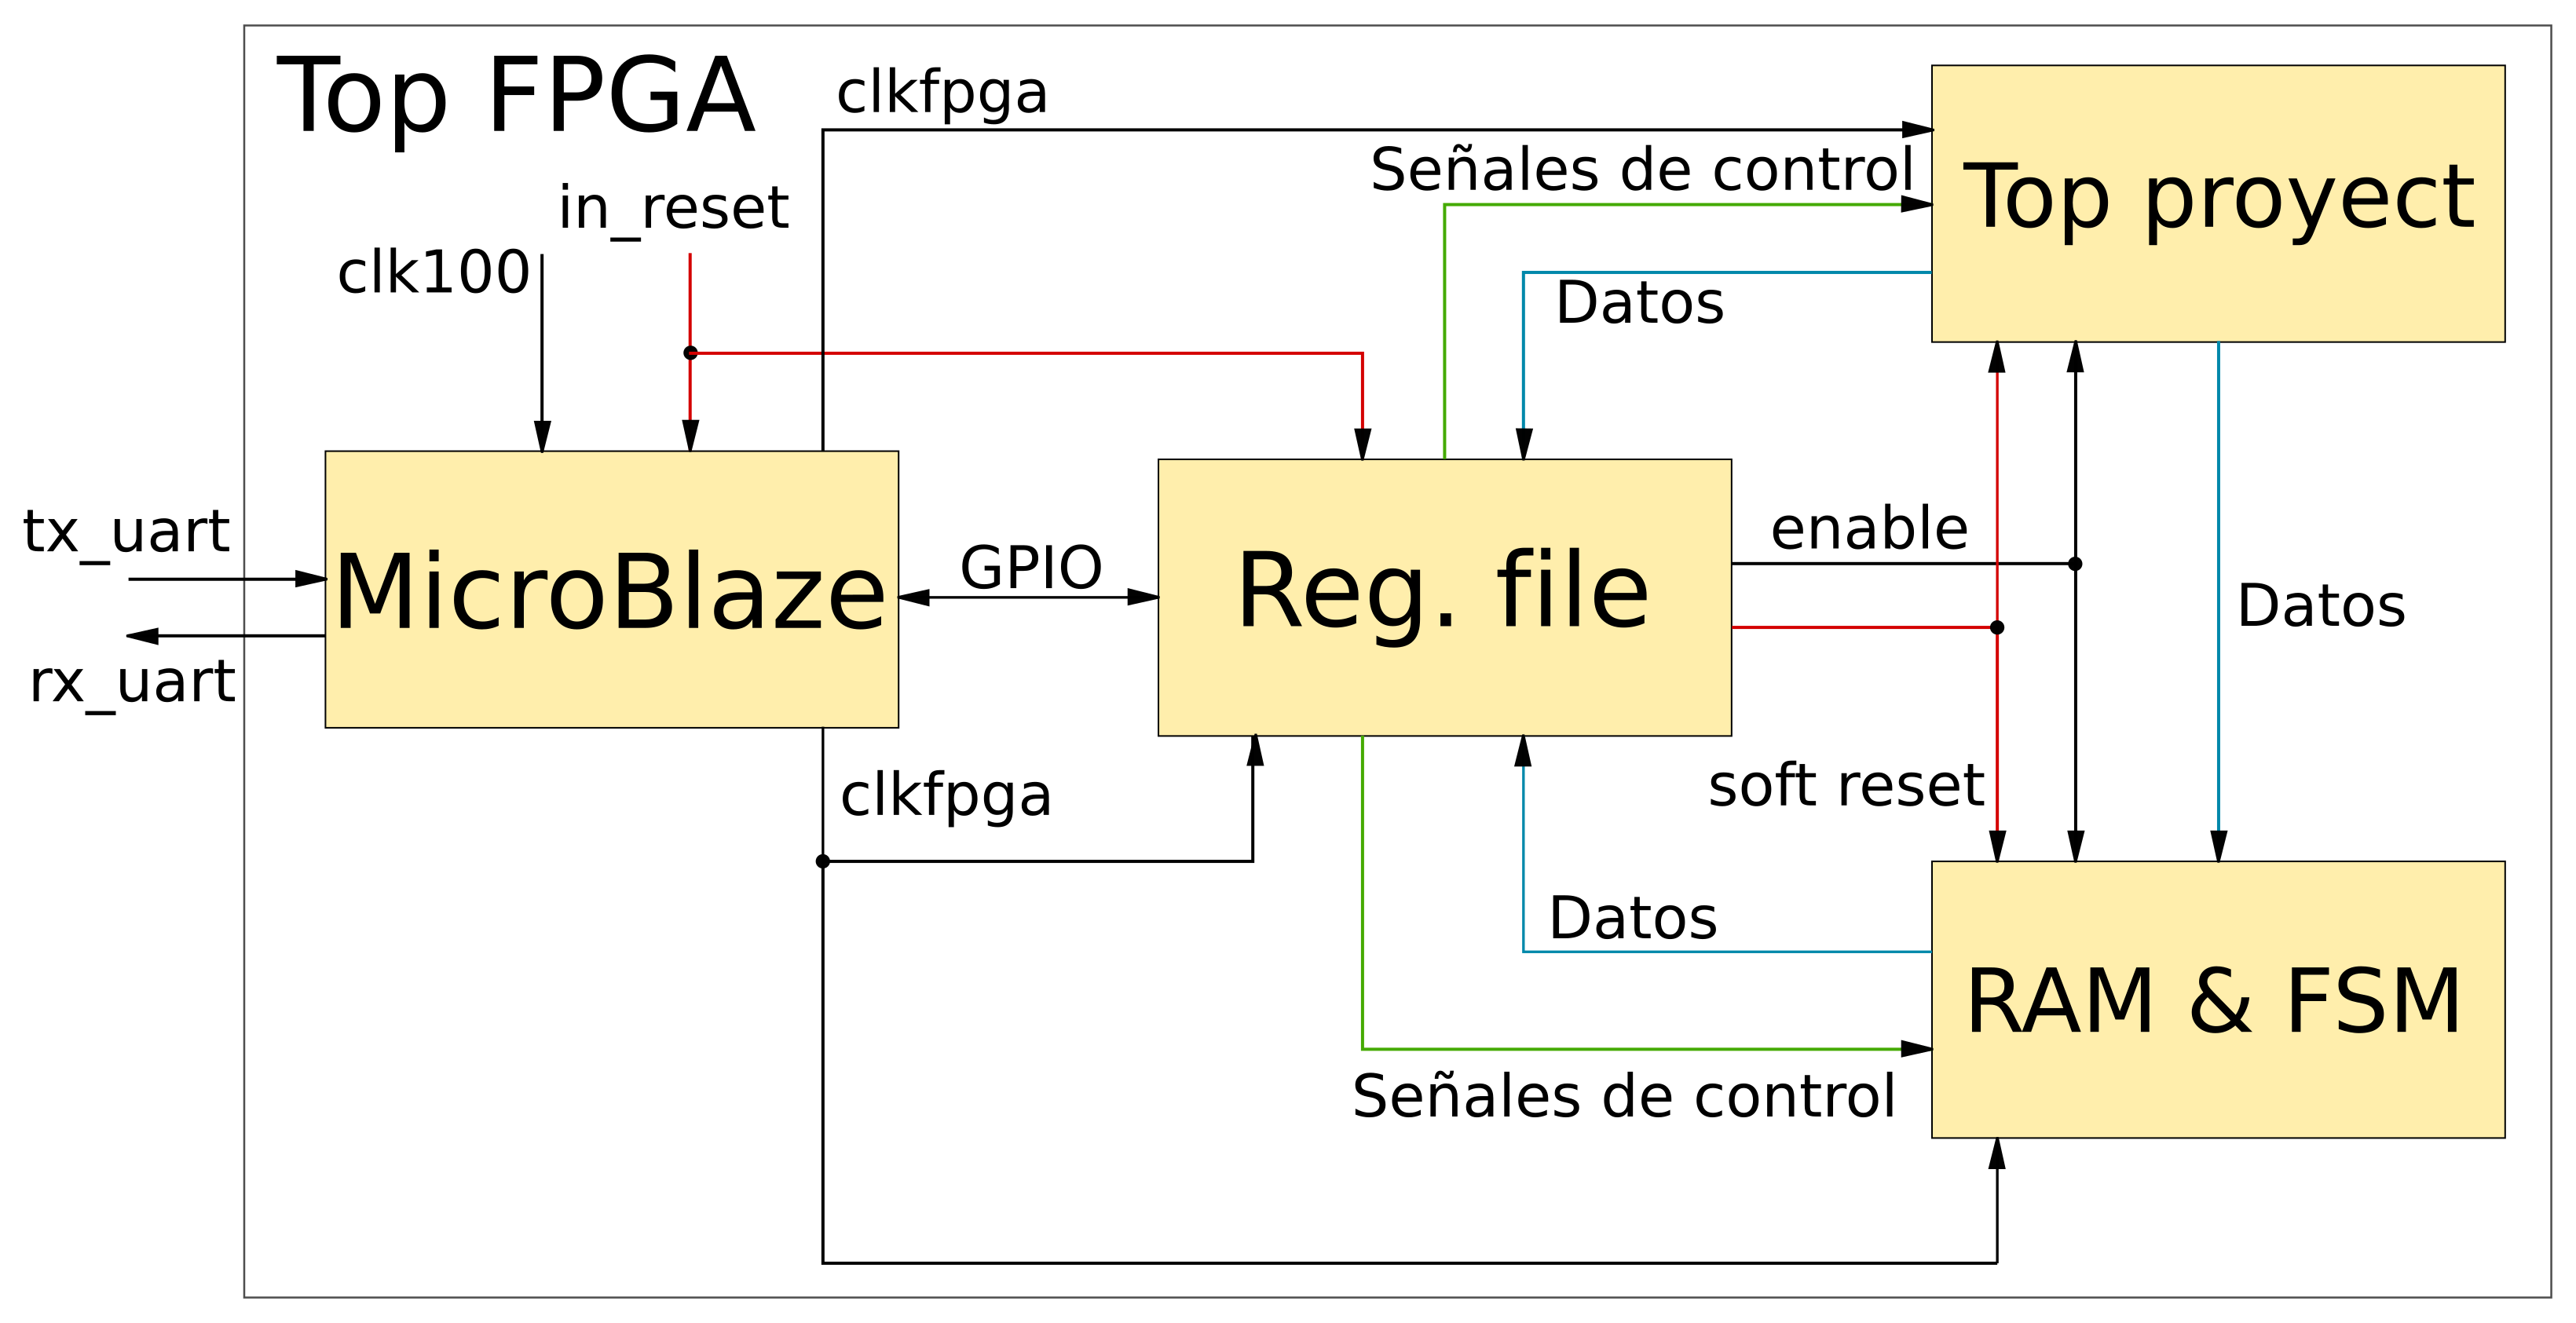
\includegraphics[ width=0.85\paperwidth]{Diagramas/internal_fpga.png}%
  \end{figure}
\end{frame}


% \begin{frame}
%   \frametitle{\textbf{\textbf{Bloques perifericos}}}
%      \framesubtitle{\secname : \subsecname}

%     \begin{block}{\centering \textbf{Generador de bits pseudoaletorios (PRBS)} }
%     \begin{itemize}\small
%         \item Para generar una modulación PAM-4 se utilizan dos PRBS. Una genera el bit de signo mientras y la otra el de magnitud. 
%     \end{itemize}
%     \end{block}
%     \begin{block}{\centering \textbf{Modulo BER}}
%         Consta de dos etapas:
%         \begin{enumerate}\small
%             \item Sincroniza la secuencia de datos decodificada con la secuencia proveniente de la PRBS
%             \item  Dos contadores de 64 bits almacenan la cantidad de muestras de entrada y de errores
%         \end{enumerate}
%     \end{block}
%     \begin{block}{\centering \textbf{Generador de ruido gaussiano (GNG)}}
%         \begin{itemize}\small
%     \item Permite medir niveles de BER extremadamente bajos (~$10^{-15}$). \item El mismo fue obtenido de \cite{gng}. 
%     \end{itemize}
%     \end{block}
% \end{frame}


\begin{frame}
  \frametitle{\textbf{Resultados obtenidos}}
   \framesubtitle{\secname : \subsecname}
   Símbolos codificados, $P_{(x=0)}=0.75$
    \vspace{-0.3cm}

\begin{columns}
    \begin{column}{0.48\linewidth}  
    \begin{figure}
        \centering
    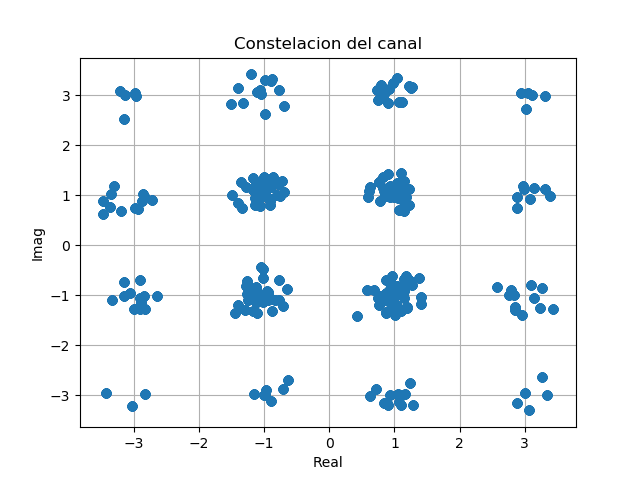
\includegraphics[width=\textwidth]{Graficos/Channel_Constelation.png}%
    \end{figure}
    \end{column}

    \begin{column}{0.48\linewidth}
    \begin{figure}
        \centering
    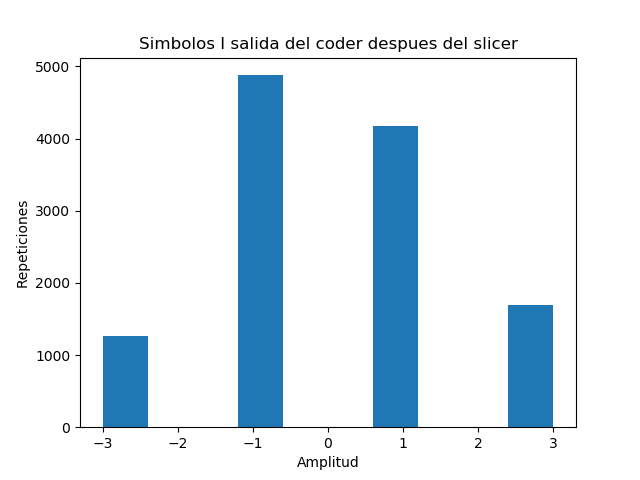
\includegraphics[width=\textwidth]{Graficos/I_symbols_slicer.png}
    \end{figure}
    \end{column}
\end{columns}
\end{frame}

\begin{frame}
  \frametitle{\textbf{Resultados obtenidos}}
   \framesubtitle{\secname : \subsecname}
   Símbolos codificados, $P_{(x=0)}=0.25$
    \vspace{-0.3cm}

\begin{columns}
    \begin{column}{0.48\linewidth}  
    \begin{figure}
        \centering
    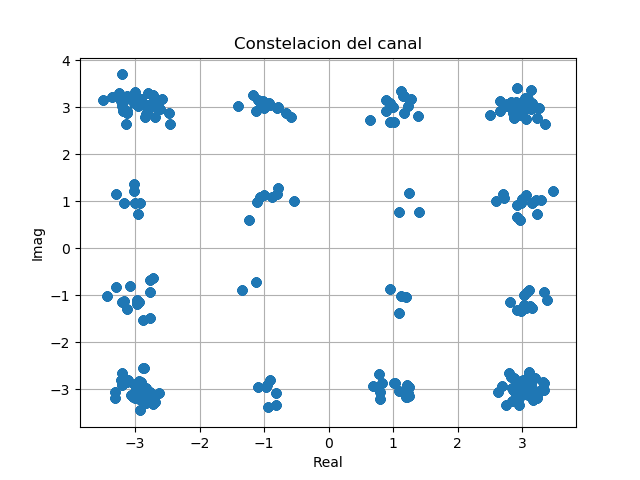
\includegraphics[width=\textwidth]{Graficos/Channel_Constelation_3.png}%
    \end{figure}
    \end{column}

    \begin{column}{0.48\linewidth}
    \begin{figure}
        \centering
    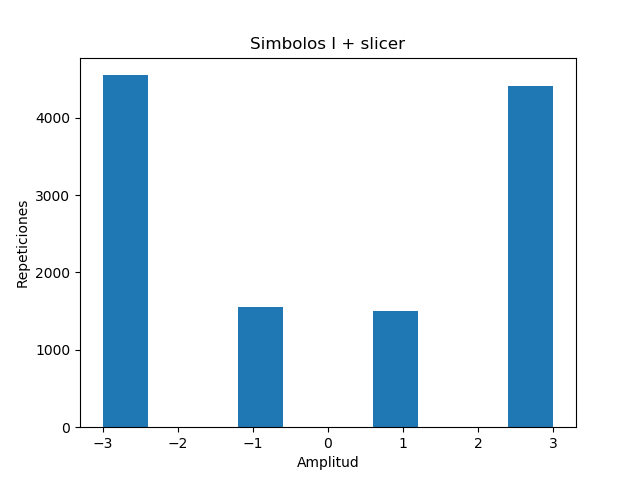
\includegraphics[width=\textwidth]{Graficos/I_symbols_slicer_3.png}
    \end{figure}
    \end{column}
\end{columns}
\end{frame}

  % Verificación
%%%%%%%%%%%%%%%%%%%%%%%%%%%%%%%%%%%%%%%%%%%%%%%%%%%%%%%%%%%%%%%%%%% 
%% Conclusiones 
%%%%%%%%%%%%%%%%%%%%%%%%%%%%%%%%%%%%%%%%%%%%%%%%%%%%%%%%%%%%%%%%%%%



\section{ Conclusiones}
\begin{frame}
  \frametitle{\textbf{Tabla de Contenidos}}
  \begin{center}
    {\vspace{-1.5cm}\Large \textbf{Sección \thesection}\vspace{0.5cm}}
    \begin{beamercolorbox}[
      sep=8pt,center]{part title}
      \usebeamerfont{part title}
      \textbf{\insertsection}
    \end{beamercolorbox}
  \end{center}
\end{frame}


\begin{frame}
  \frametitle{\textbf{\textbf{Conclusiones}}}
    \begin{block}{\centering \textbf{Técnica `probabilistic shaping'}}
    \begin{itemize}\small
        \item Permite disminuir la tasa de error total del sistema.
        \item Agrega una determinada cantidad de bits de redundancia.
        \item Se vuelve mas eficiente a medida que la longitud de entrada aumenta.
    \end{itemize}
    \end{block}
    \vspace{-0.2cm}

    \begin{block}{\centering \textbf{Técnica `constant distribution matching'}}
       \begin{itemize}\small
        \item Se debe utilizar técnica de escalado.
        \item La actualización de la nueva probabilidad implica realizar una división.
        \item Fácil adaptación a nuevas distribuciones de probabilidad. 
    \end{itemize}
    \end{block}
    \vspace{-0.2cm}

    \begin{block}{\centering \textbf{Implementación}}
    \begin{itemize}\small
        \item El calculo de los intervalos, se puede realizar de manera recursiva o secuencial.
        \item  El sistema implementado es poco practico para una longitud de entrada de 4 bits. 
    \end{itemize}
    \end{block}
\end{frame}  % Conclusión





\section{Bibliografía}
\begin{frame}%[t,allowframebreaks]
  \frametitle{Bibliografía}
  % \vspace{-0.7cm}
  \tiny
  %\bibliographystyle{./IEEEtranBST/IEEEtran}
  \bibliographystyle{ieeetr}
  \bibliography{./biblio.bib}
\end{frame}


\begin{frame}
  \frametitle{\textbf{Preguntas}}
   \begin{center}
     {\Huge \textbf{Muchas Gracias!}\\}
    \end{center}
\end{frame}

\end{document}
